\documentclass[a4paper]{article}    % define document layout
%\documentclass[draft]{article}     % use draft option in packages
%-----------------------------
% preamble
%-----------------------------
\usepackage[sumlimits,]{amsmath}    % math equations and formulas
\usepackage[utf8]{inputenc}         % use UTF-8 encoding
\usepackage[english]{babel}         % use English language
\usepackage{graphicx}              % insert images
%\usepackage[draft]{graphicx}        % do not render figures
\usepackage{subcaption}             % multiple images in one figure
\usepackage{hyperref}               % hyperlinks
\usepackage{float}                  % floating objects (figures, tables)
\usepackage{geometry}               % page size and margins
\geometry{a4paper, margin=1in}      % margins
\usepackage{ragged2e}               % text alignment
%\usepackage{multirow}               % merge rows in table

\graphicspath{                      % path for figures
    {../figures/} 
    {../figures/mlp/} 
    {../figures/svm/} 
}

%-----------------------------
% body
%-----------------------------
\begin{document}

\begin{figure}
    \centering
    % UNICAMP logo
    \begin{subfigure}{0.45\textwidth}
        \centering
        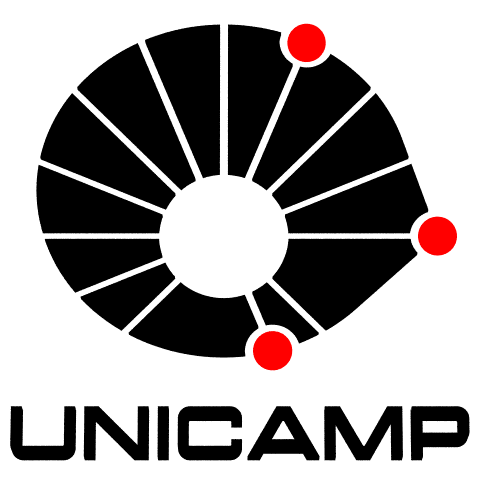
\includegraphics[width=1.5cm]{unicamp}
%        \label{fig:unicamp}
    \end{subfigure}
    \hfill
    % FEEC logo
    \begin{subfigure}{0.45\textwidth}
        \centering
        
\includegraphics[width=1.5cm]{feec}
%        \label{fig:feec}
    \end{subfigure}
\end{figure}

\title{EFC3 - Exercise 3}
\author{Rafael Claro Ito (R.A.: 118430)}
%R.A.: 118430
%ito.rafael@gmail.com
\date{November 2019}
\maketitle
\newpage

%=================================================
\section{Source files}
%=================================================

\paragraph{All code cited and all figures showed here can be found at the following GitHub repository:\\
\url{https://github.com/ito-rafael/IA006C-MachineLearning/tree/master/efc3}\\
In this repository, one can found the following files:\\}

\begin{itemize}
    \item Jupyter Notebook
    \begin{itemize}
        \item \href{https://github.com/ito-rafael/IA006C-MachineLearning/tree/master/efc3/notebooks}{MLP.ipynb}
        \item \href{https://github.com/ito-rafael/IA006C-MachineLearning/blob/master/efc3/notebooks/SVM.ipynb}{SVM.ipynb}
    \end{itemize}
    \item \LaTeX
    \begin{itemize}
        \item \href{https://github.com/ito-rafael/IA006C-MachineLearning/blob/master/efc3/latex/efc3.tex}{efc3.tex}
    \end{itemize}
\end{itemize}

\paragraph{The notebook ``MLP'' implements a multi-layer perceptron network used for binary classification. Here, we use different numbers of neurons, plot the decision regions and also calculate some metrics to evaluate the overall performance.}

\paragraph{The notebook ``SVM'' uses the same dataset and also implements a binary classifier, but it does this using a support vector machine. Here, we plot the decision regions as well, but this time we vary the value of the hyperparameter C and also the value gamma used in a RBF kernel.}

\bigskip

%=================================================
\section{Part I - Error backpropagation}
%=================================================

$ u_1 = 1 \cdot v_{00} + x_1 \cdot v_{10} + x_2 \cdot v_{20} $\\
$ u_2 = 1 \cdot v_{01} + x_1 \cdot v_{11} + x_2 \cdot v_{21} $\\
$ u_3 = 1 \cdot v_{02} + x_1 \cdot v_{12} + x_2 \cdot v_{22} $\\
\vspace{0.1mm}\\
%
$ s_1 = f(u_1) $\\
$ s_2 = f(u_2) $\\
$ s_3 = f(u_3) $\\
\vspace{0.1mm}\\
%
$ y_1 = 1 \cdot w_{00} + s_1 \cdot w_{10} + s_2 \cdot w_{20} + s_3 \cdot w_{30} $\\
$ y_2 = 1 \cdot w_{01} + s_1 \cdot w_{11} + s_2 \cdot w_{21} + s_3 \cdot w_{31} $\\
\vspace{0.1mm}\\
%
$ J = e_1^2 + e_2^2 $\\
\vspace{0.1mm}\\
%
$ \delta_3 = \dfrac{\partial J}{\partial u_3} = \dfrac{\partial [(d_1-y_1)^2+(d_2-y_2)^2]}{\partial u_3} $\\
$ \delta_3 = \dfrac{\partial (d_1-y_1)^2}{\partial u_3} + \dfrac{\partial (d_2-y_2)^2}{\partial u_3} $\\
$ \delta_3 = \dfrac{\partial (d_1-y_1)^2}{\partial (d_1-y_1)} \cdot \dfrac{\partial (d_1-y_1)}{\partial u_3} + \dfrac{\partial (d_2-y_2)^2}{\partial (d_2-y_2)} \cdot \dfrac{\partial (d_2-y_2)}{\partial u_3} $\\
$ \delta_3 = 2(d_1-y_1) \cdot \left(-\dfrac{\partial y_1}{\partial u_3}\right) + 2(d_2-y_2) \cdot \left(-\dfrac{\partial y_2}{\partial u_3}\right) $\\
$ \delta_3 = - 2(d_1-y_1) \cdot \dfrac{\partial y_1}{\partial s_3} \cdot \dfrac{\partial s_3}{\partial u_3} - 2(d_2-y_2) \cdot \dfrac{\partial y_2}{\partial s_3} \cdot \dfrac{\partial s_3}{\partial u_3} $
%$ \delta_3 = - 2(d_1-y_1) \cdot \dfrac{\partial (1 \cdot w_{00} + s_1 \cdot w_{10} + s_2 \cdot w_{20} + s_3 \cdot w_{30})}{\partial s_3} \cdot \dfrac{\partial f(u_3)}{\partial u_3} - 2(d_2-y_2) \cdot \dfrac{\partial (1 \cdot w_{01} + s_1 \cdot w_{11} + s_2 \cdot w_{21} + s_3 \cdot w_{31})}{\partial s_3} \cdot \dfrac{\partial f(u_3)}{\partial u_3} $\\
\begin{multline*}
    \delta_3 = - 2(d_1-y_1) \cdot \dfrac{\partial (1 \cdot w_{00} + s_1 \cdot w_{10} + s_2 \cdot w_{20} + s_3 \cdot w_{30})}{\partial s_3} \cdot \dfrac{\partial f(u_3)}{\partial u_3} \\
    - 2(d_2-y_2) \cdot \dfrac{\partial (1 \cdot w_{01} + s_1 \cdot w_{11} + s_2 \cdot w_{21} + s_3 \cdot w_{31})}{\partial s_3} \cdot \dfrac{\partial f(u_3)}{\partial u_3}
\end{multline*}
%
$ \delta_3 = - 2(d_1-y_1)\dot{f}(u_3)w_{30} - 2(d_2-y_2)\dot{f}(u_3)w_{31} $\\
\vspace{0.1mm}\\
%
$ \dfrac{\partial J}{\partial v_{12}} = \dfrac{\partial J}{\partial u_3} \cdot \dfrac{\partial u_3}{\partial v_{12}} $\\
$ \dfrac{\partial J}{\partial v_{12}} = \dfrac{\delta_3 \cdot \partial(1 \cdot v_{02} + x_1 \cdot v_{12} + x_2 \cdot v_{22})}{\partial v_{12}} $\\
$ \dfrac{\partial J}{\partial v_{12}} = \delta_3 \cdot x_1 $\\
$ \boxed{ \dfrac{\partial J}{\partial v_{12}} = -2x_1\dot{f}(u_3)[w_{30}(d_1-y_1) + w_{31}(d_2-y_2)] }$\\
\vspace{0.1mm}

%=================================================
\section{Part II - Binary Classification with MLP and SVMs}
%=================================================

%=================================================
\subsection{Multi-layer Perceptron (MLP)}
%=================================================

%--------------------------------------
\subsubsection{a) MLP network}
%--------------------------------------

\paragraph{The MLP network was implemented with the scikit-learn ``MLPClassifier'' class. This model optimizes the log-loss function. The parameters of the network were constantly modified in order to tune the classifier. The final configuration was:}

\paragraph{Parameters:}
\begin{itemize}
    \item number of neurons: 50
    \item activation: relu
    \item solver: adam
    \item alpha: 0.01
    \item batch\_size: 200
    \item random\_state: 42
    \item tol: 1e-3
    \item max\_iter: 1
    \item warm\_start: True
    \item beta\_1: 0.9
    \item beta\_2: 0.95
    \item epsilon: 1e-8
    \item n\_iter\_no\_change: 10
\end{itemize}

\paragraph{To determine the number of neurons, we trained the network with different number of neurons, choosing a reasonable value with a good generalization (not few neurons, avoiding an underfitting, not too many, avoiding overfitting, this will be clear in Figure \ref{fig:mlp-decision_regions_N_neurons}). 
    The batch size was chosen to be 200, which represents 20\% of the training data, this means that for each epoch we would have 5 updates in the algorithm.
    The rectifier function was chosen to be the activation function, so each unit is what is called a ReLU. 
    The solver used is adam, with parameters values of 0.9, 0.95 and 1e-8 for beta\_1, beta\_2 and epsilon, respectively. 
    We are also using a seed to generate pseudo-random numbers, so the results showed here can all be exactly replicated. 
    Another important thing to note is that the max\_iter parameter is 1 because we are training the network iteration by iteration. This is done in order to plot the progression of the cost function during the training and during the validation. For this to work, we use warm\_start as True.    The tolerance used is 1e-3 and the alpha (regularization coefficient) is 0.01.}

\paragraph{The network was trained with the parameters showed previously. Here we explored the early stopping as a cross validation method along the validation set. The training data can be seen in Figure \ref{fig:mlp-raw_data} and the progression of the cost function for training and validation can be seen in Figure \ref{fig:mlp-training_validation_loss}.}

\begin{figure}[H]
    \centering
    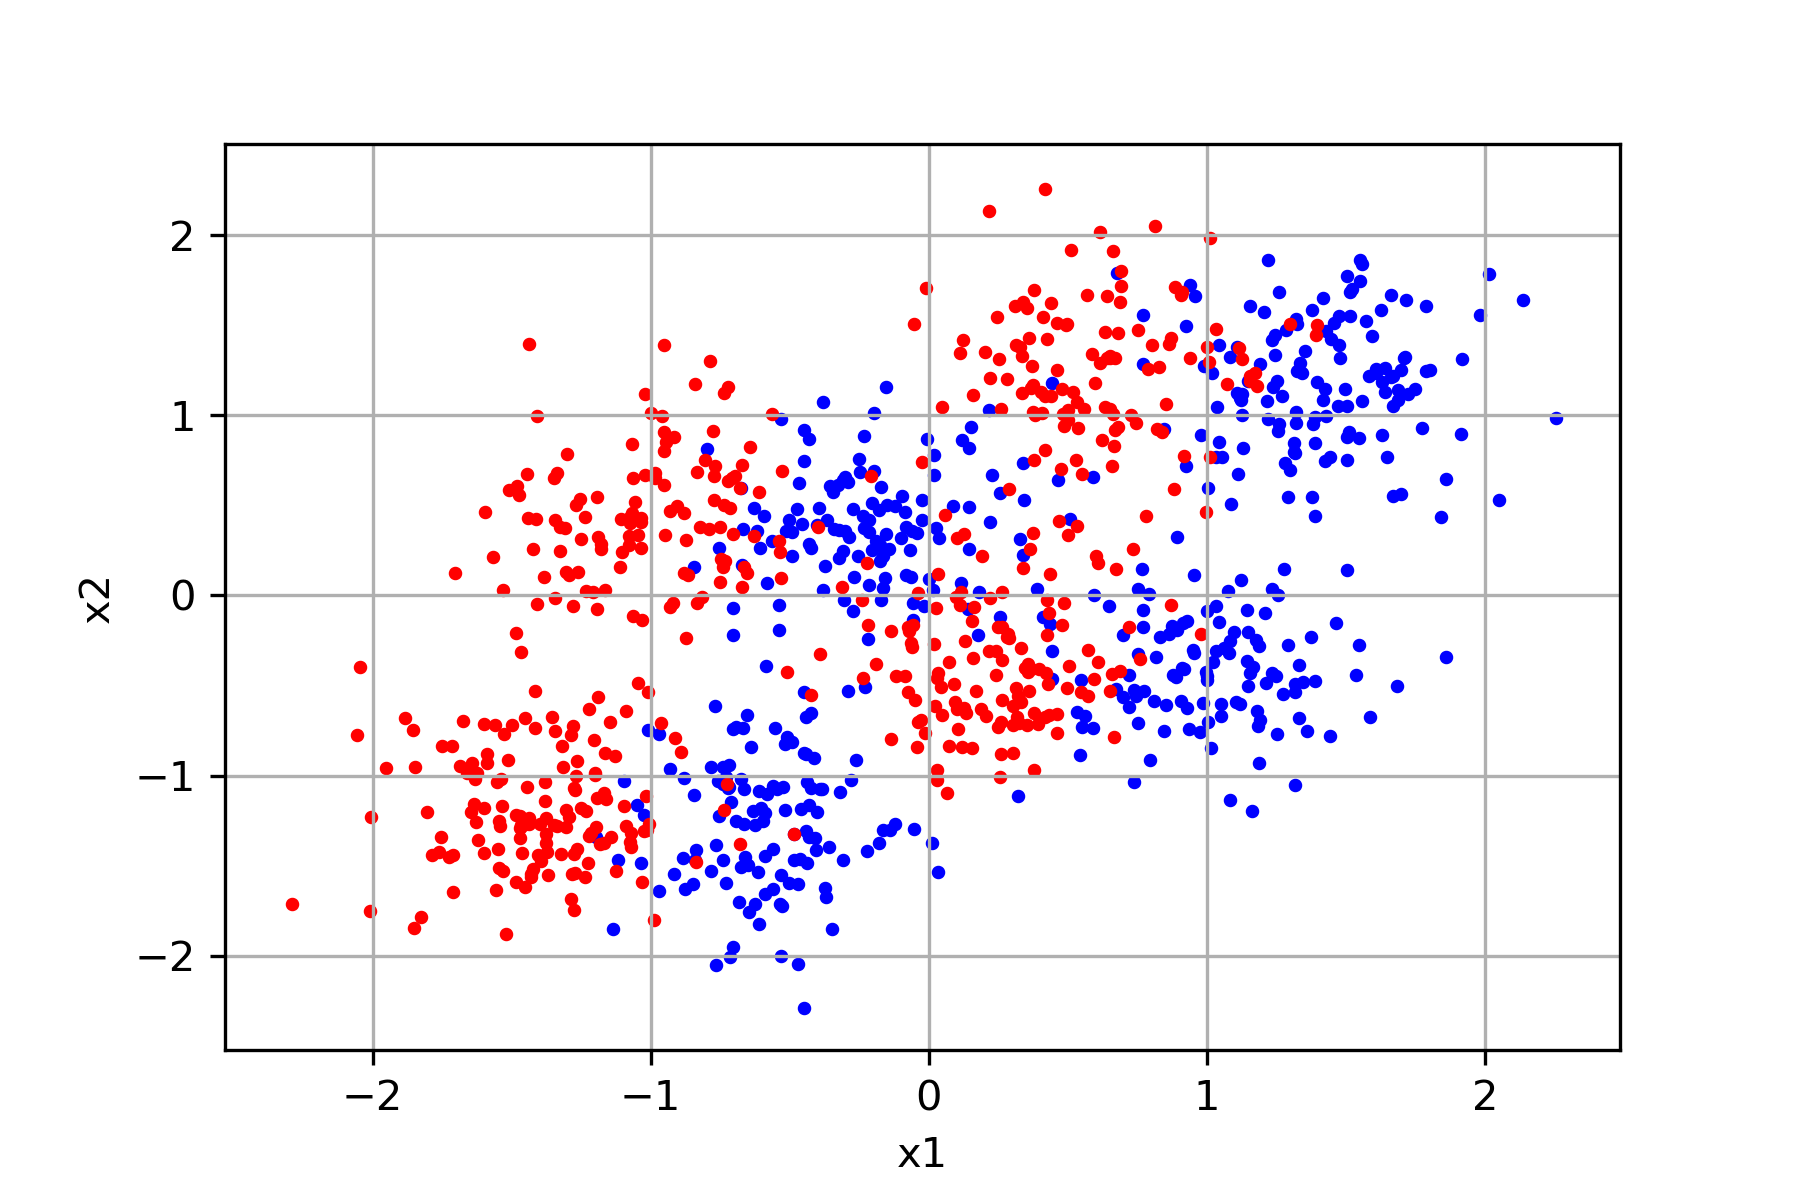
\includegraphics[width=12cm]{raw_data}
    \caption{Training set}
    \label{fig:mlp-raw_data}
\end{figure}

\begin{figure}[H]
    \centering
    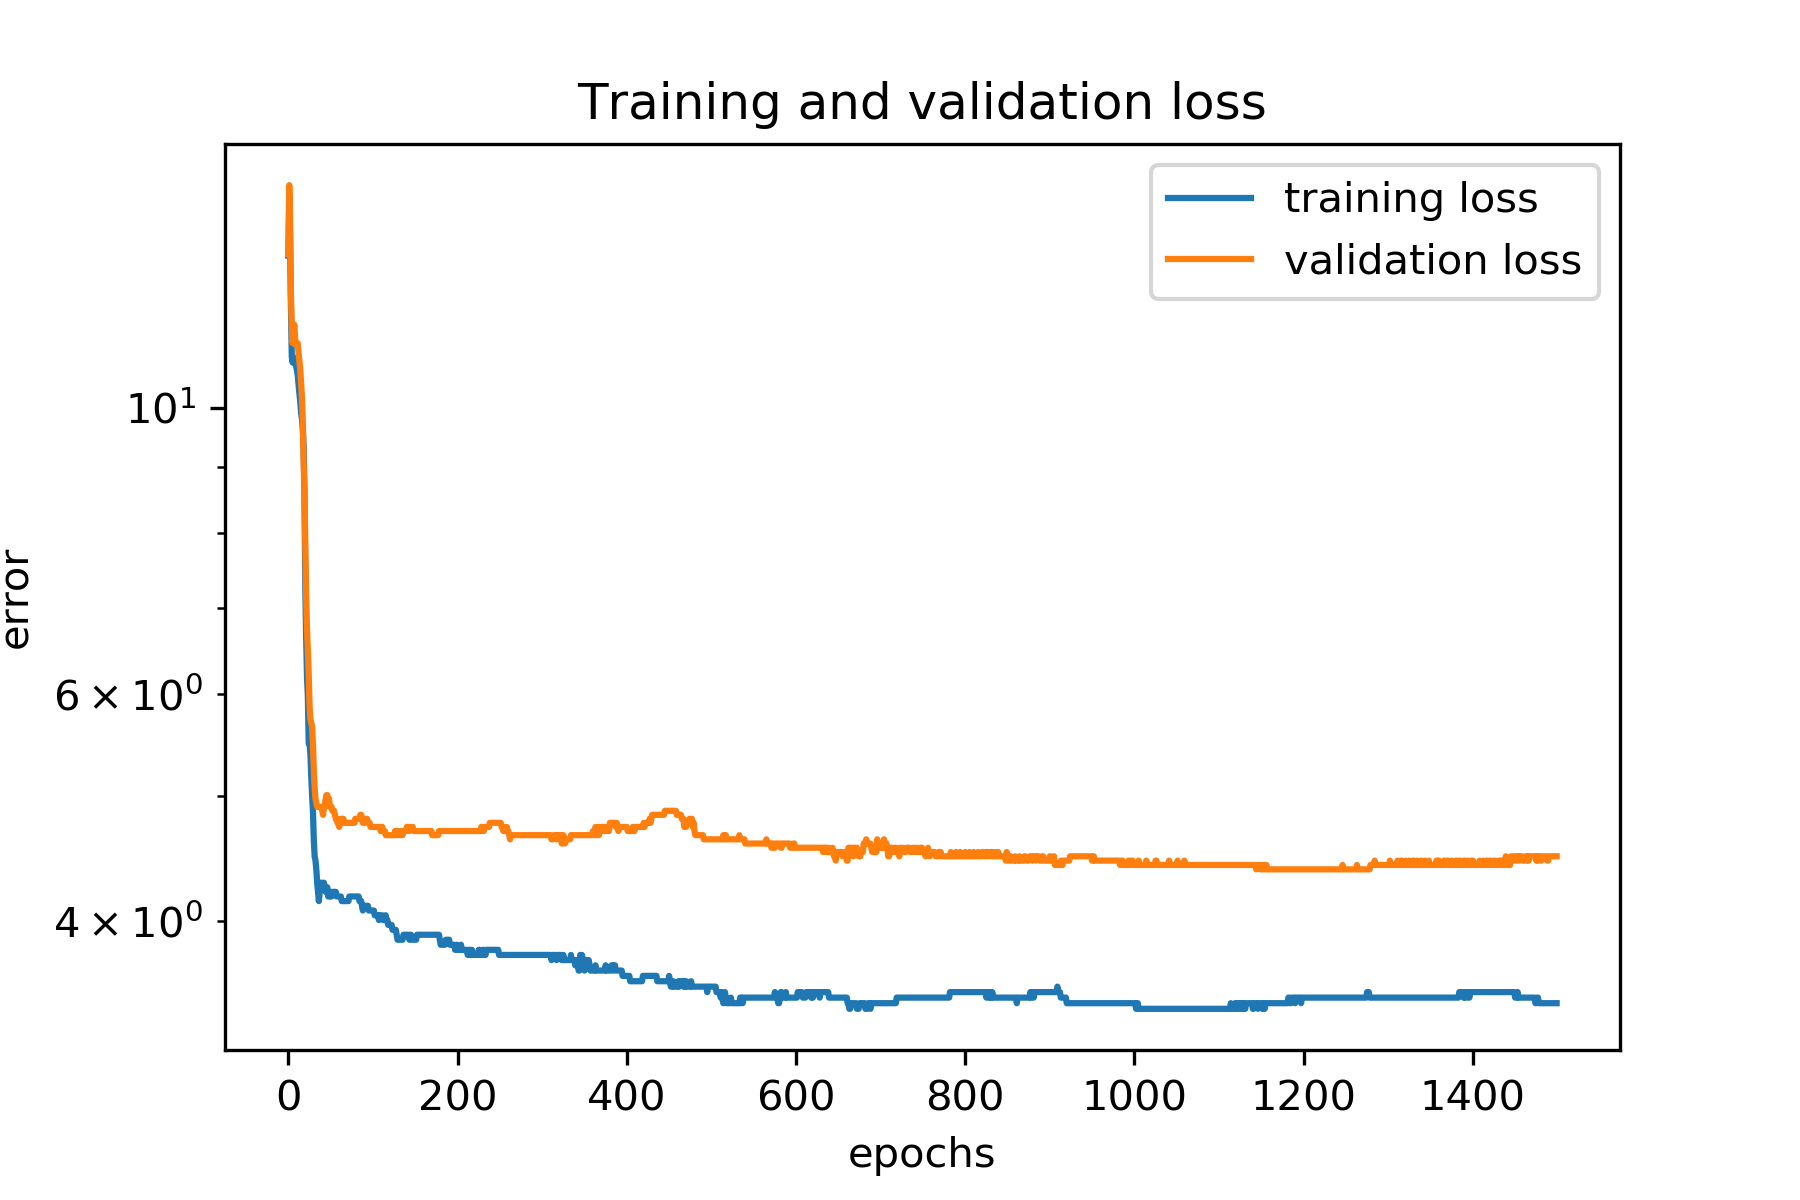
\includegraphics[width=12cm]{training_validation_loss}
    \caption{Progression of cost function in training and validation}
    \label{fig:mlp-training_validation_loss}
\end{figure}

\paragraph{In Figure \ref{fig:mlp-roc_curve} we can see the ROC curve for this classifier.}

\begin{figure}[H]
    \centering
    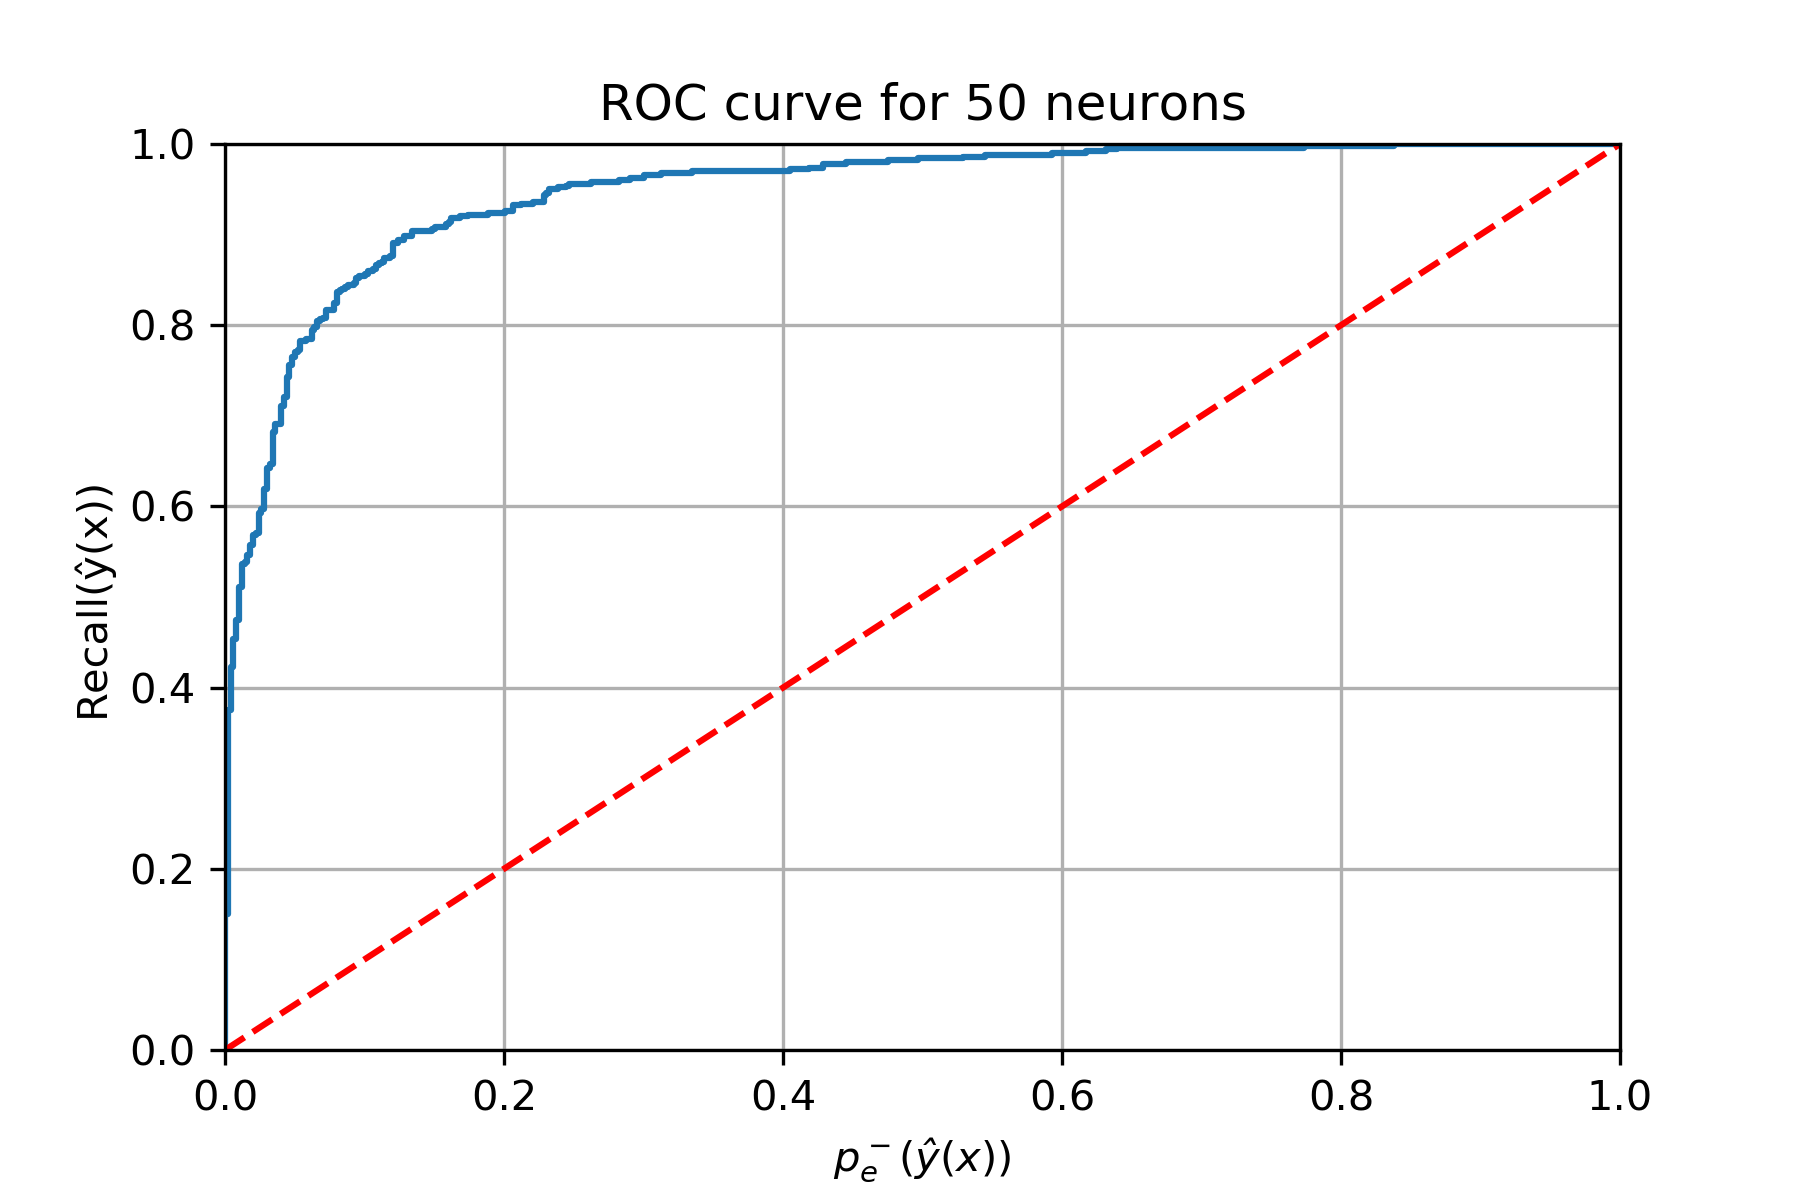
\includegraphics[width=12cm]{ROC_curve}
    \caption{ROC curve for 50 neurons}
    \label{fig:mlp-roc_curve}
\end{figure}

%--------------------------------------
\subsubsection{b) MLP decision regions}
%--------------------------------------

\paragraph{A function was created to plot the decision regions. This function receives as parameters the dataset and the model. The dataset is used only to define the limits of the plot and the predict method of the model is used to determine the label of each division of the grid. The Figure \ref{fig:mlp-decision_regions} shows the decision regions for this MLP classifier.}

\begin{figure}[H]
    \centering
    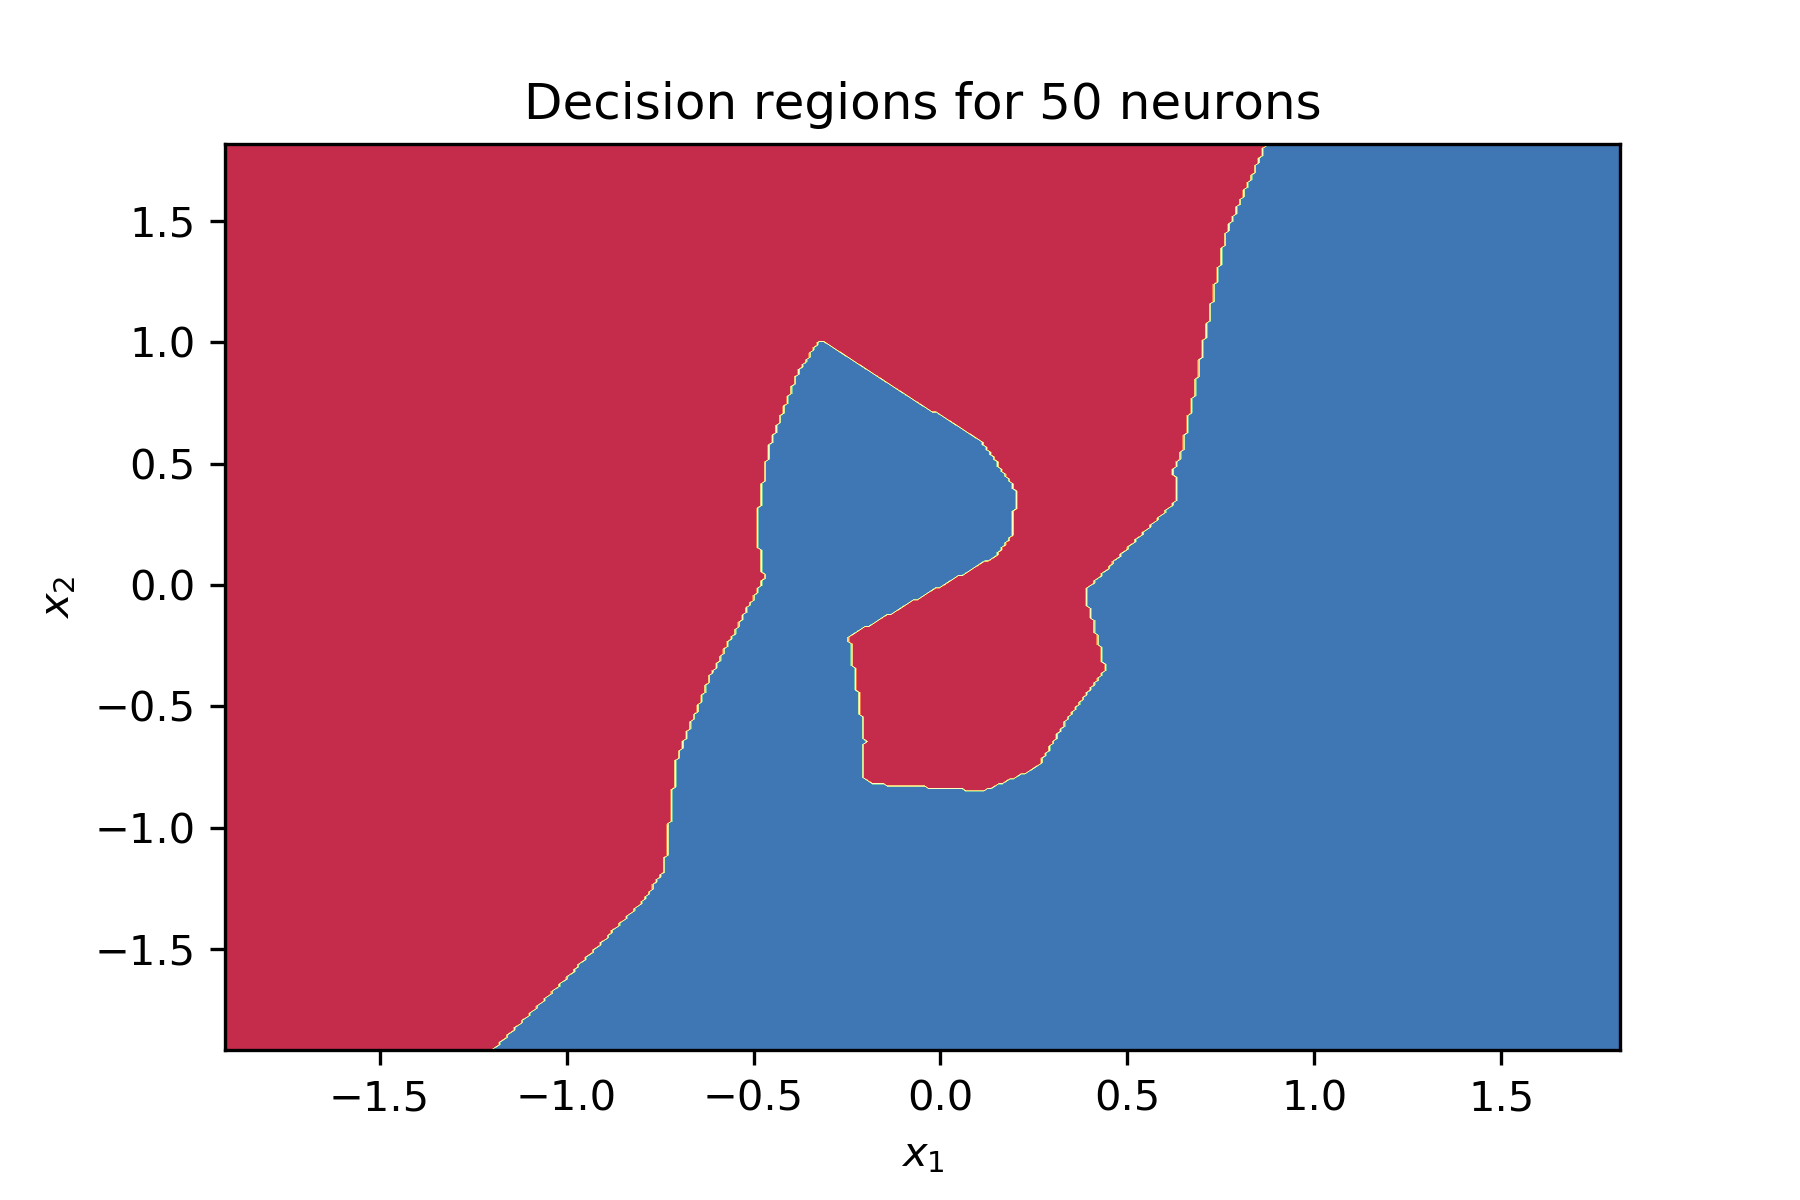
\includegraphics[width=12cm]{mlp_decision_region}
    \caption{Decision regions for MLP with 50 neurons}
    \label{fig:mlp-decision_regions}
\end{figure}

%--------------------------------------
\subsubsection{c) Applying MLP model to test set}
%--------------------------------------

\paragraph{We then applied the trained network in the test set. The output generated can be seen in Figure \ref{fig:mlp-test_set_output}. The accuracy was 0.879, indicating an error of 12.1\%.}

\begin{figure}[H]
    \centering
    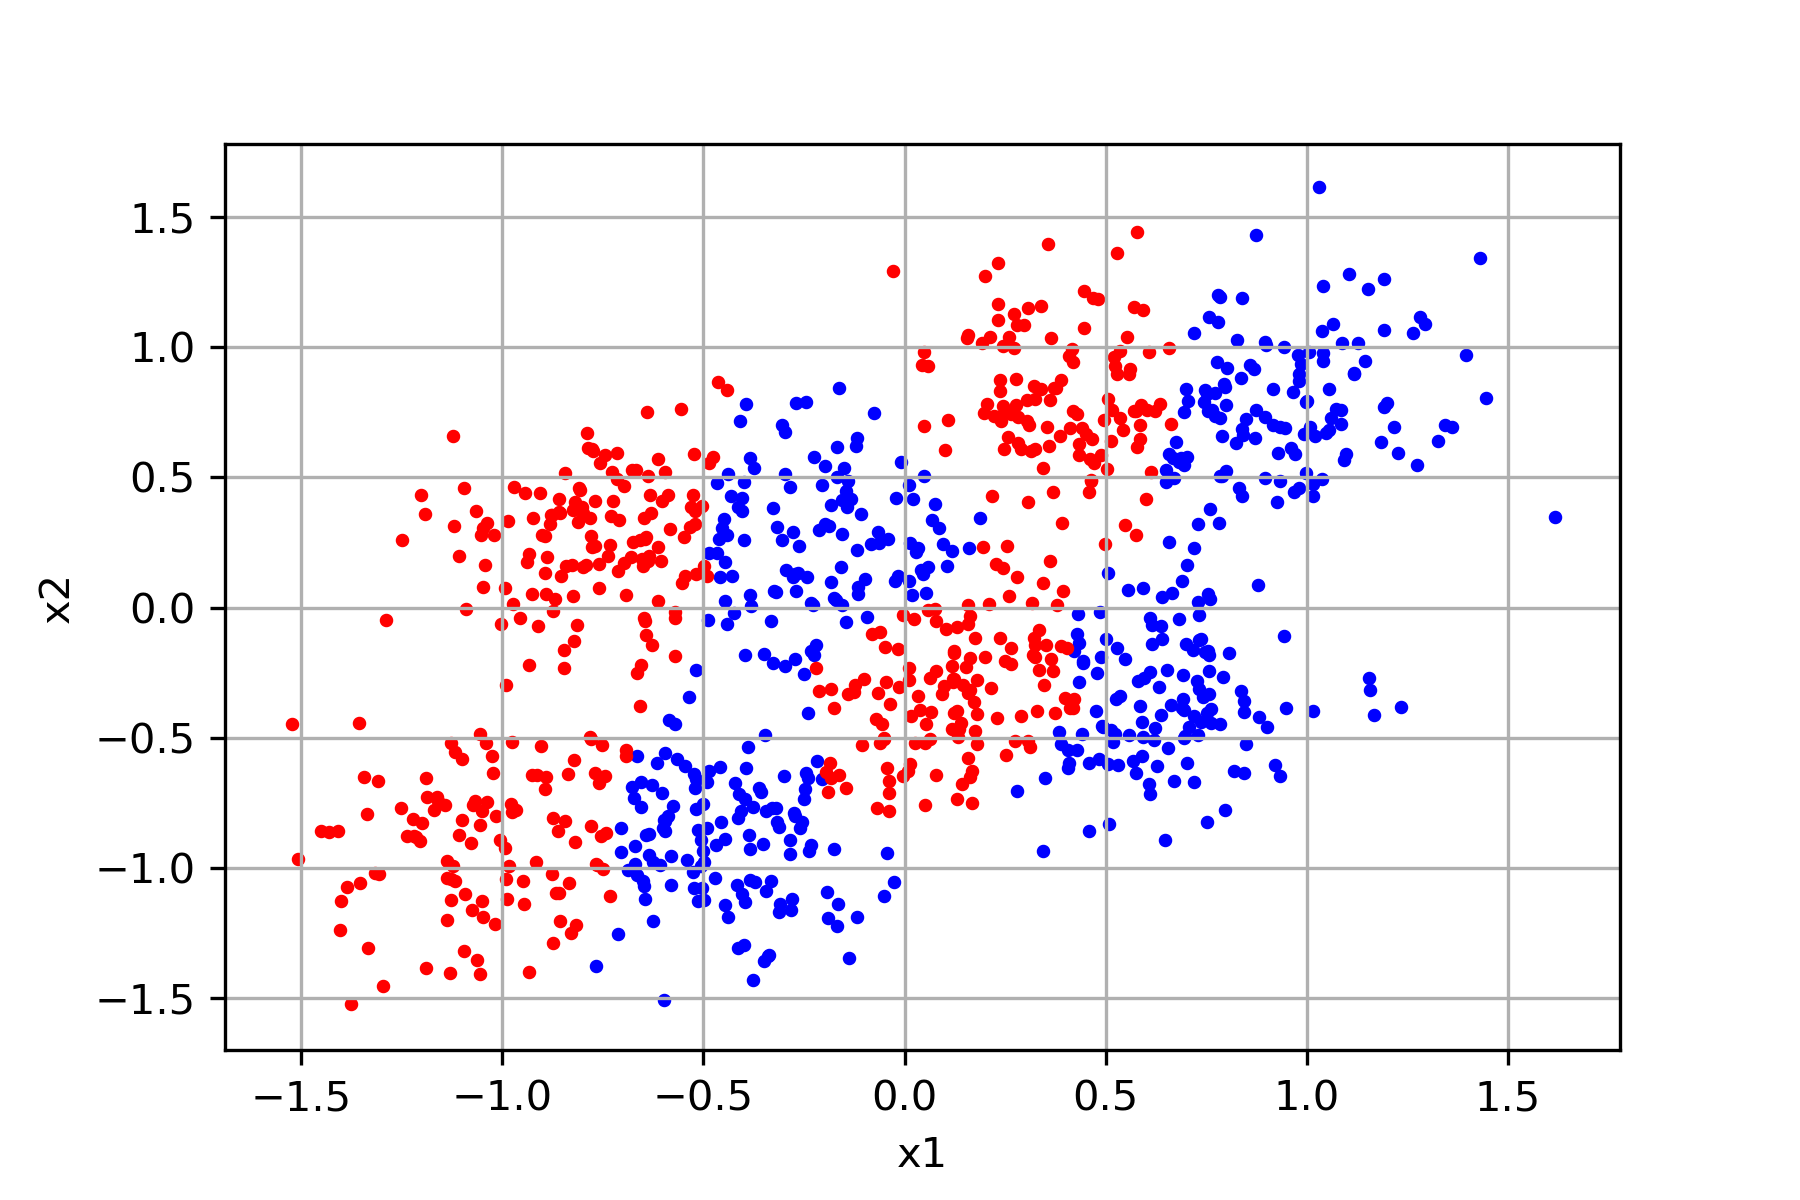
\includegraphics[width=12cm]{mlp_test_set_output}
    \caption{MLP predicted output for test set}
    \label{fig:mlp-test_set_output}
\end{figure}

%--------------------------------------
\subsubsection{d) Experimenting network with different number of neurons}
%--------------------------------------

\paragraph{We then tried networks with different number of neurons. 5, 25, 75, 100, 300, 1000 and 5000 neurons were utilized. Figure \ref{fig:mlp-decision_regions_N_neurons} shows the decisions regions for these classifiers and Figure \ref{fig:mlp-ROC_N_neurons} shows the ROC curves.}

%-------------------------------------------------
%\newpage
% decision regions for different number of neurons

\begin{figure}[H]
    \centering
    % 5 neurons
    \begin{subfigure}{0.32\textwidth}
        \centering
        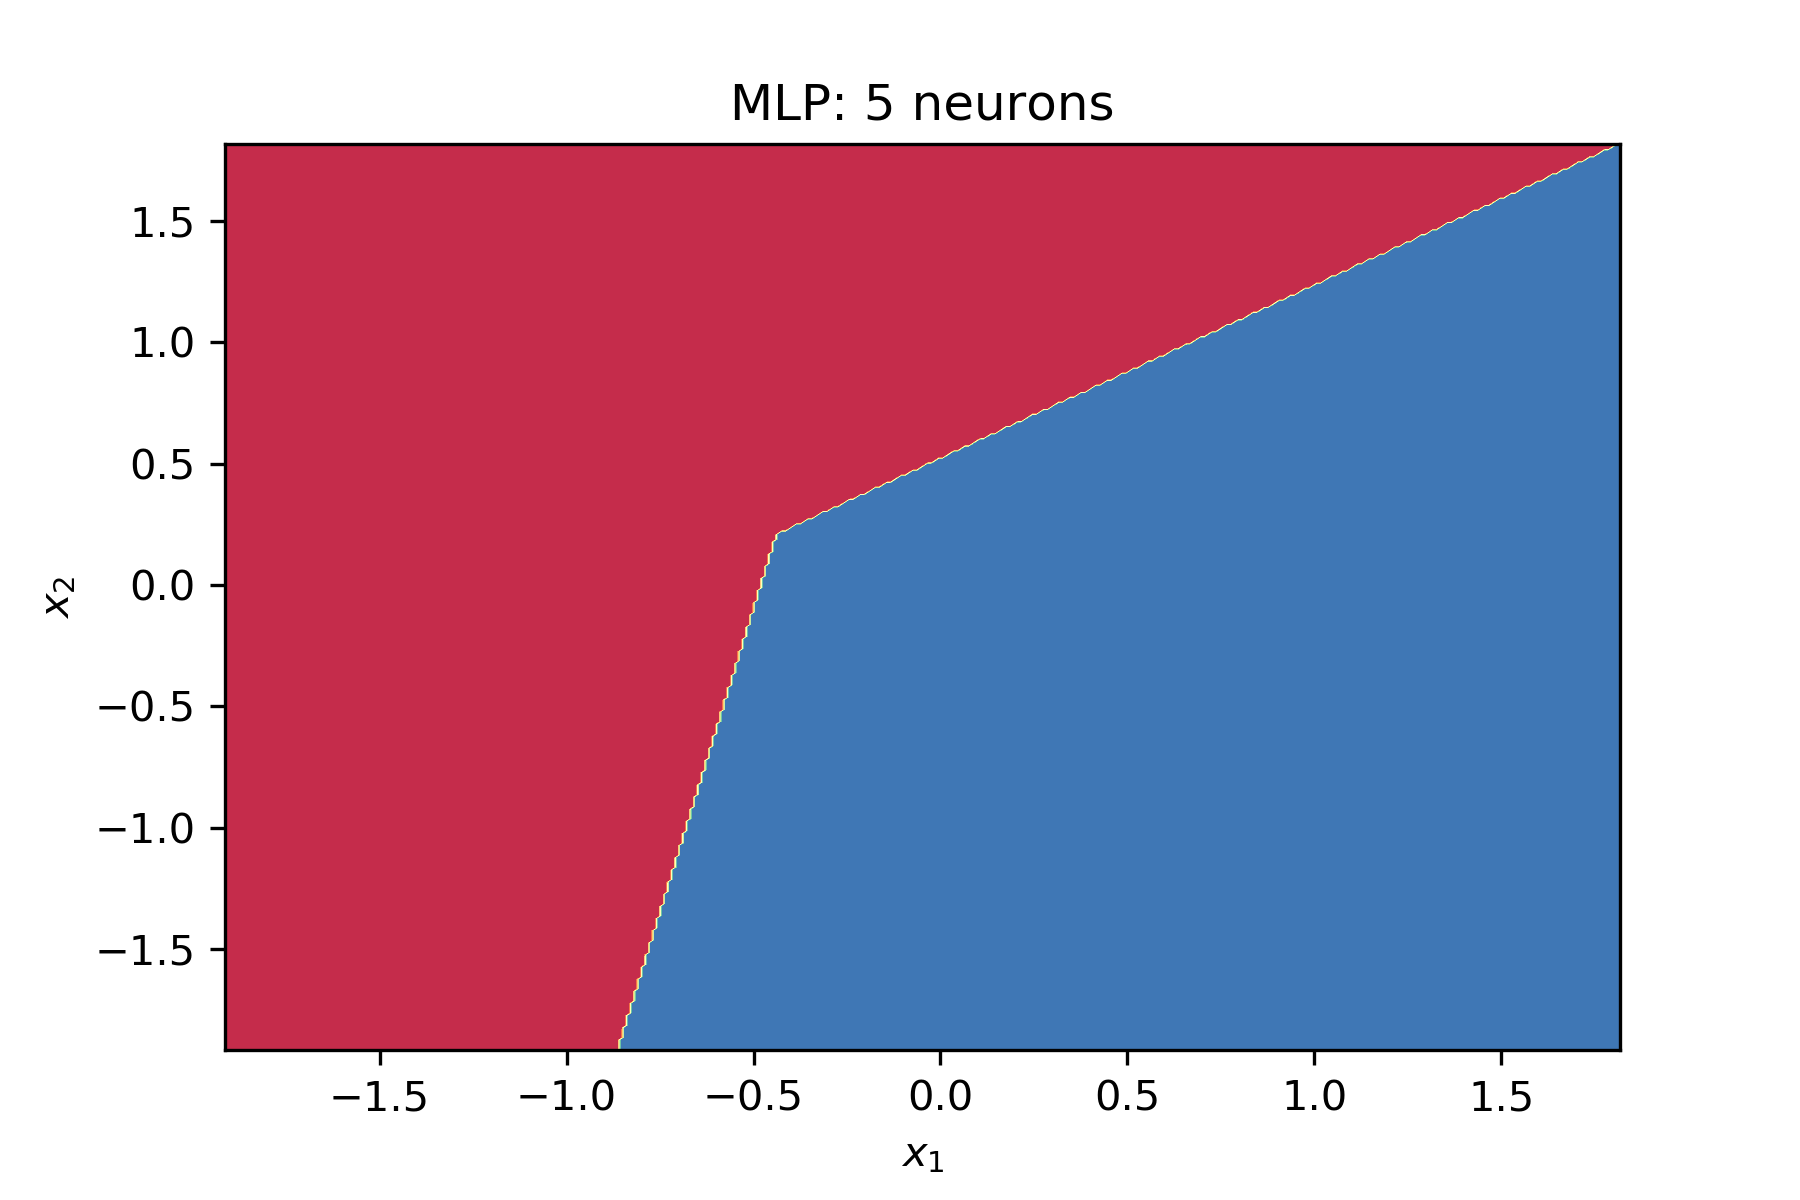
\includegraphics[width=3.85cm]{decision_regions_5}
        \caption{5 neurons}
        \label{fig:mlp-5_neurons}
    \end{subfigure}
    \hfill
    % 25 neurons
    \begin{subfigure}{0.32\textwidth}
        \centering
        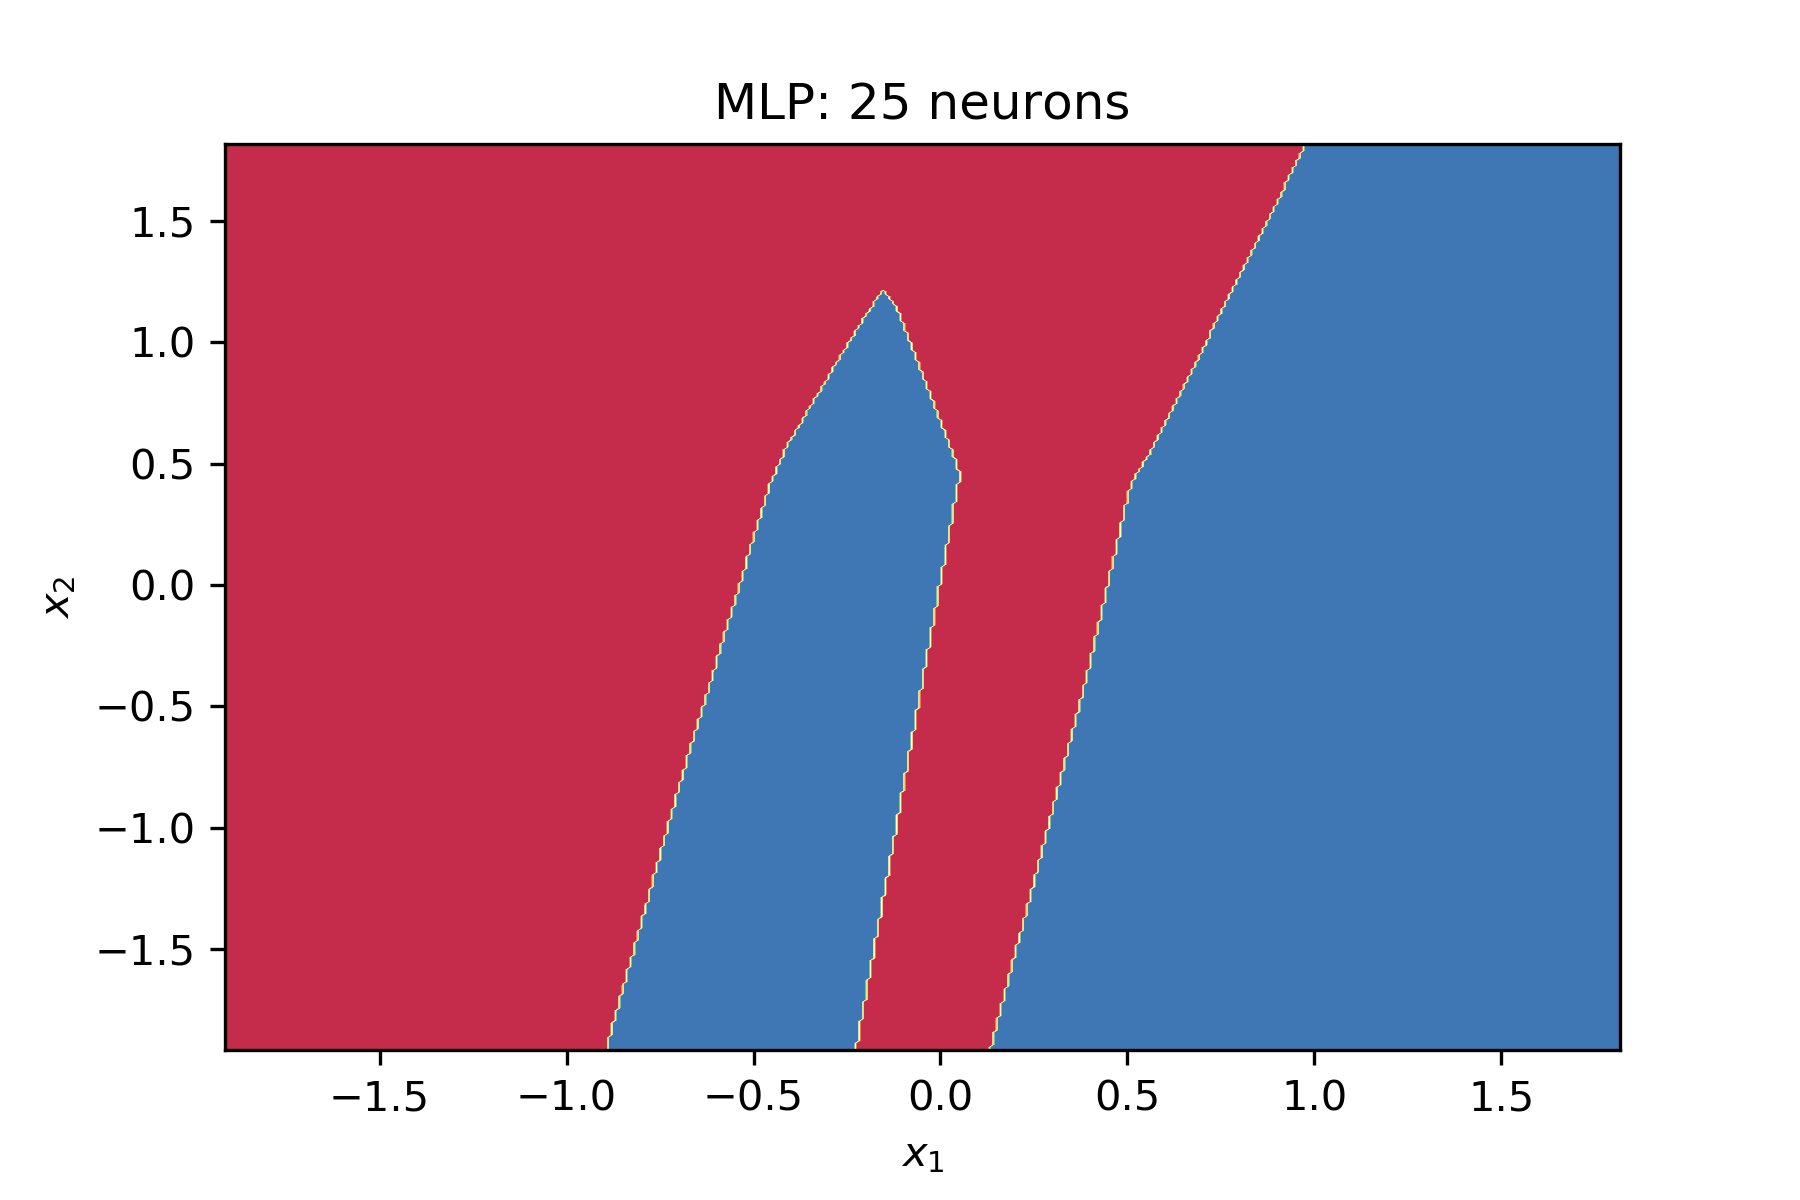
\includegraphics[width=3.85cm]{decision_regions_25}
        \caption{25 neurons}
        \label{fig:mlp-25_neurons}
    \end{subfigure}
    \hfill
    % 75 neurons
    \begin{subfigure}{0.32\textwidth}
        \centering
        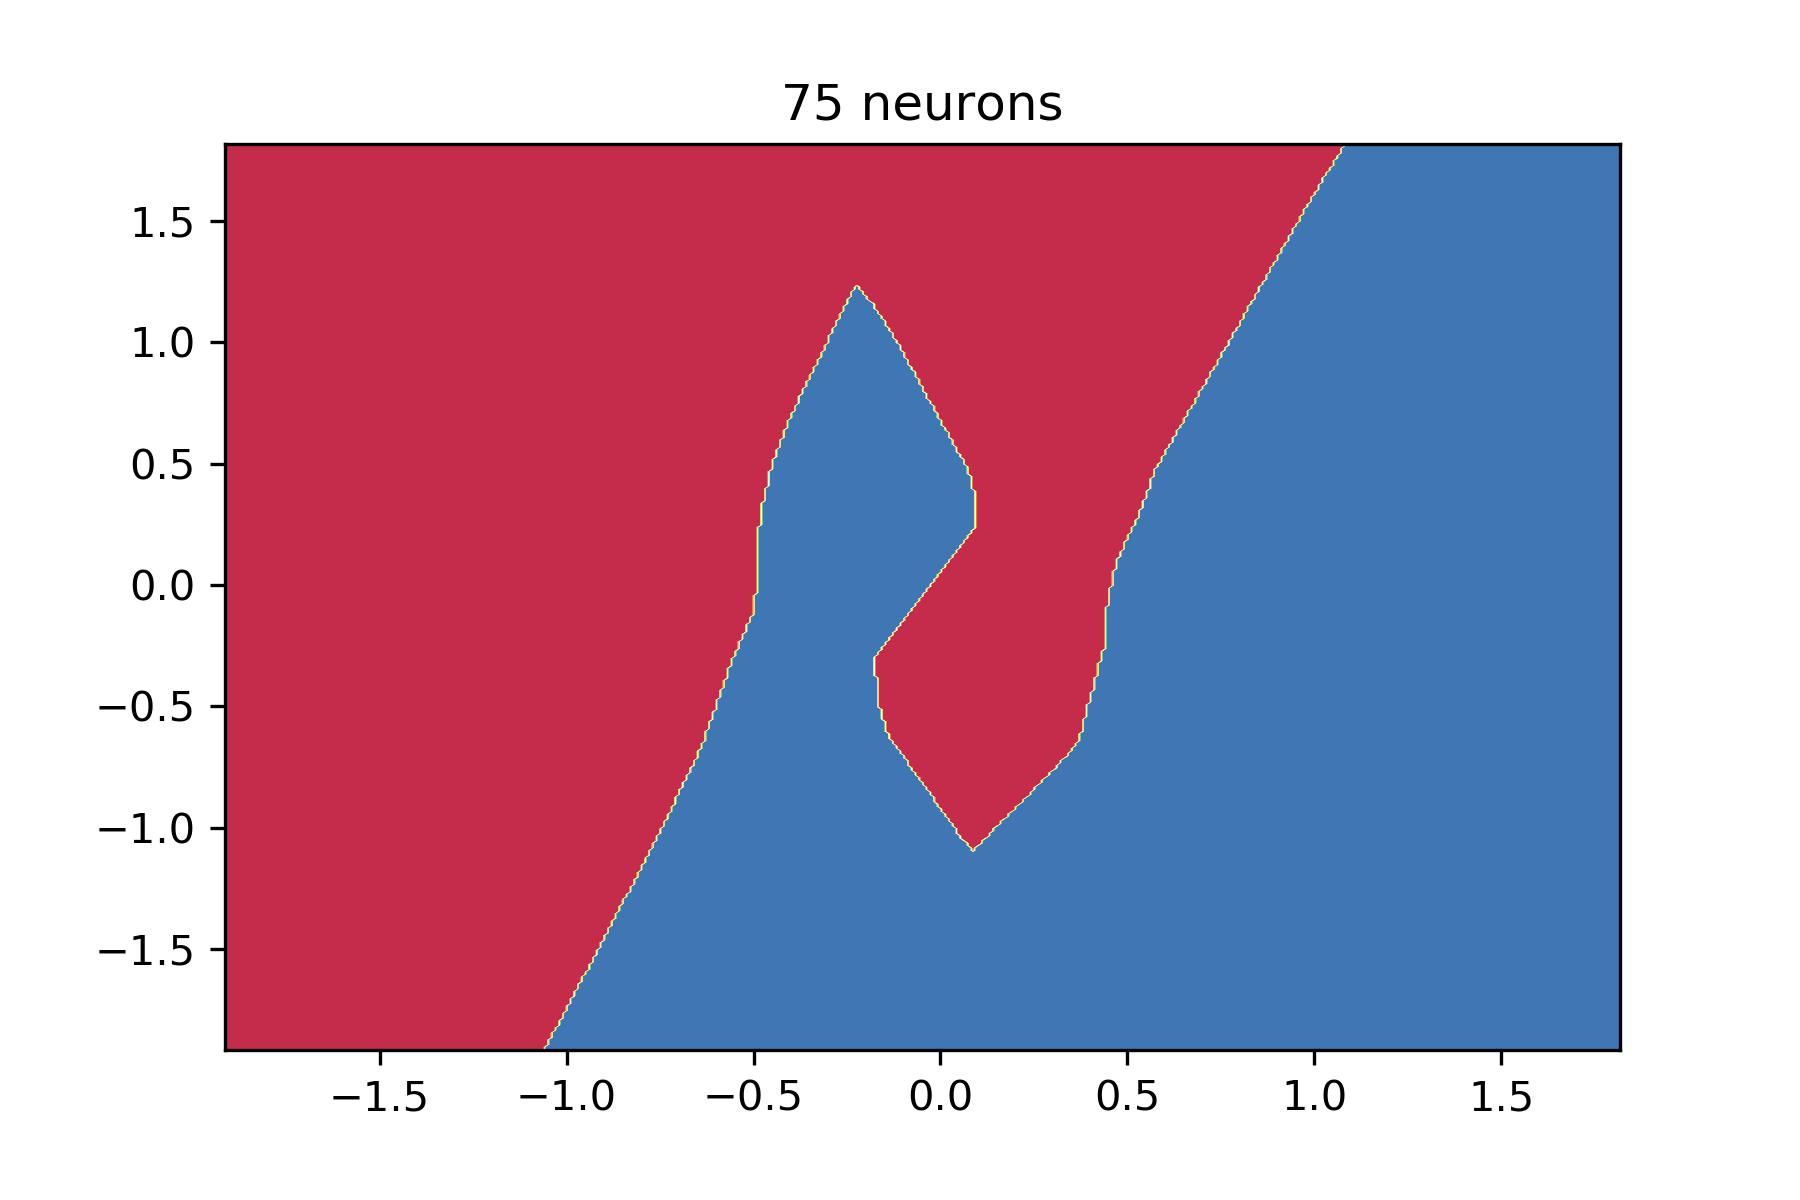
\includegraphics[width=3.85cm]{decision_regions_75}
        \caption{75 neurons}
        \label{fig:mlp-75_neurons}
    \end{subfigure}
    \hfill
    % 100 neurons
    \begin{subfigure}{0.32\textwidth}
        \centering
        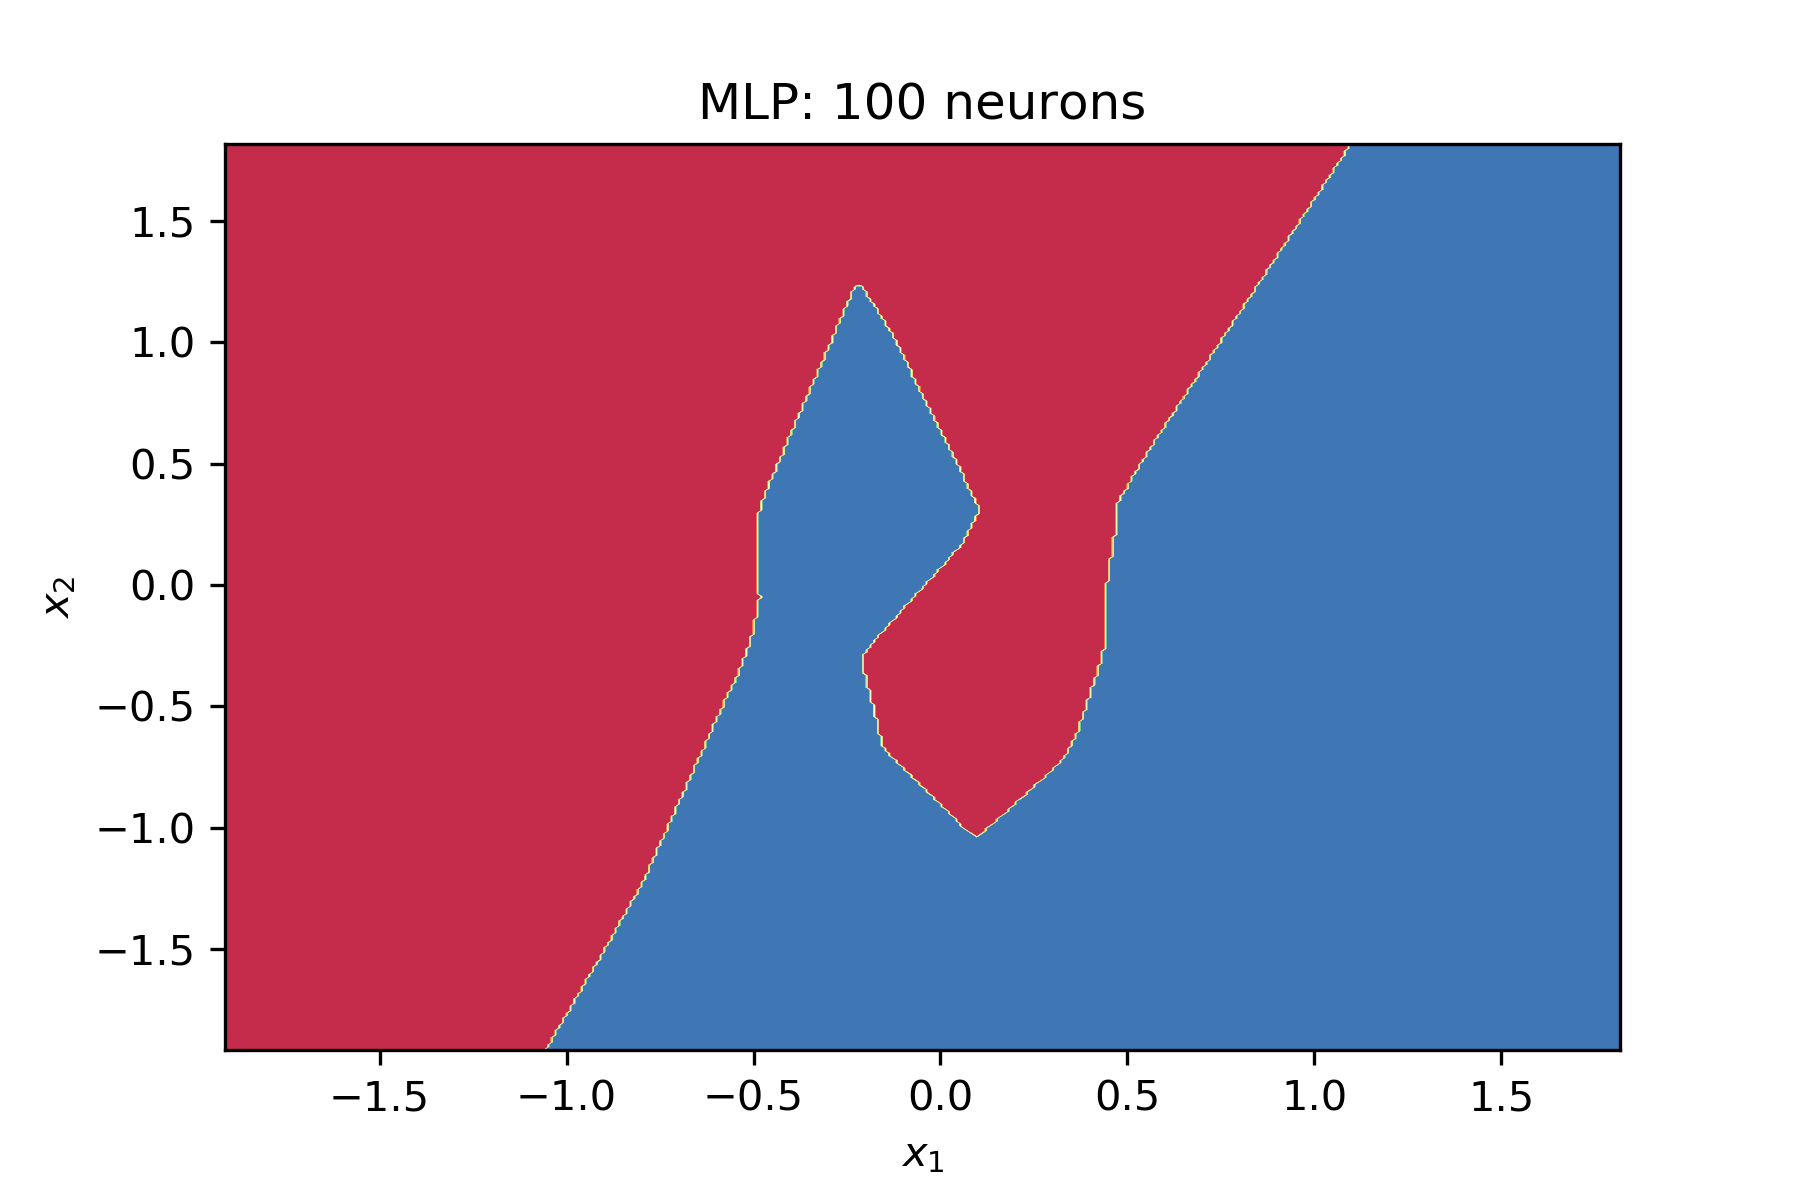
\includegraphics[width=3.85cm]{decision_regions_100}
        \caption{100 neurons}
        \label{fig:mlp-100_neurons}
    \end{subfigure}
    \hfill
    % 300 neurons
    \begin{subfigure}{0.32\textwidth}
        \centering
        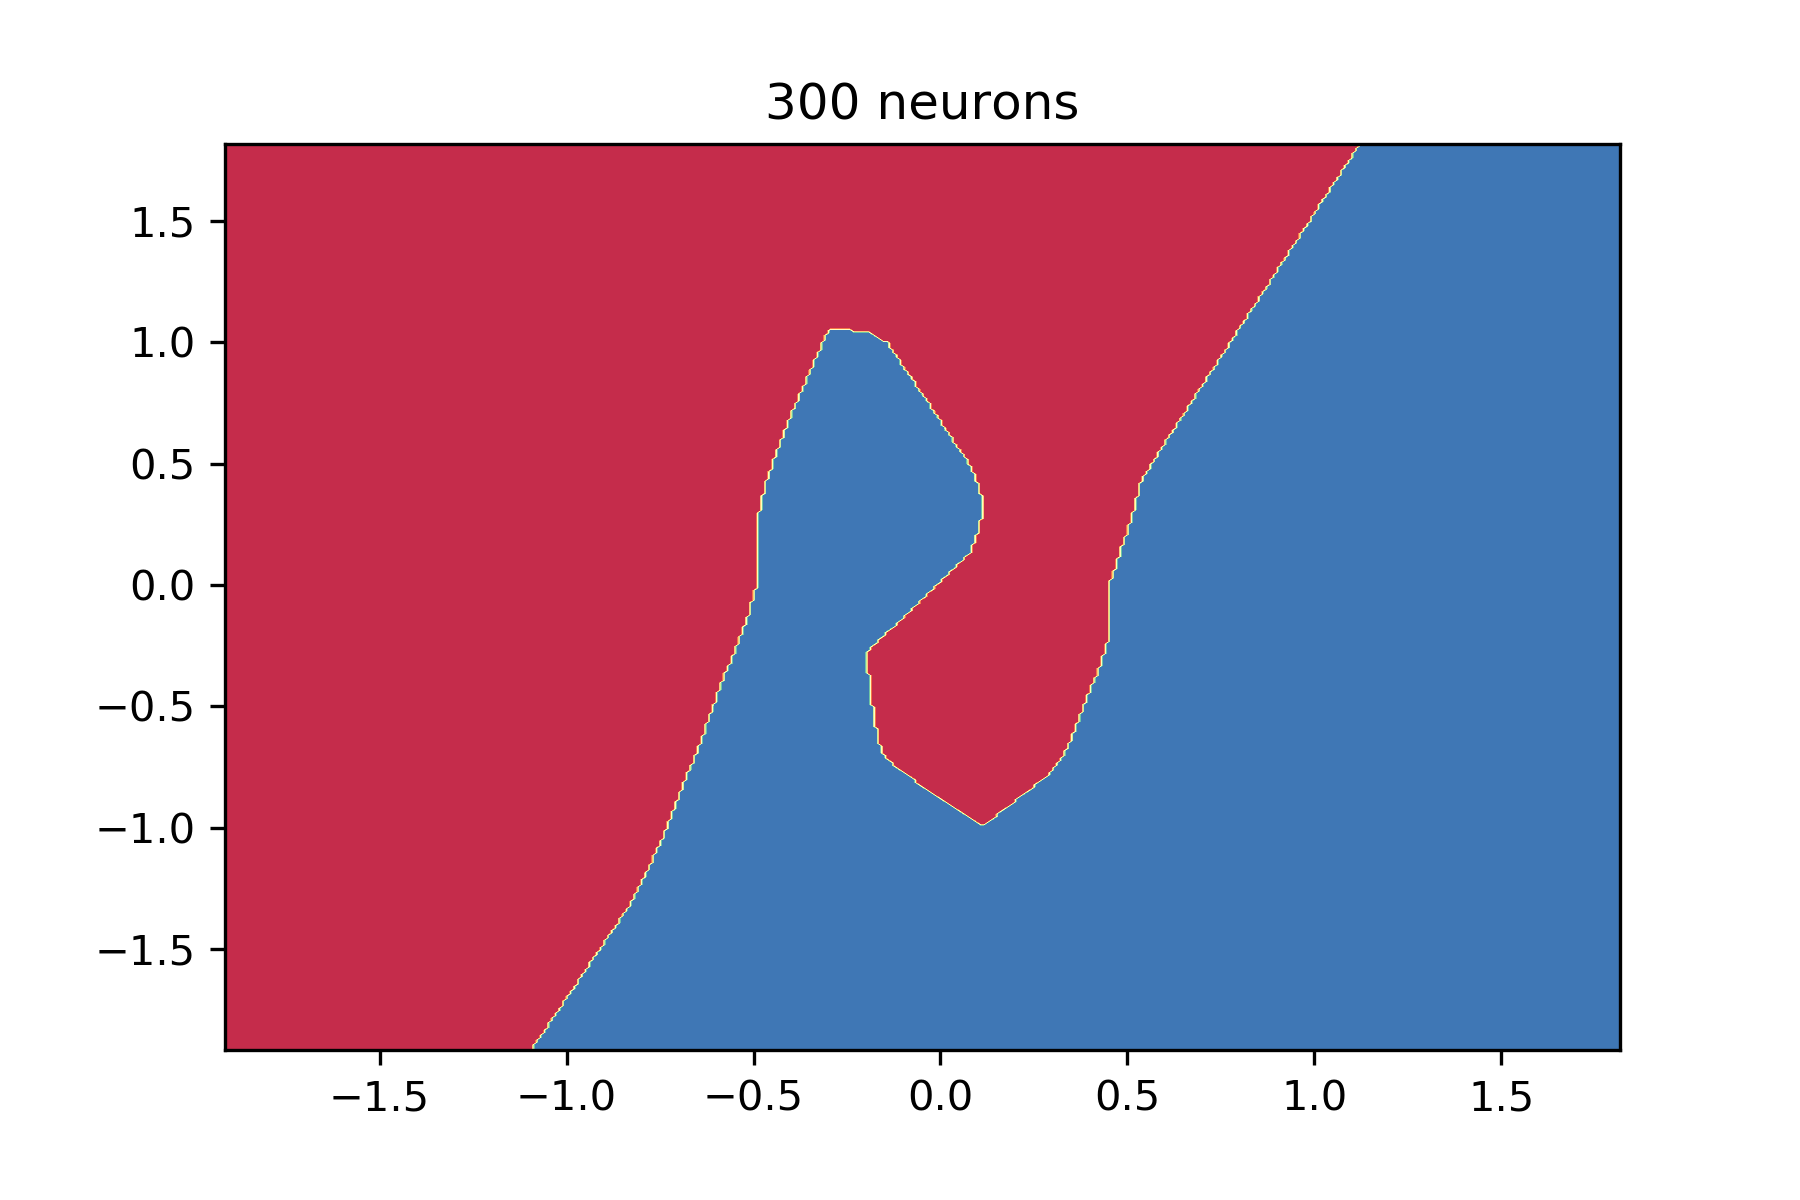
\includegraphics[width=3.85cm]{decision_regions_300}
        \caption{300 neurons}
        \label{fig:mlp-300_neurons}
    \end{subfigure}
    \hfill
    % 1000 neurons
    \begin{subfigure}{0.32\textwidth}
        \centering
        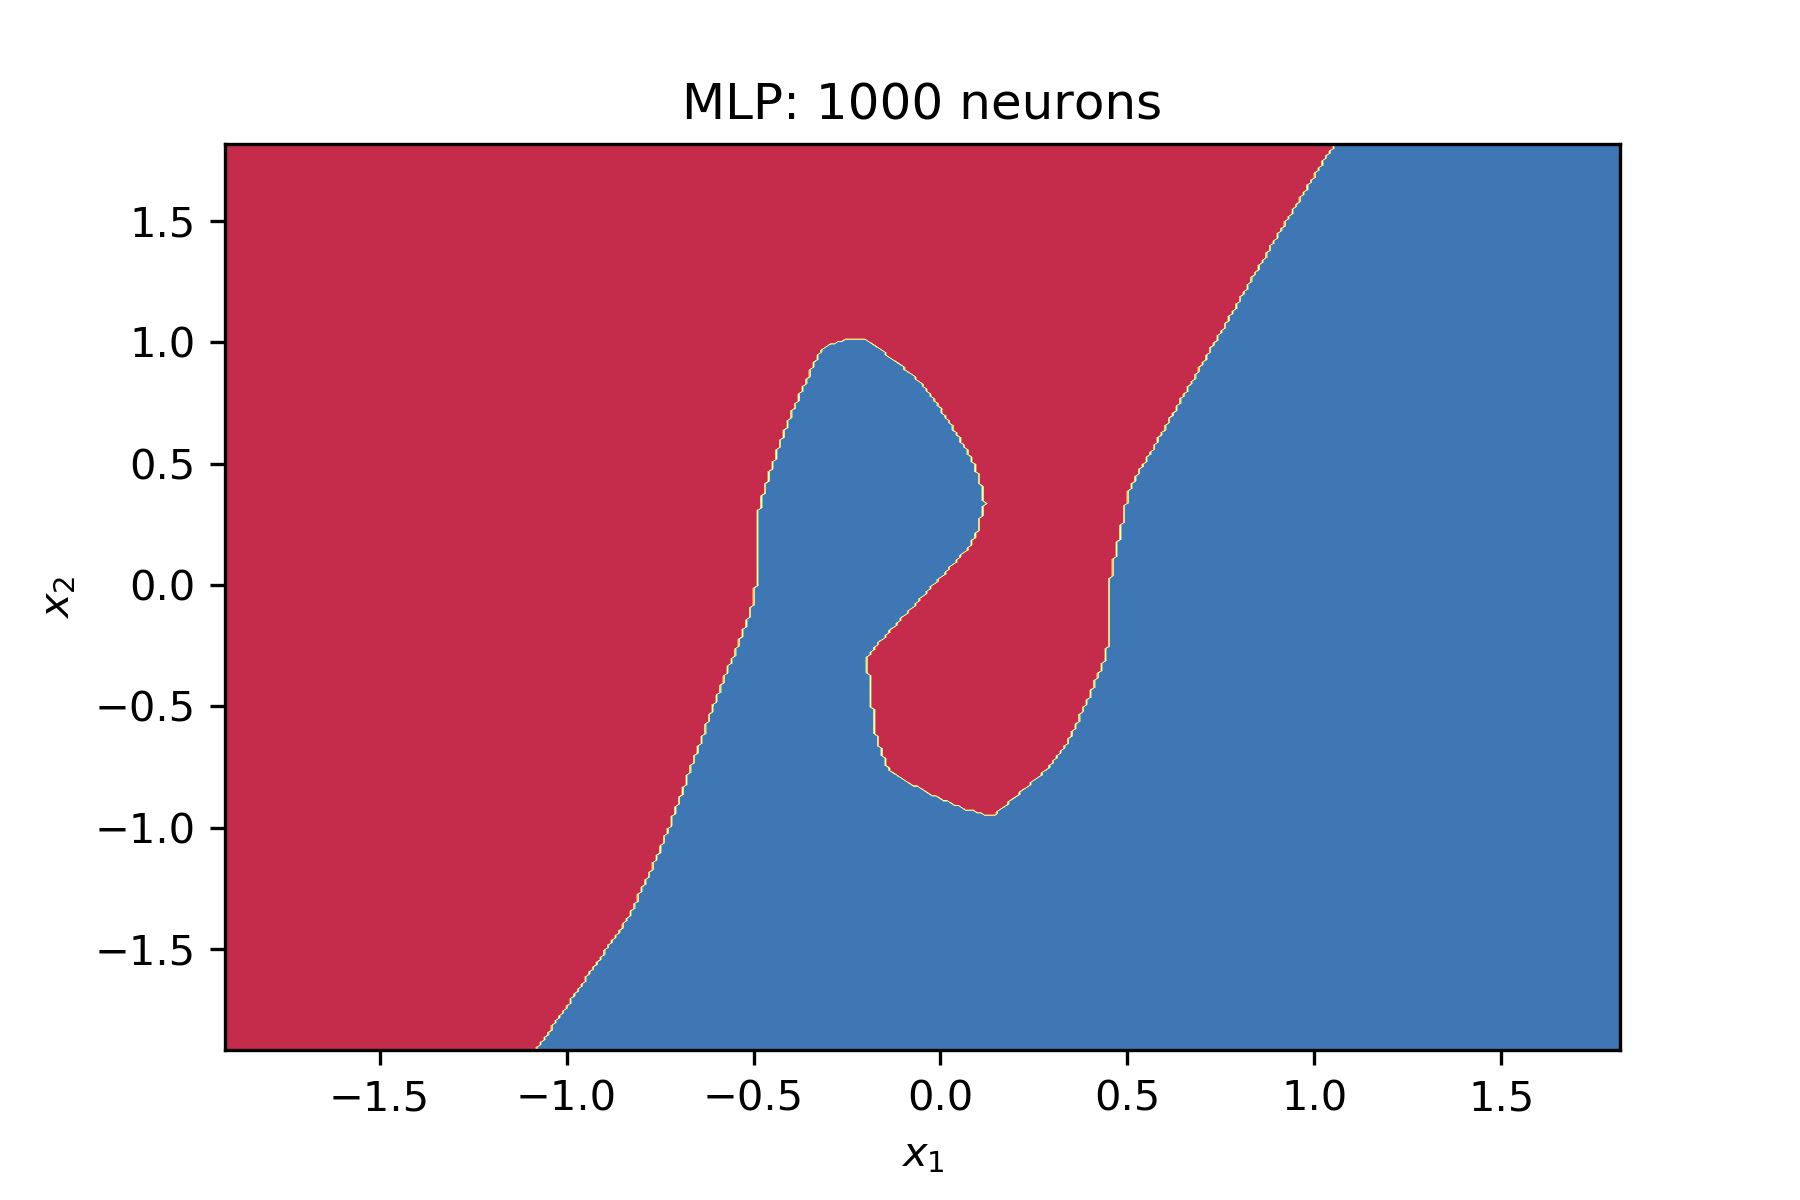
\includegraphics[width=3.85cm]{decision_regions_1000}
        \caption{1000 neurons}
        \label{fig:mlp-1000_neurons}
    \end{subfigure}
    \hfill
    % 5000 neurons
    \begin{subfigure}{0.32\textwidth}
        \centering
        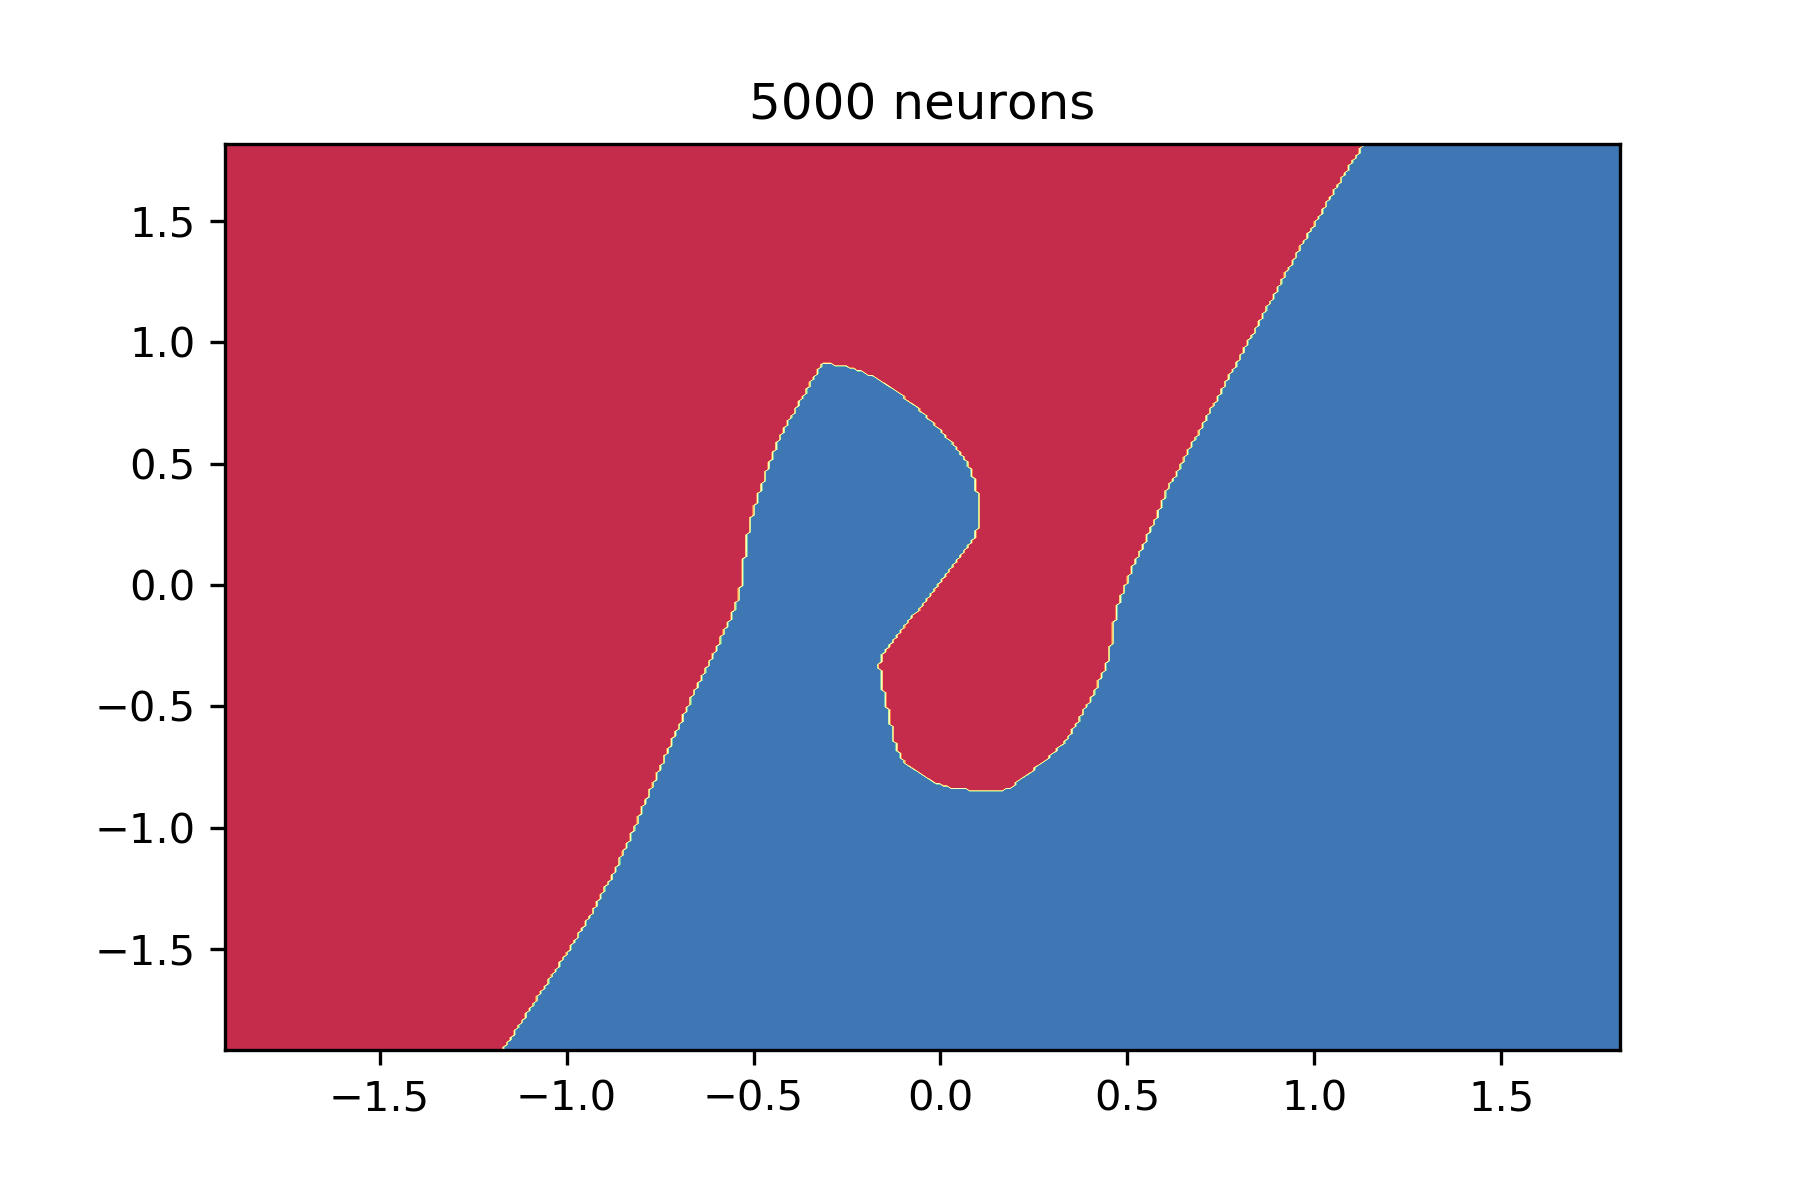
\includegraphics[width=3.85cm]{decision_regions_5000}
        \caption{5000 neurons}
        \label{fig:mlp-5000_neurons}
    \end{subfigure}
    \hfill
    % caption and label
    \caption{Decision regions for MLP with different number of neurons}
    \label{fig:mlp-decision_regions_N_neurons}
\end{figure}
%-------------------------------------------------
%\newpage
% ROC curve for different number of neurons

\begin{figure}[H]
    \centering
    % 5 neurons
    \begin{subfigure}{0.32\textwidth}
        \centering
        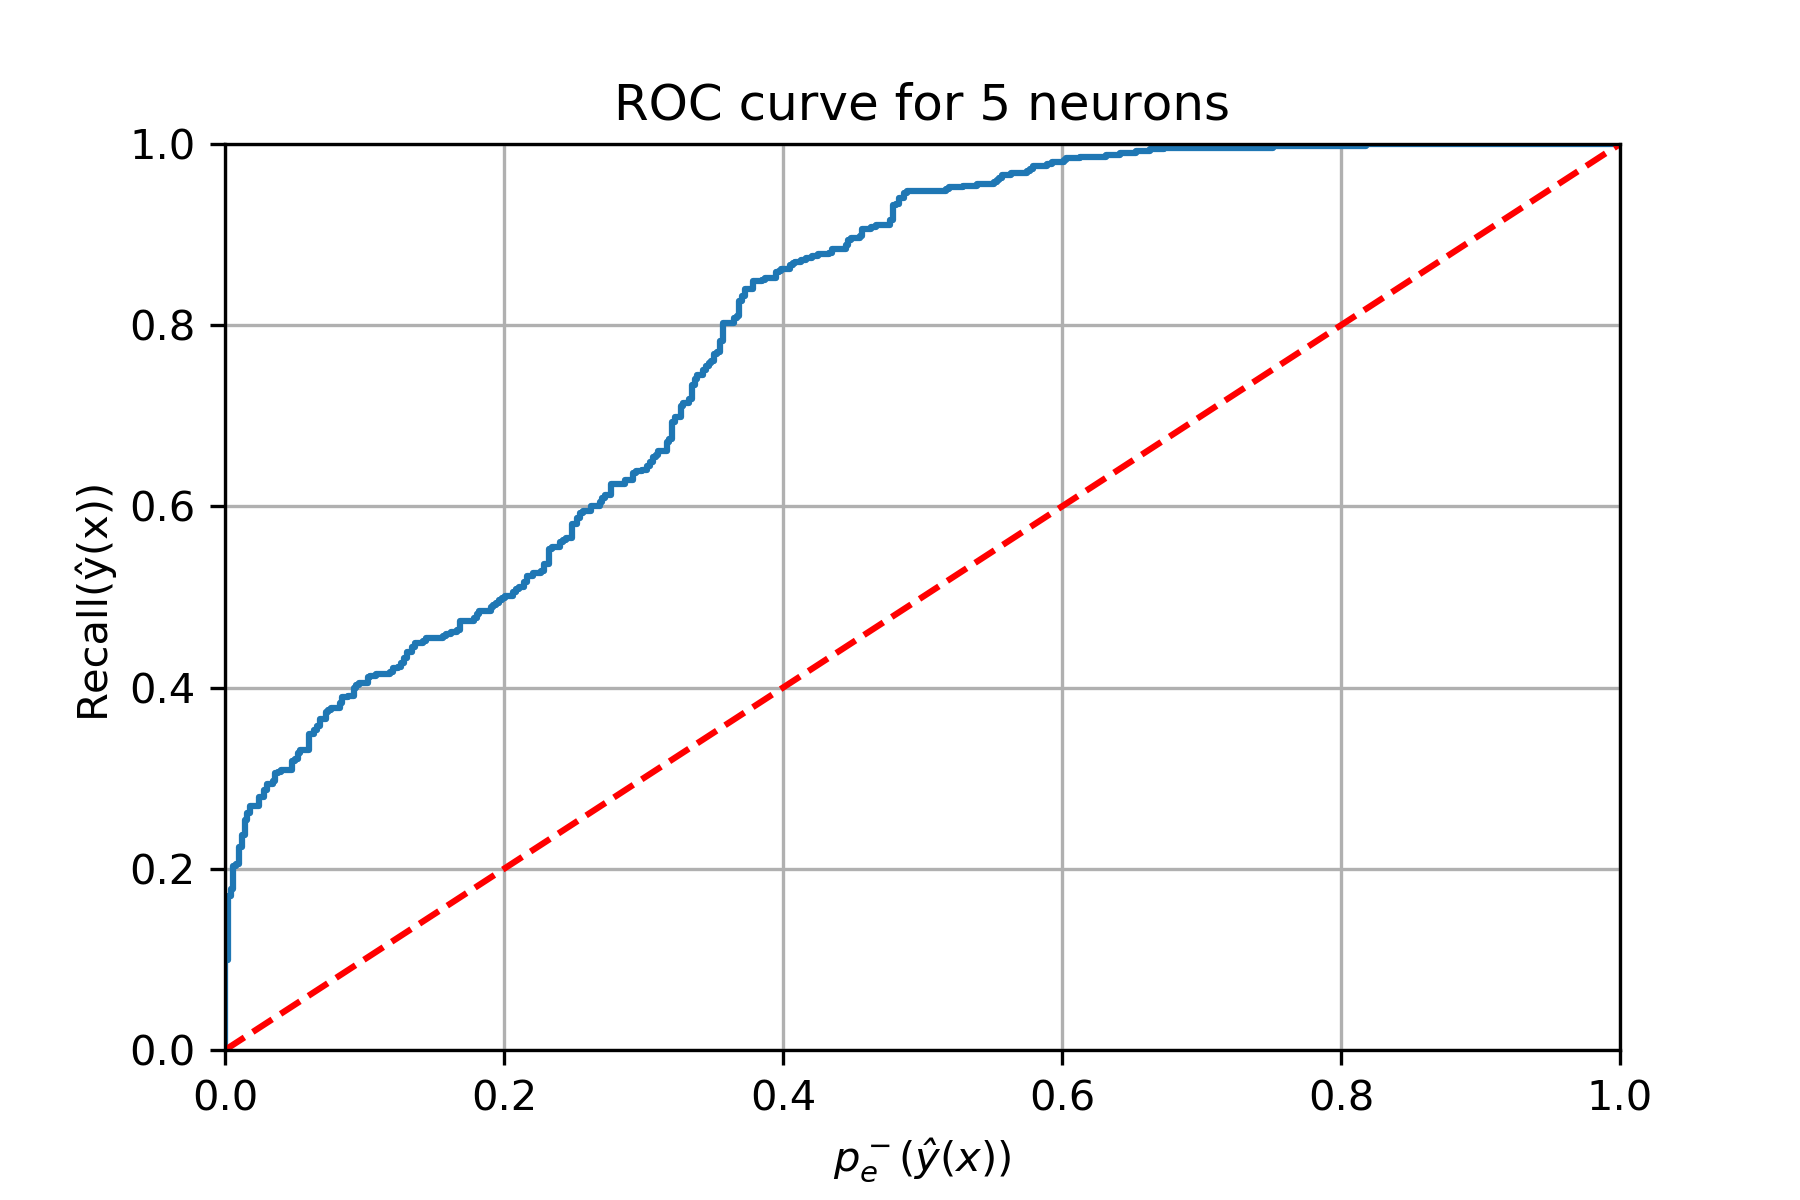
\includegraphics[width=3.85cm]{ROC_5}
        \caption{5 neurons}
        \label{fig:mlp-5_roc}
    \end{subfigure}
    \hfill
    % 25 neurons
    \begin{subfigure}{0.32\textwidth}
        \centering
        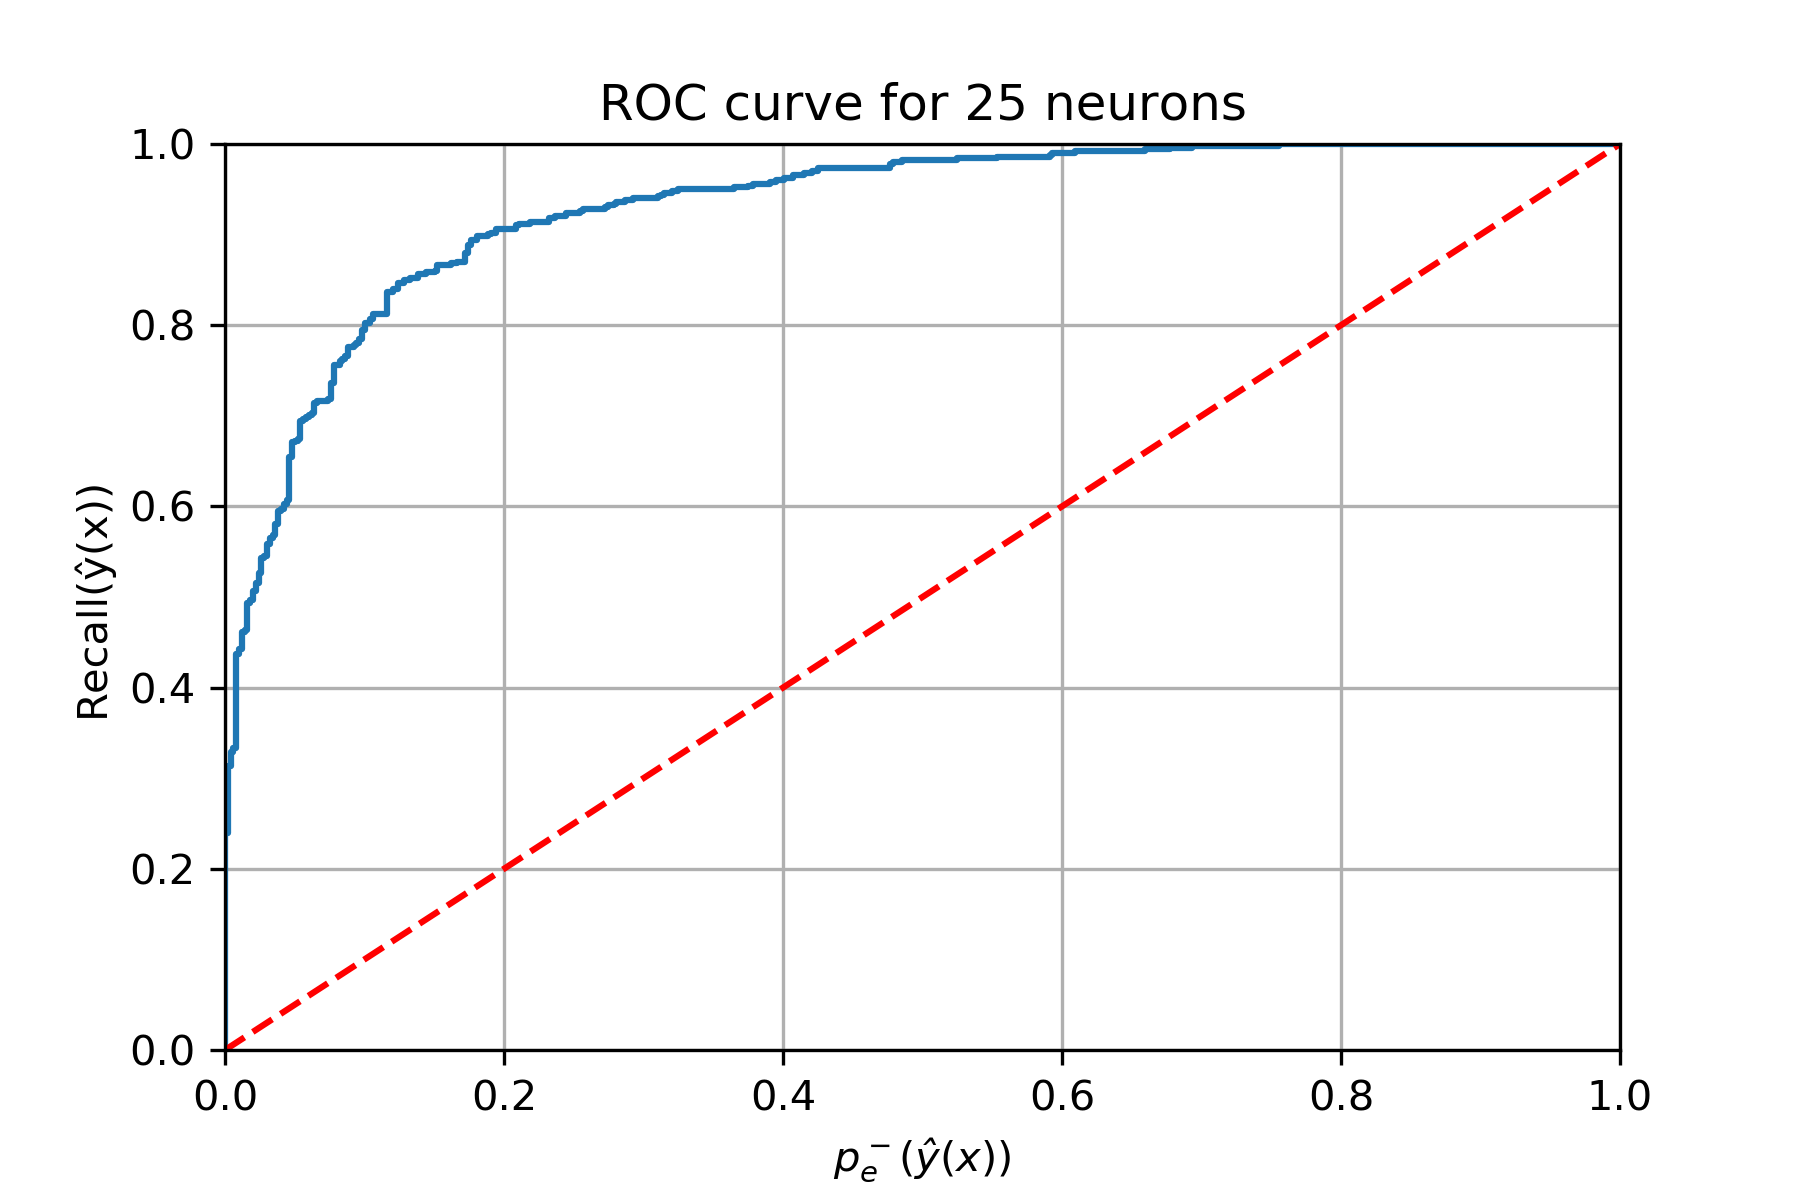
\includegraphics[width=3.85cm]{ROC_25}
        \caption{25 neurons}
        \label{fig:mlp-25_roc}
    \end{subfigure}
    \hfill
    % 75 neurons
    \begin{subfigure}{0.32\textwidth}
        \centering
        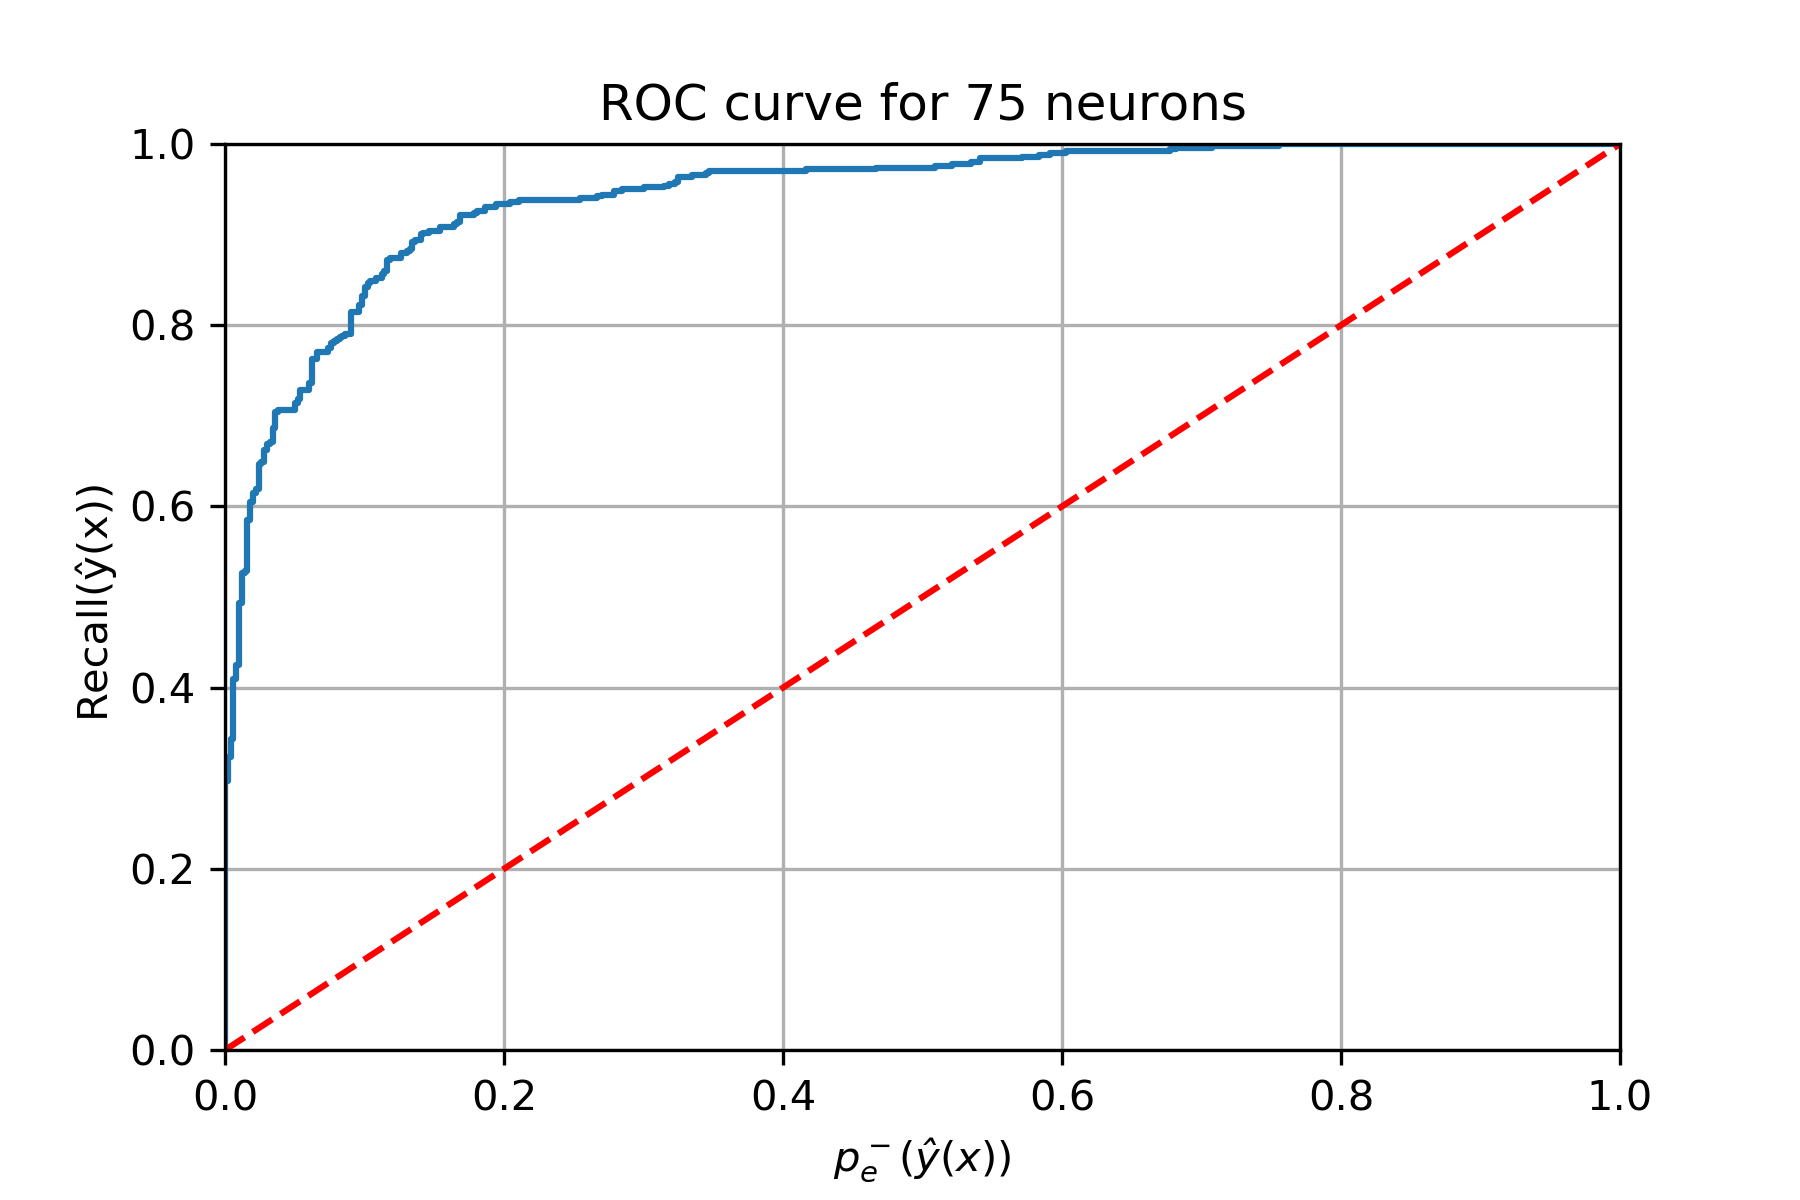
\includegraphics[width=3.85cm]{ROC_75}
        \caption{75 neurons}
        \label{fig:mlp-75_roc}
    \end{subfigure}
    \hfill
    % 100 neurons
    \begin{subfigure}{0.32\textwidth}
        \centering
        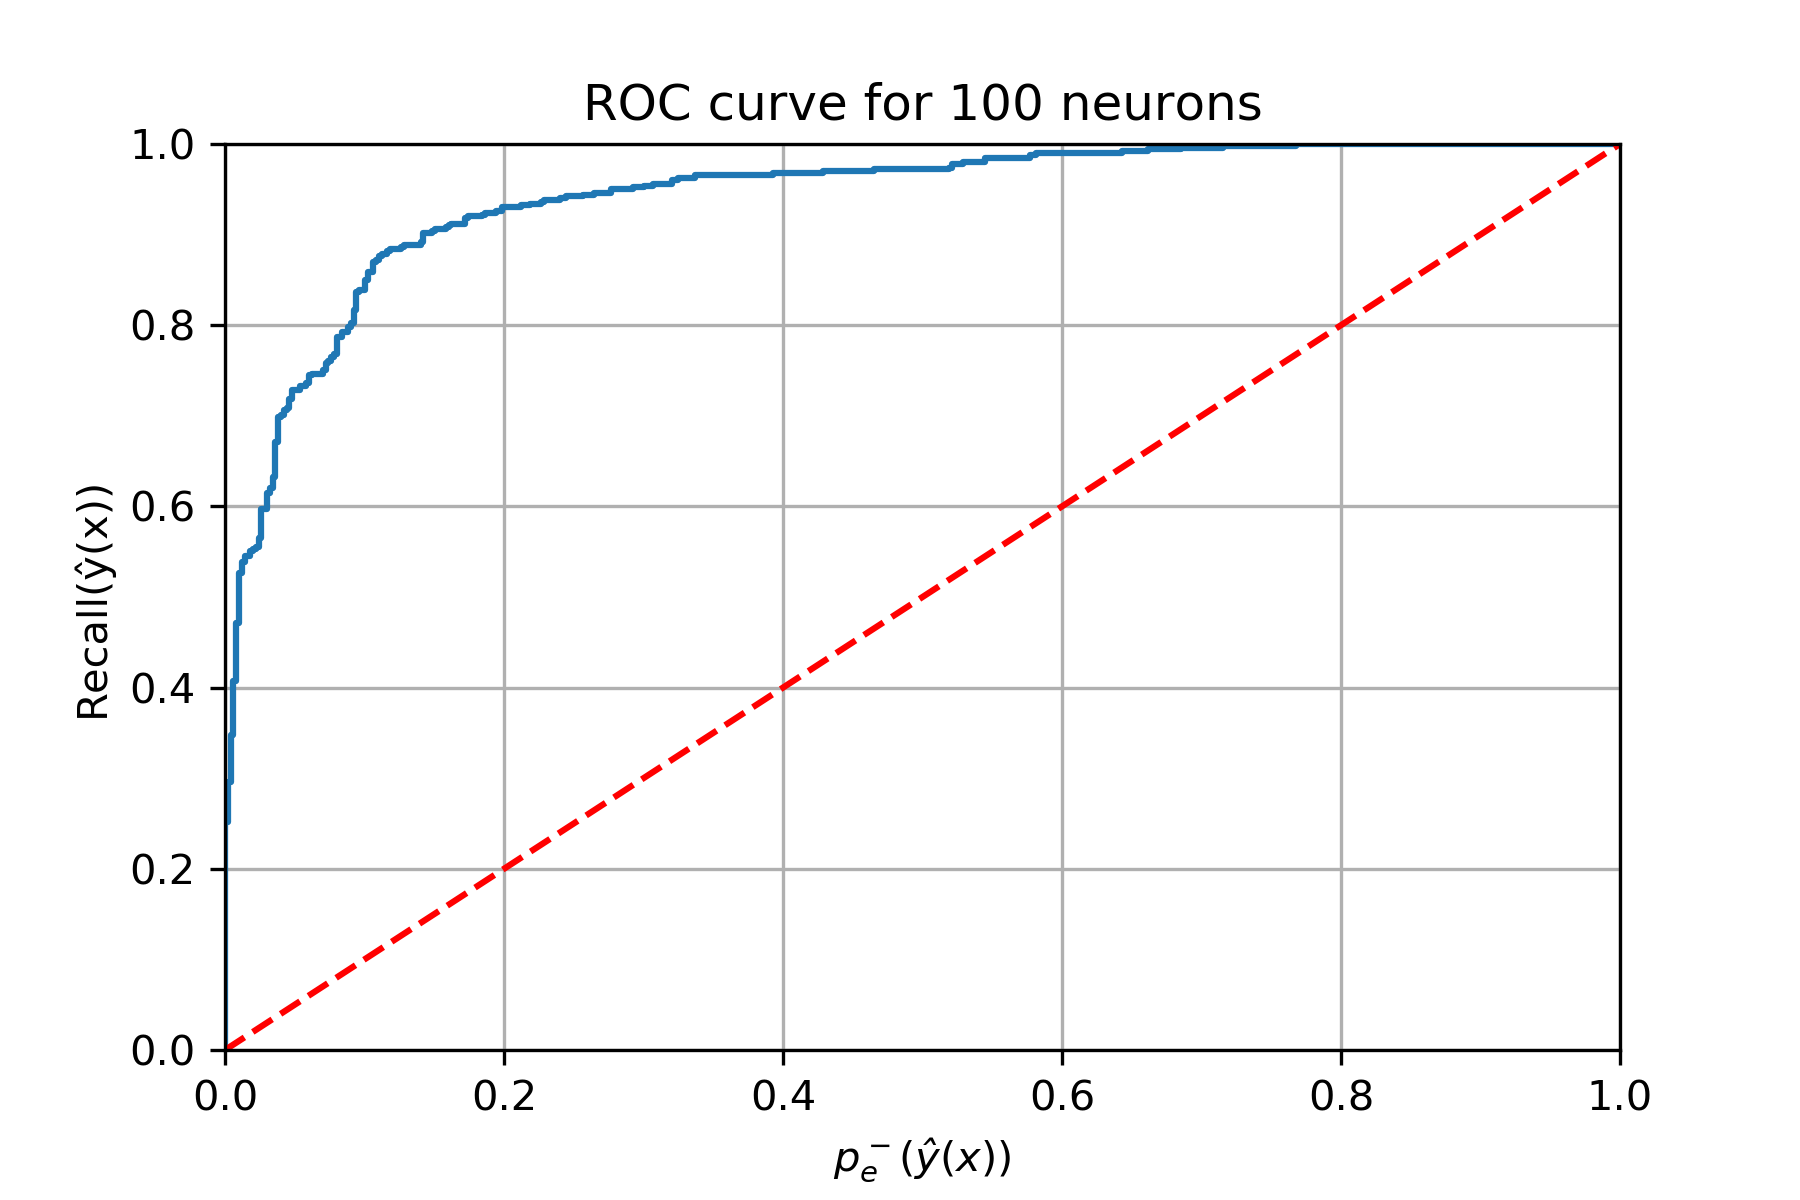
\includegraphics[width=3.85cm]{ROC_100}
        \caption{100 neurons}
        \label{fig:mlp-100_roc}
    \end{subfigure}
    \hfill
    % 300 neurons
    \begin{subfigure}{0.32\textwidth}
        \centering
        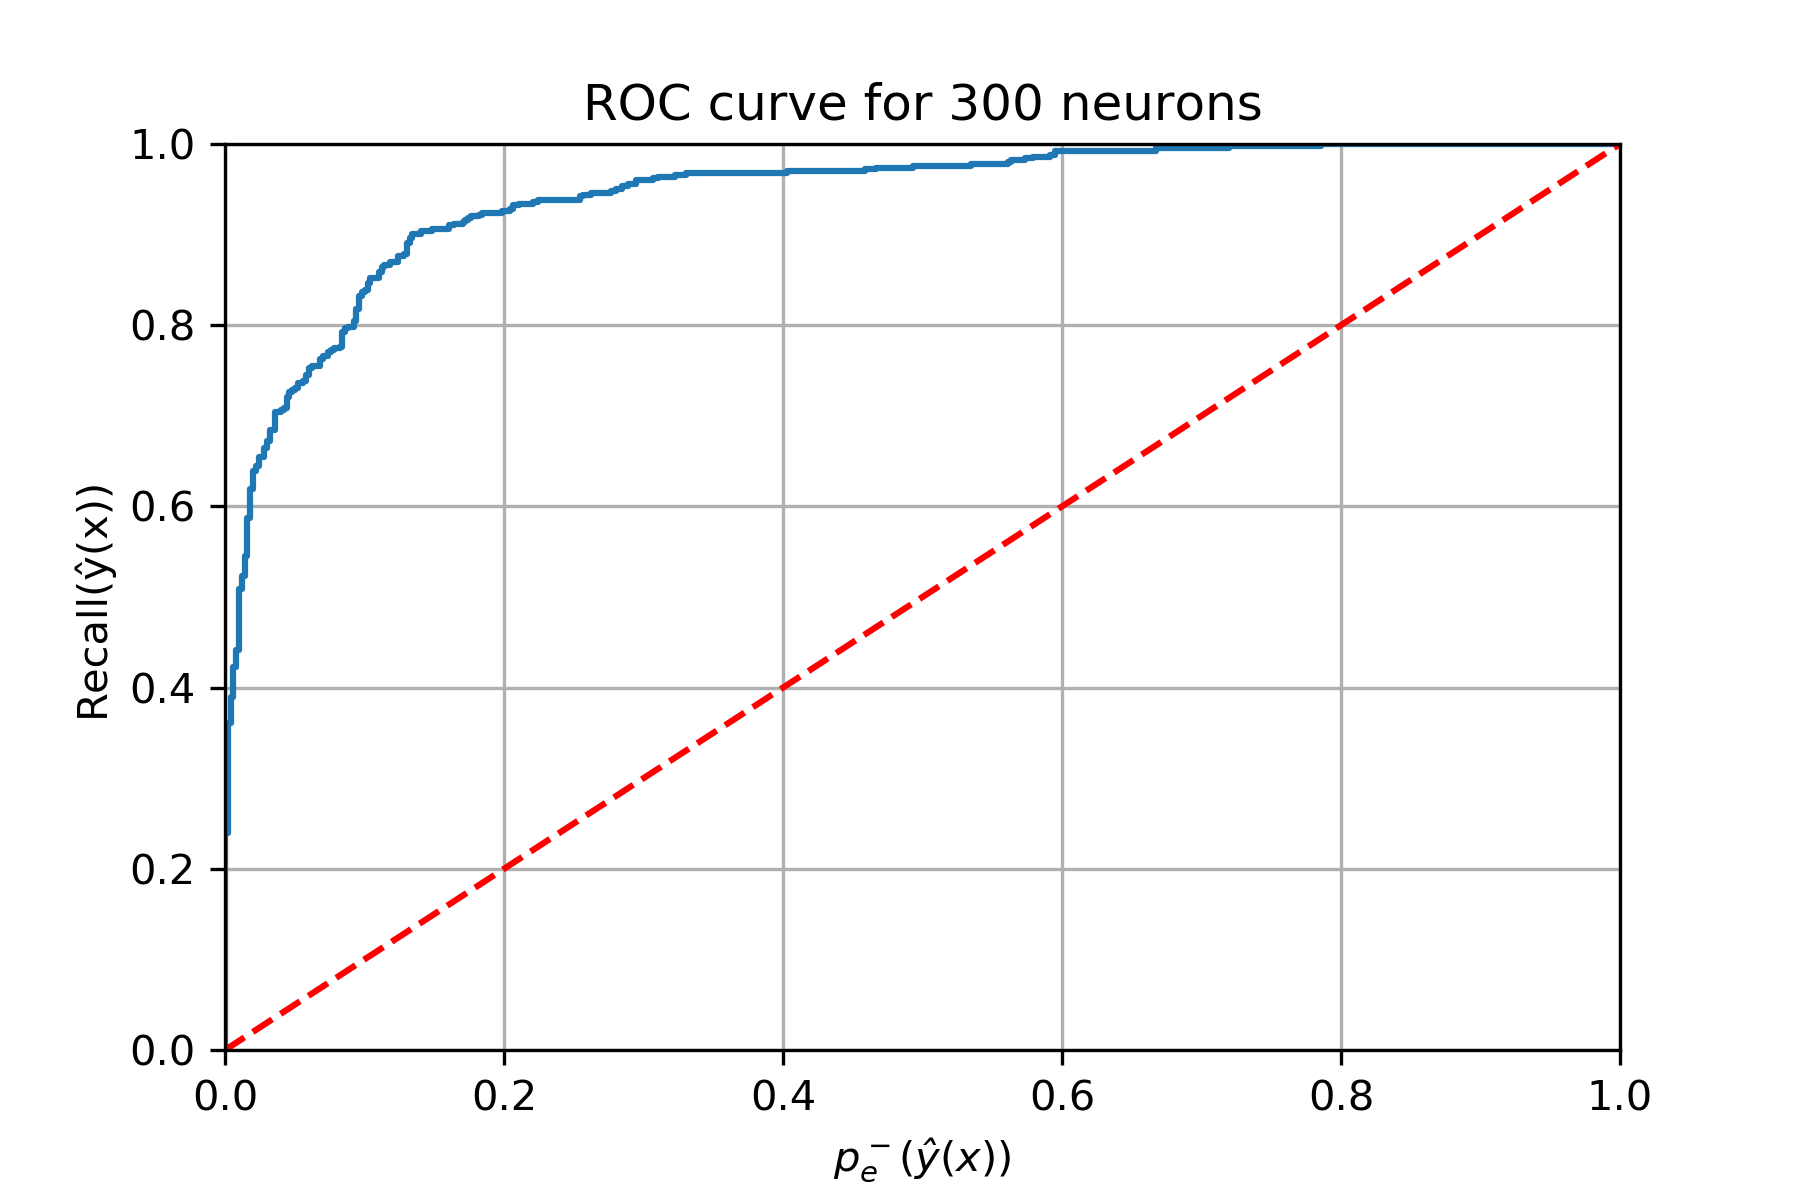
\includegraphics[width=3.85cm]{ROC_300}
        \caption{300 neurons}
        \label{fig:mlp-300_roc}
    \end{subfigure}
    \hfill
    % 1000 neurons
    \begin{subfigure}{0.32\textwidth}
        \centering
        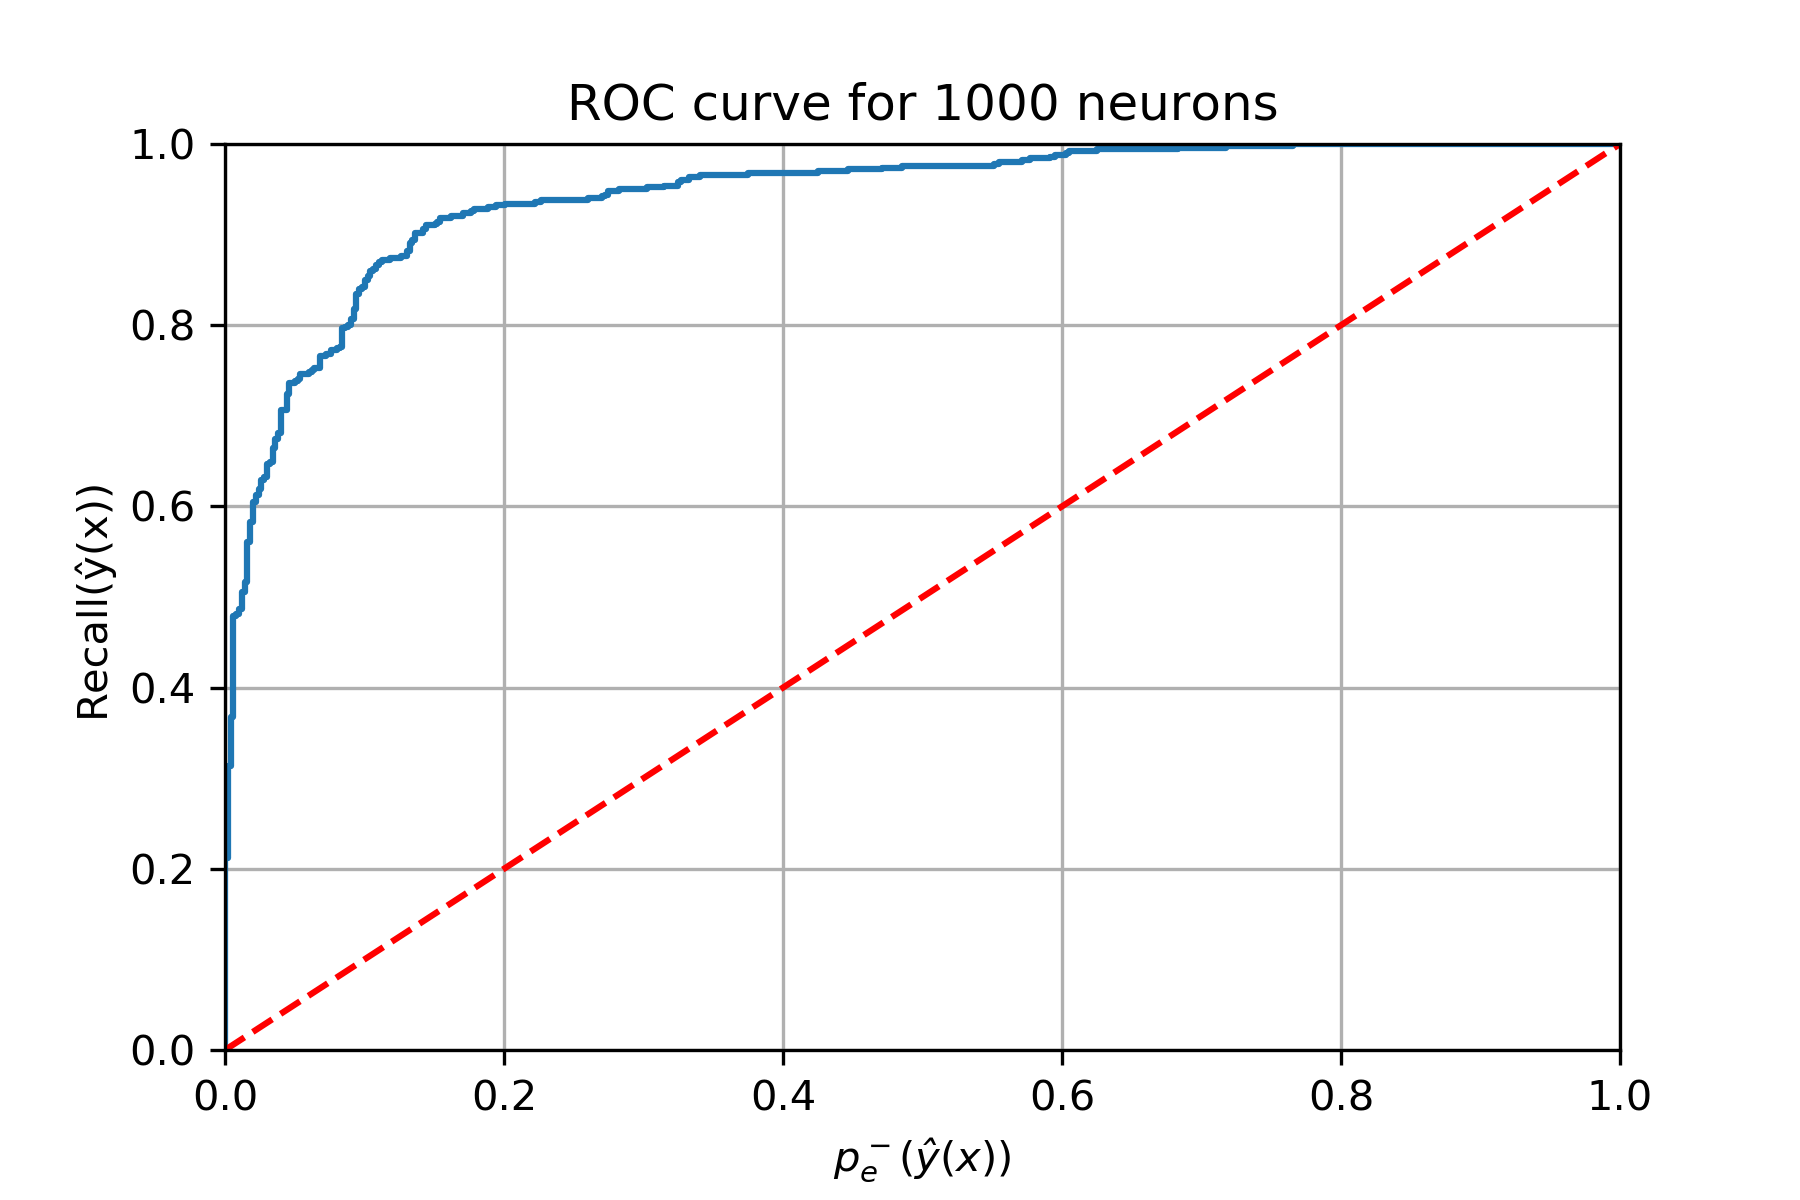
\includegraphics[width=3.85cm]{ROC_1000}
        \caption{1000 neurons}
        \label{fig:mlp-1000_roc}
    \end{subfigure}
    \hfill
    % 5000 neurons
    \begin{subfigure}{0.32\textwidth}
        \centering
        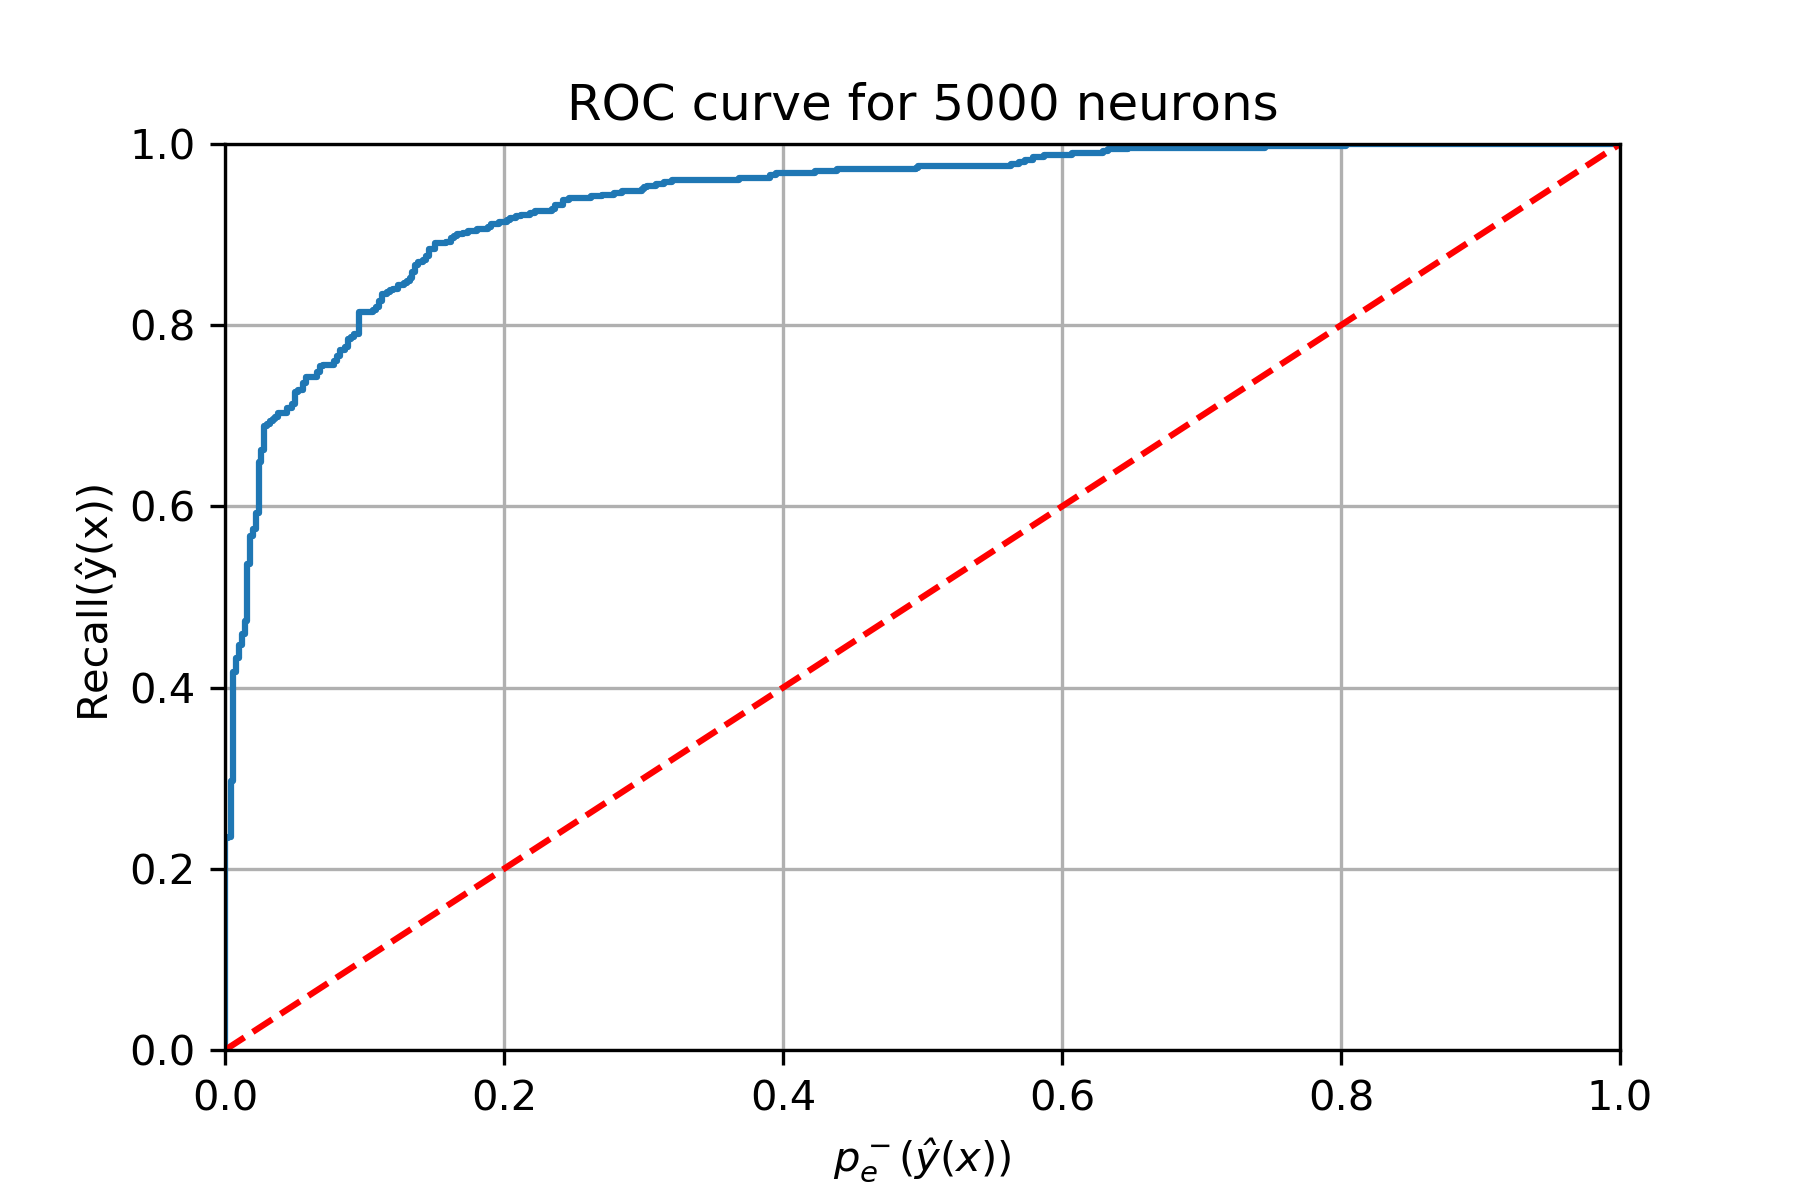
\includegraphics[width=3.85cm]{ROC_5000}
        \caption{5000 neurons}
        \label{fig:mlp-5000_roc}
    \end{subfigure}
    \hfill
    % caption and label
    \caption{ROC curves for MLP with different number of neurons}
    \label{fig:mlp-ROC_N_neurons}
\end{figure}
%-------------------------------------------------

\paragraph{As expected, for networks with few neurons (5 or 25), the model does not have flexibility for separate the classes (underfitting). The opposite is also true, the network with 5000 neurons ``learned'' too much from the dataset compromising the generalization (overfitting). The networks with 75, 100 and 300 neurons presented satisfied results.}

\paragraph{In Figure \ref{fig:mlp-roc_comparasion} we plot all ROC curves under a single plot. This way we can compare the classifiers.}

\begin{figure}[H]
    \centering
    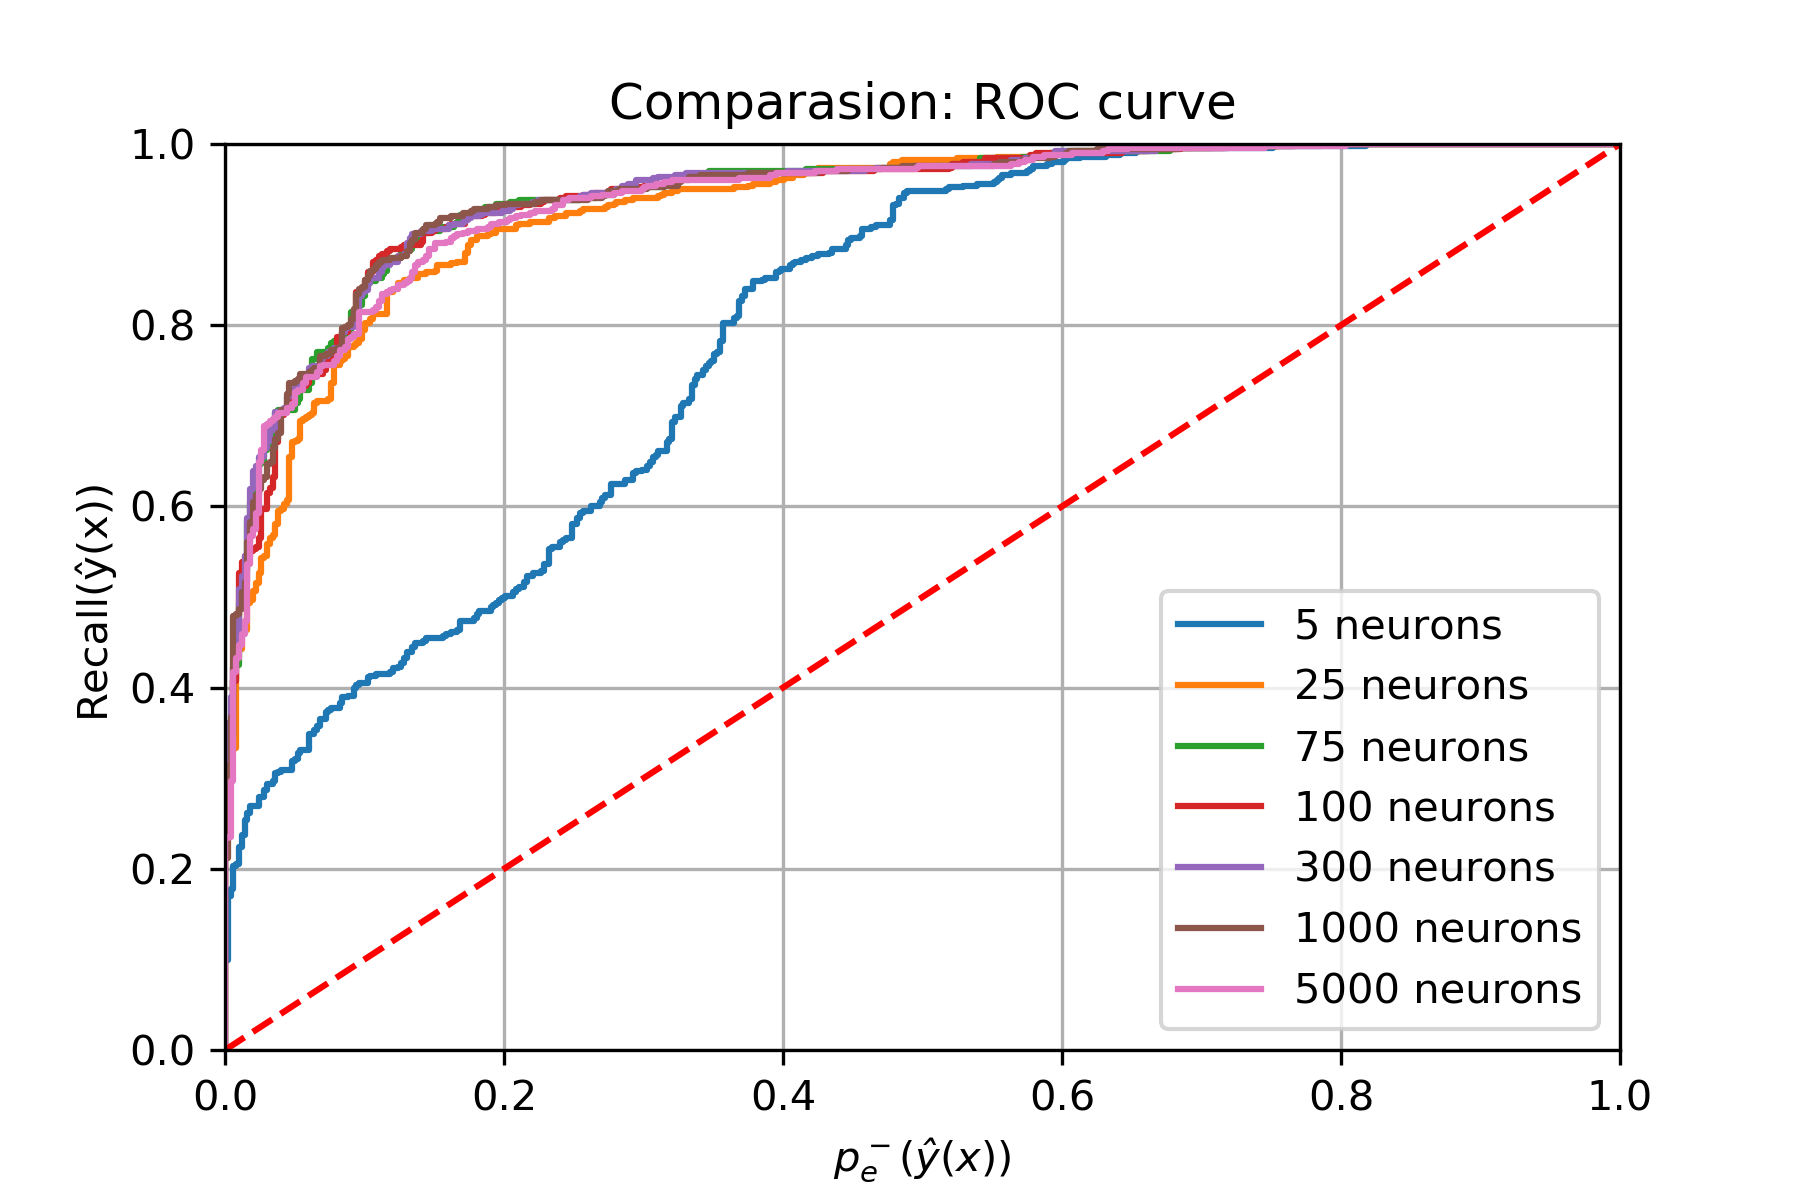
\includegraphics[width=12cm]{ROC_comparasion}
    \caption{Comparison of ROC curves}
    \label{fig:mlp-roc_comparasion}
\end{figure}

\paragraph{We also present in Table \ref{tab:results} other metrics used to evaluate the classifiers. Accuracy in test set, F1-score and area under the ROC curve were calculated. Since the dataset is quite balanced, we are using the simple F1-score, instead of micro and macro.}

\begin{table}[H]
    \begin{center}
        \begin{tabular}{ r|c|c|c|} 
            \cline{2-4}
              & Accuracy & F1-score & ROC area \\
            \cline{2-4}
%            \multirow{2}{4em}{zero-one loss}& cell4 & cell5 & cell6 \\
               5 neurons & 0.733 & 0.762 & 0.7951 \\
              25 neurons & 0.858 & 0.858 & 0.9305 \\
              50 neurons & 0.881 & 0.881 & 0.9477 \\
              75 neurons & 0.870 & 0.868 & 0.9430 \\ 
             100 neurons & 0.870 & 0.866 & 0.9415 \\
             300 neurons & 0.872 & 0.870 & 0.9434 \\
            1000 neurons & 0.877 & 0.875 & 0.9427 \\
            5000 neurons & 0.860 & 0.858 & 0.9376 \\
            \cline{2-4}
        \end{tabular}
    \end{center}
    \caption{Comparison of results between networks with different number of neurons}
    \label{tab:results}
\end{table}

\newpage
%=================================================
\subsection{Support Vector Machine (SVM)}
%=================================================

%--------------------------------------
\subsubsection{e) SVM decision regions and support vectors}
%--------------------------------------

\paragraph{We now developed a SVM to do the classification. To find the hyperparameter C we used cross-validation sweeping C from 0.1 until 10 in steps of 0.1. The C for minimum error in validation set found was 8.3. The Figure \ref{fig:svm-decision_regions} shows the decision regions for this value of C plotted with the same function used in the MLP. In Figure \ref{fig:svm-support_vectors} we can see the support vectors identified.}

\begin{figure}[H]
    \centering
    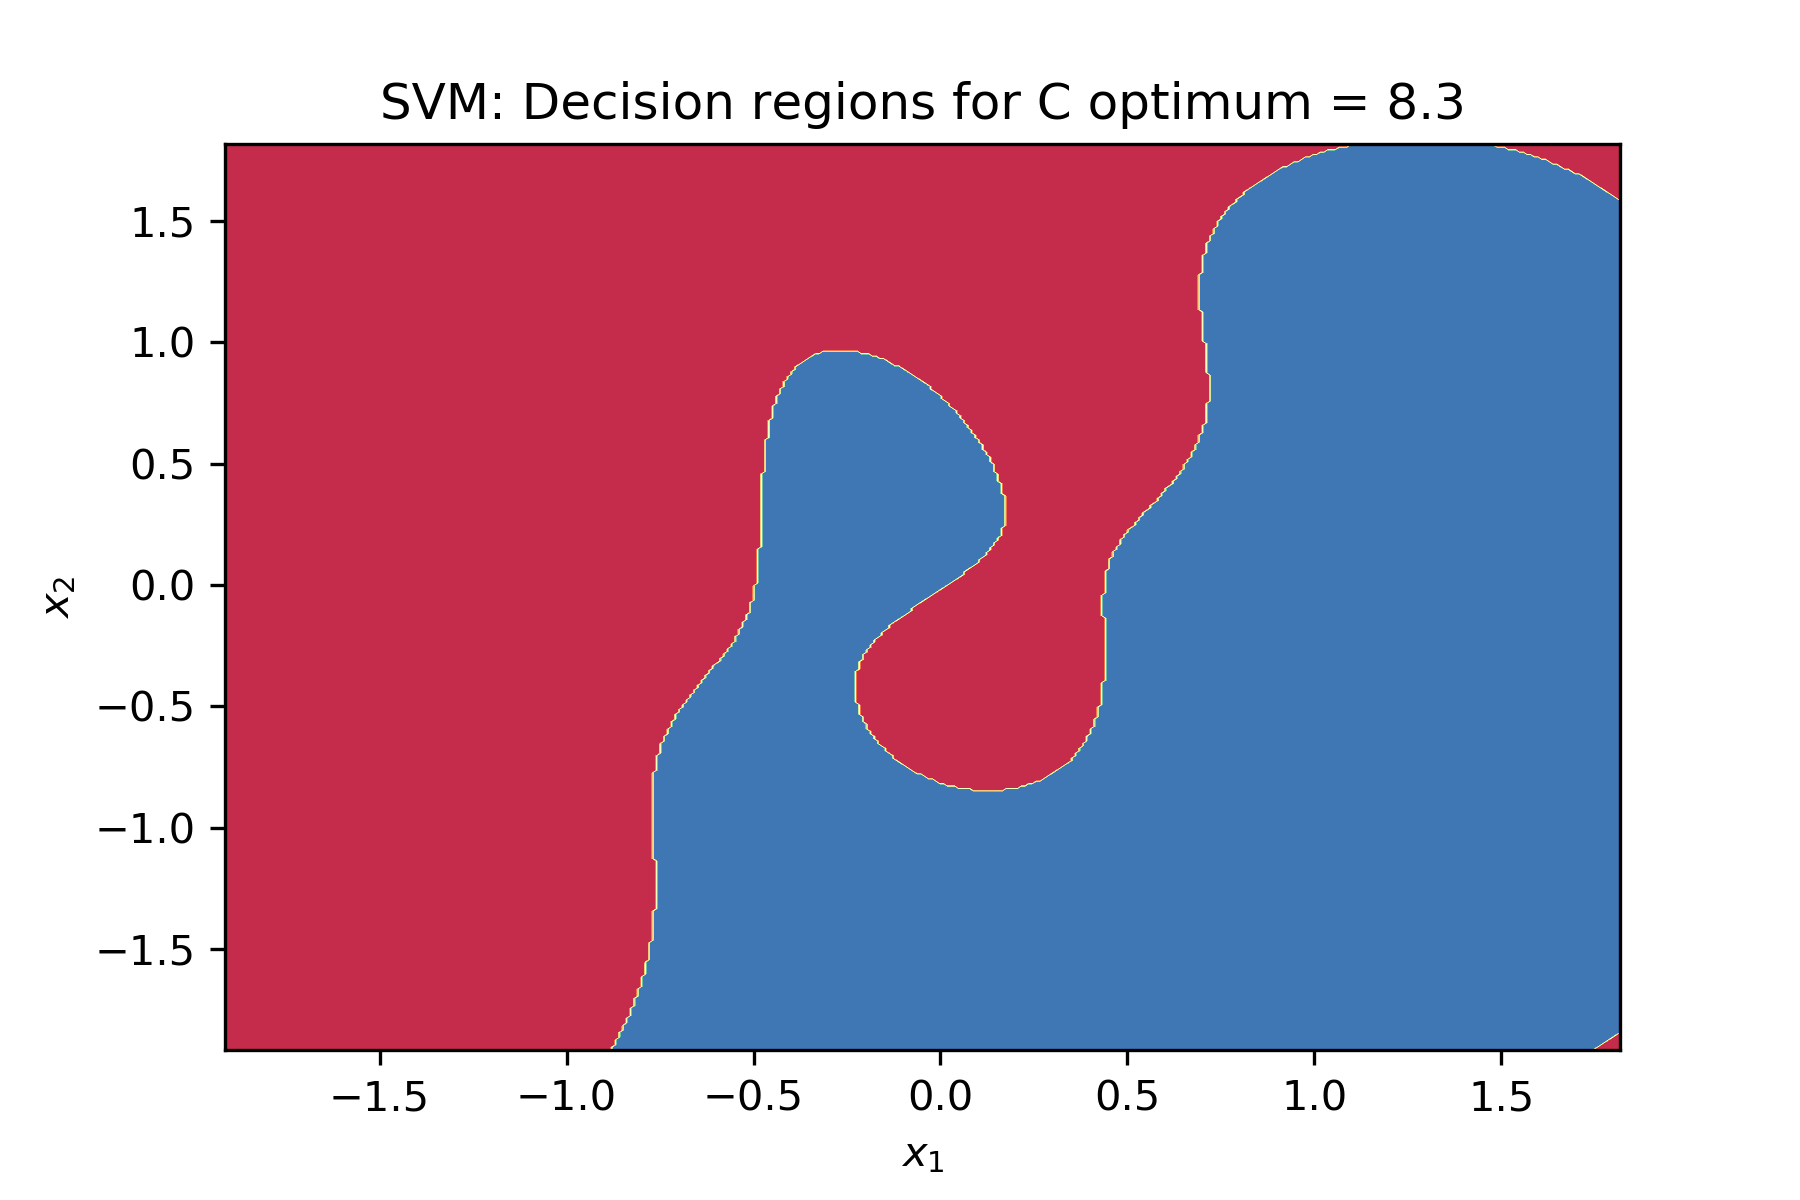
\includegraphics[width=12cm]{svm_decision_region}
    \caption{Decision regions}
    \label{fig:svm-decision_regions}
\end{figure}

\begin{figure}[H]
    \centering
    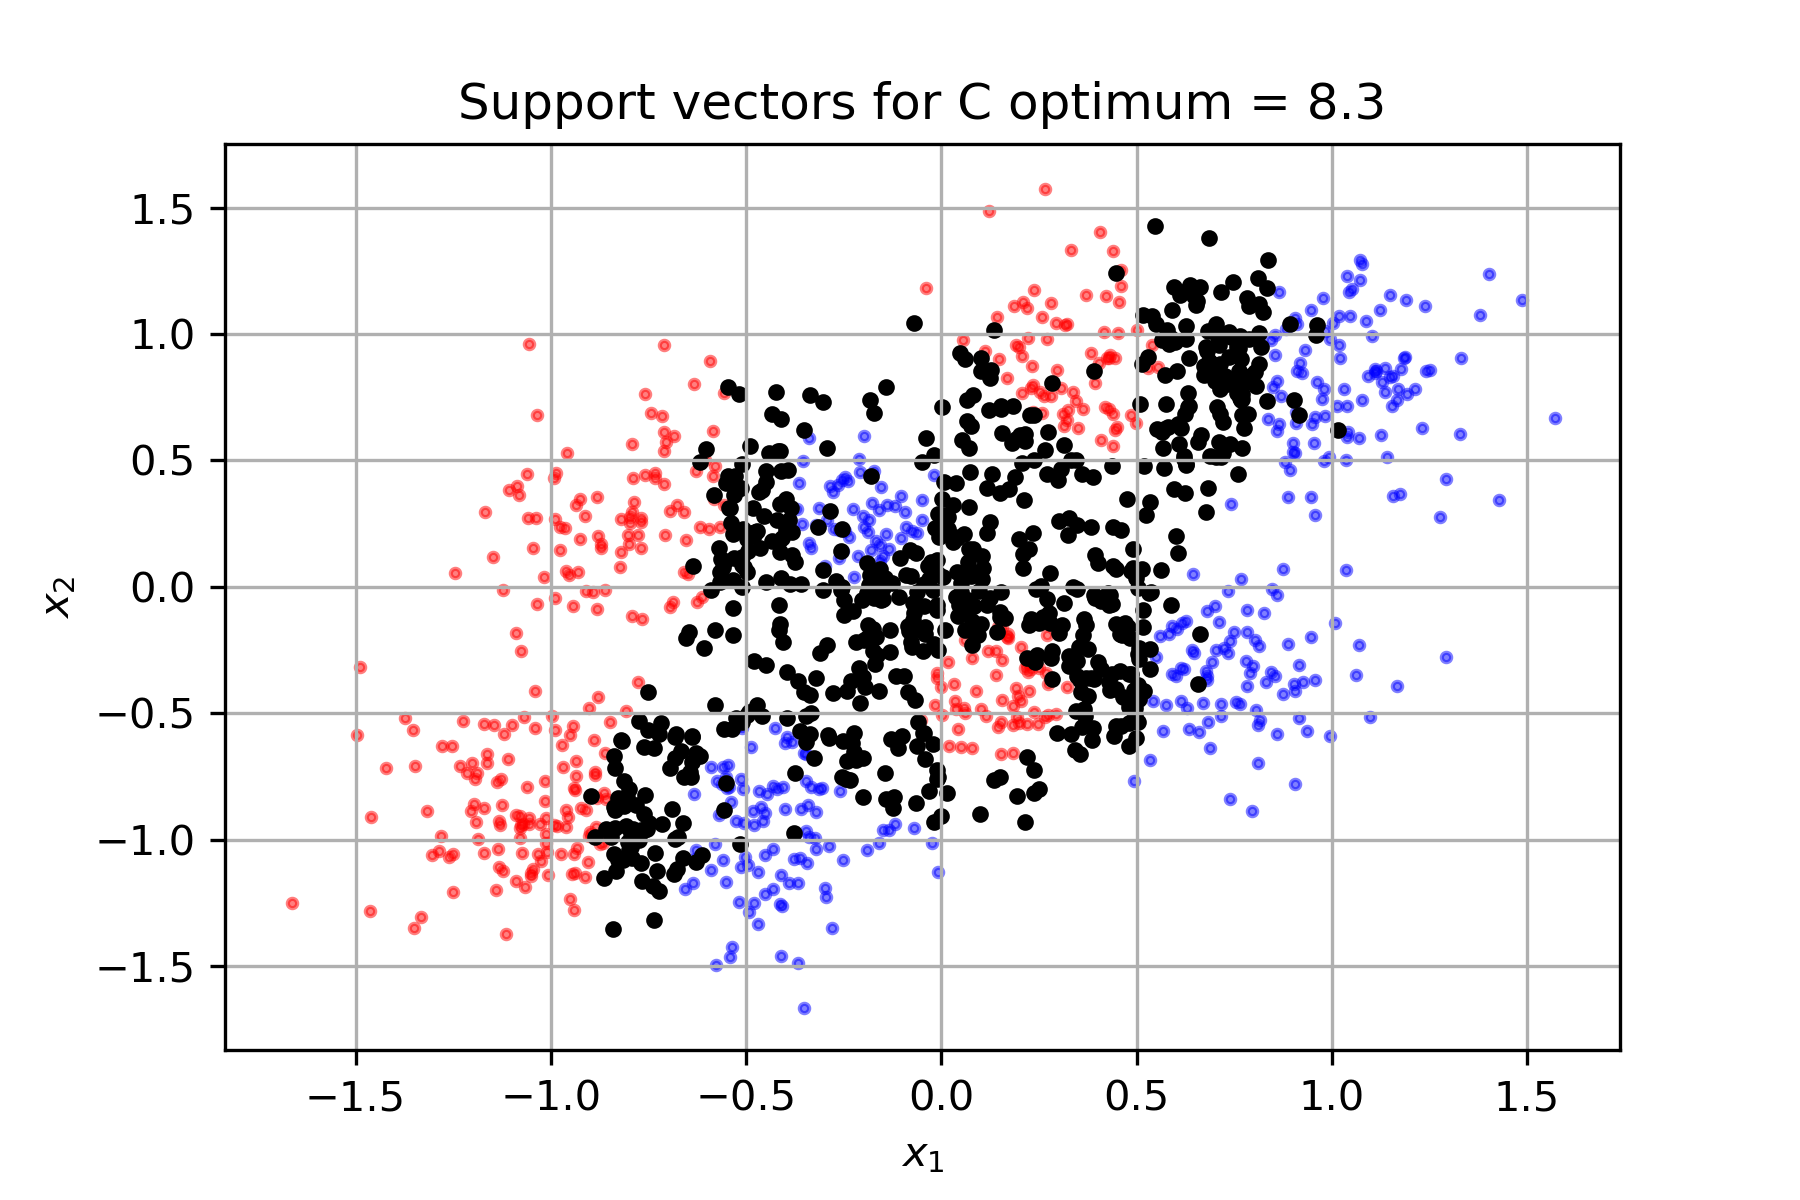
\includegraphics[width=12cm]{support_vectors}
    \caption{Support vectors}
    \label{fig:svm-support_vectors}
\end{figure}

%--------------------------------------
\subsubsection{f) Applying SVM model to test set}
%--------------------------------------

\paragraph{We then used the model along with the test set. Figure \ref{fig:svm-test_set_output} shows the output generated for each data. The accuracy obtained was 0.877, indicating an error of 12.3\%.}

\begin{figure}[H]
    \centering
    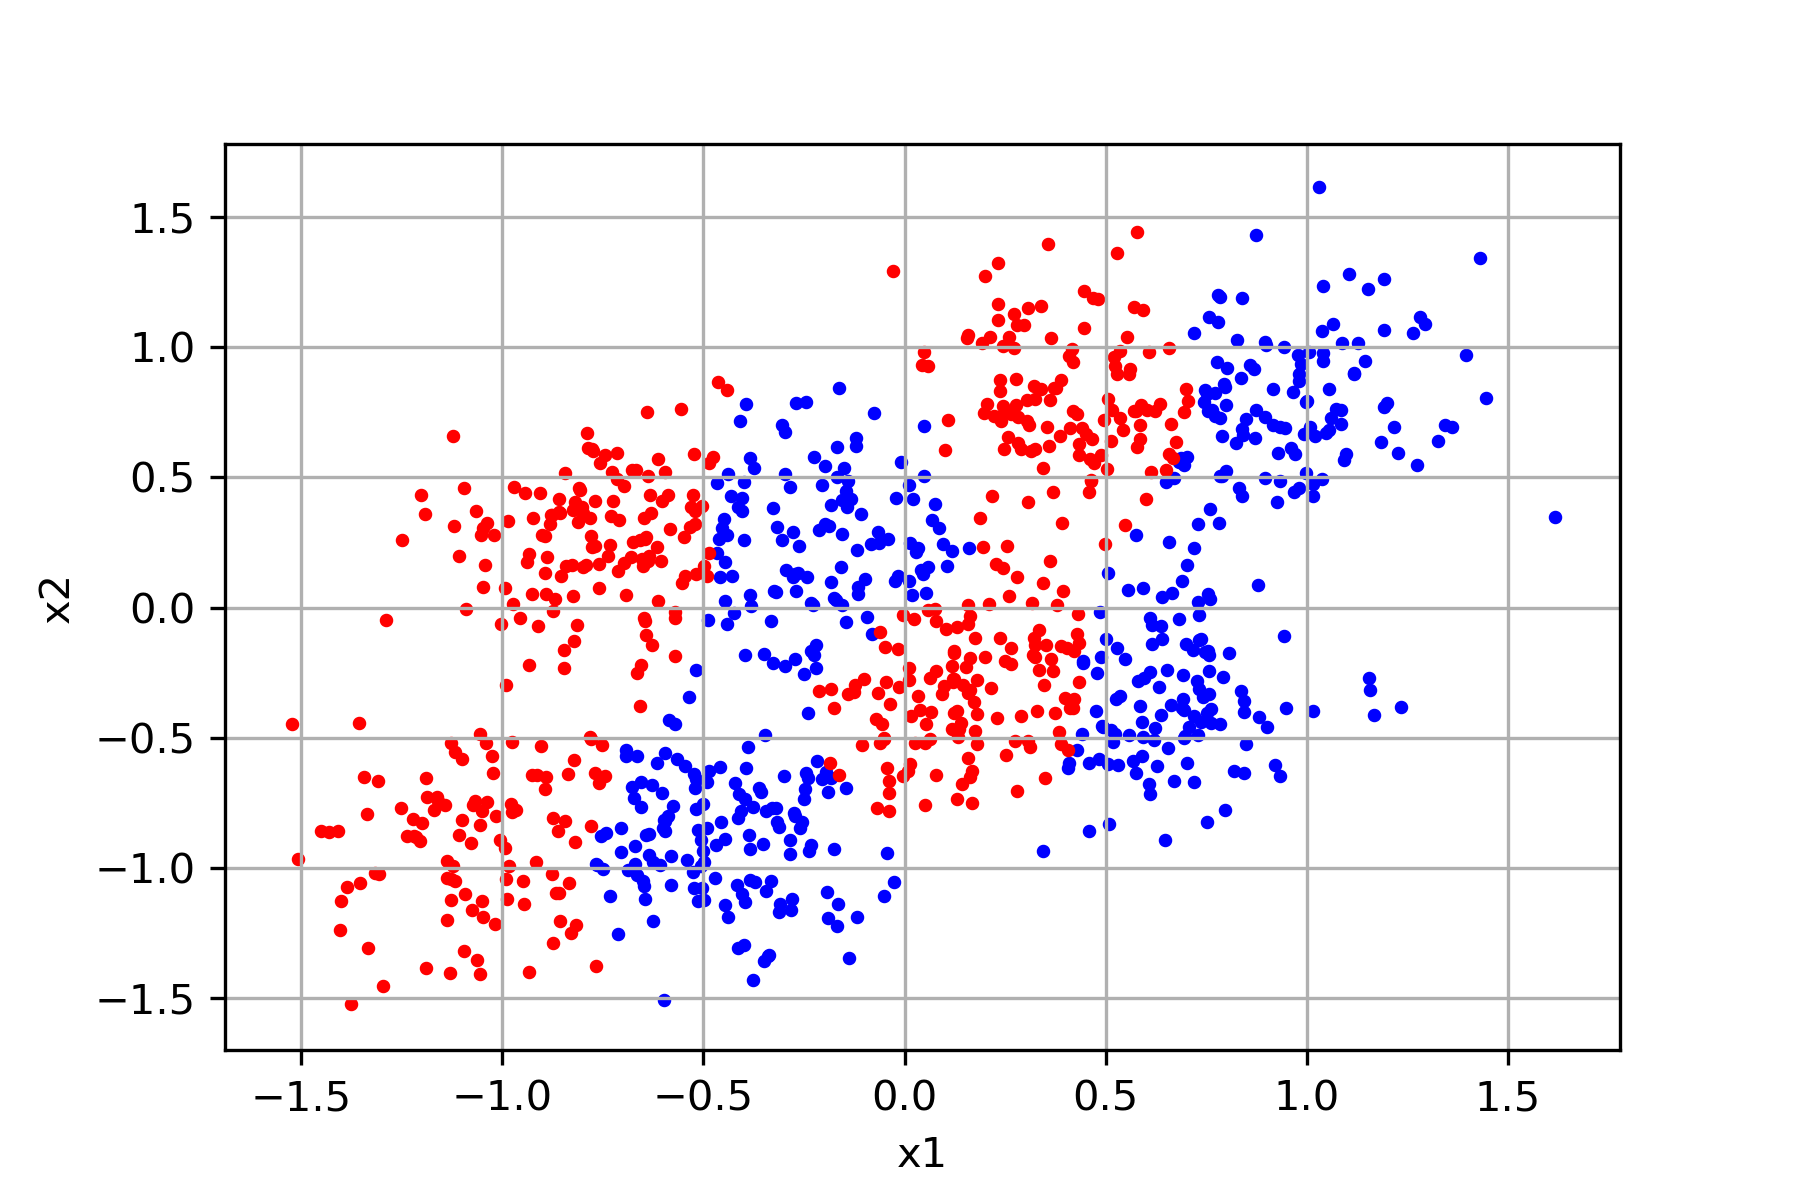
\includegraphics[width=12cm]{svm_test_set_output}
    \caption{SVM predicted output for test set}
    \label{fig:svm-test_set_output}
\end{figure}

%--------------------------------------
\subsubsection{g) Experimenting different kernel parameters and values of C}
%--------------------------------------

\paragraph{We now used different values of the hyperparameter C to see what impact this would cause in the classifier. In Figure \ref{fig:svm-decision_regions_support_vectos_C} we can see the decision regions and the respective support vectors for values of C equal to 0.1, 1, 20 and 1000.}

%-------------------------------------------------
%\newpage
% decision regions for different values of hyperparameter C
% and the respective support vectors

\begin{figure}[H]
    %-----------------------------------
    \centering
    % decision regions (C = 0.1)
    \begin{subfigure}{0.45\textwidth}
        \centering
        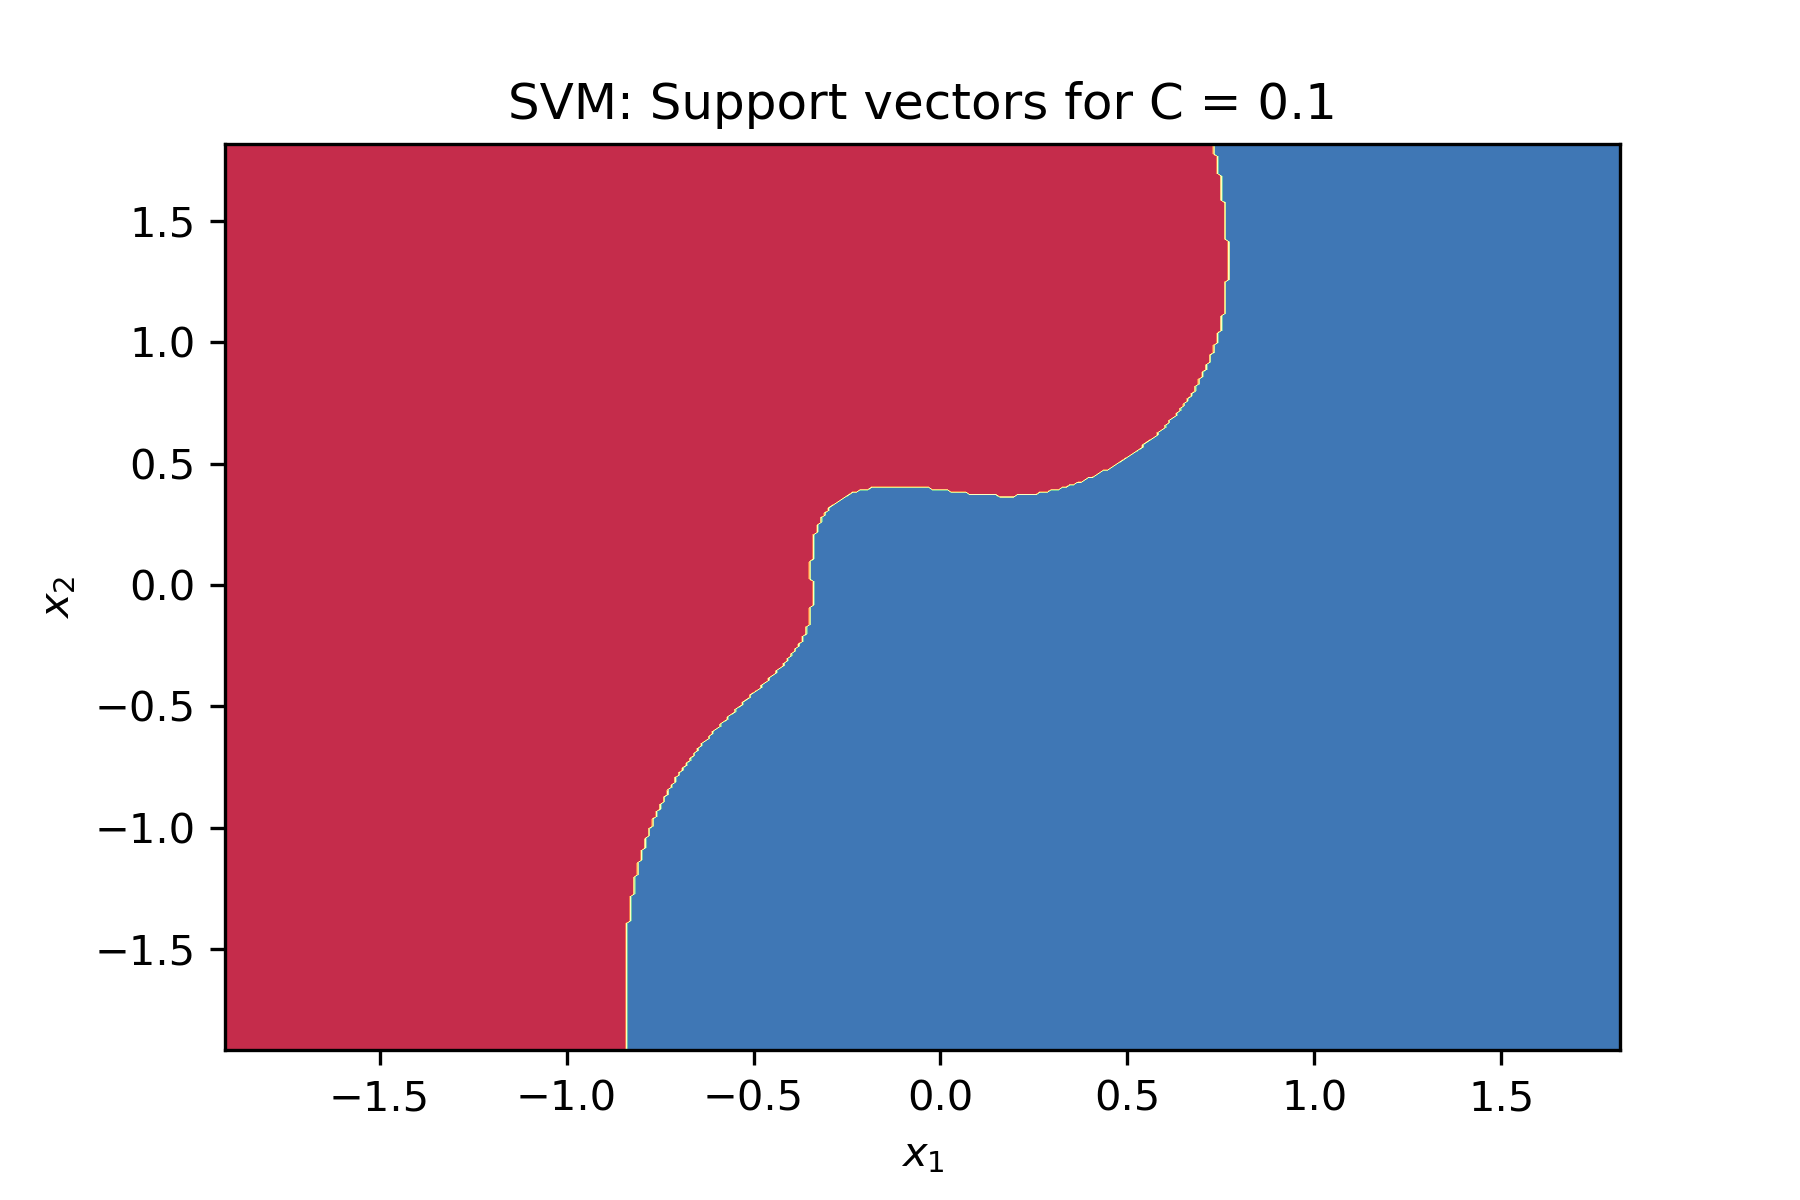
\includegraphics[width=7cm]{decision_region_C_0d1}
        \caption{Decision regions for C = 0.1}
        \label{fig:svm-decision_region_C_0d1}
    \end{subfigure}
    \hfill
    % support vectors (C = 0.1)
    \begin{subfigure}{0.45\textwidth}
        \centering
        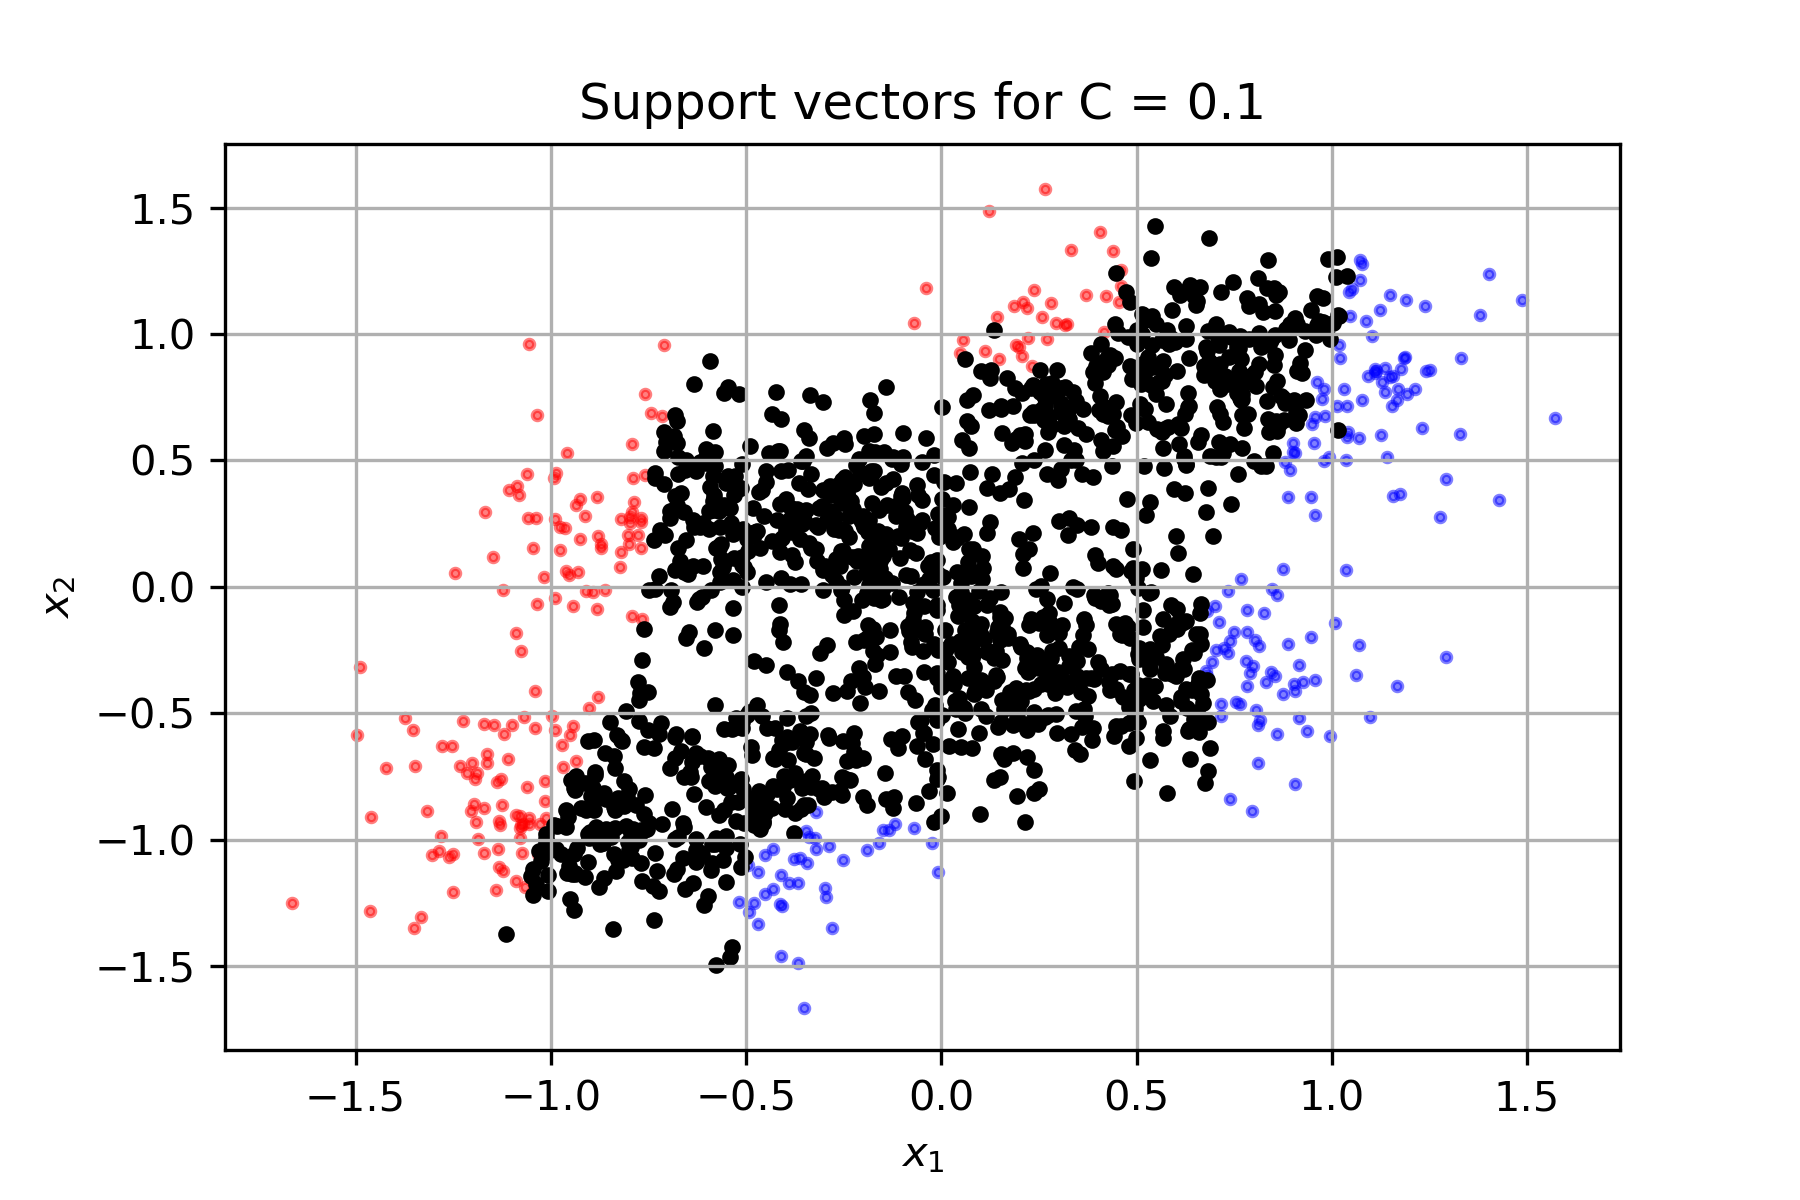
\includegraphics[width=7cm]{support_vectors_C_0d1}
        \caption{Support vectors for C = 0.1}
        \label{fig:svm-support_vectors_C_0d1}
    \end{subfigure}
    %-----------------------------------
    % decision regions (C = 1.0)
    \begin{subfigure}{0.45\textwidth}
        \centering
        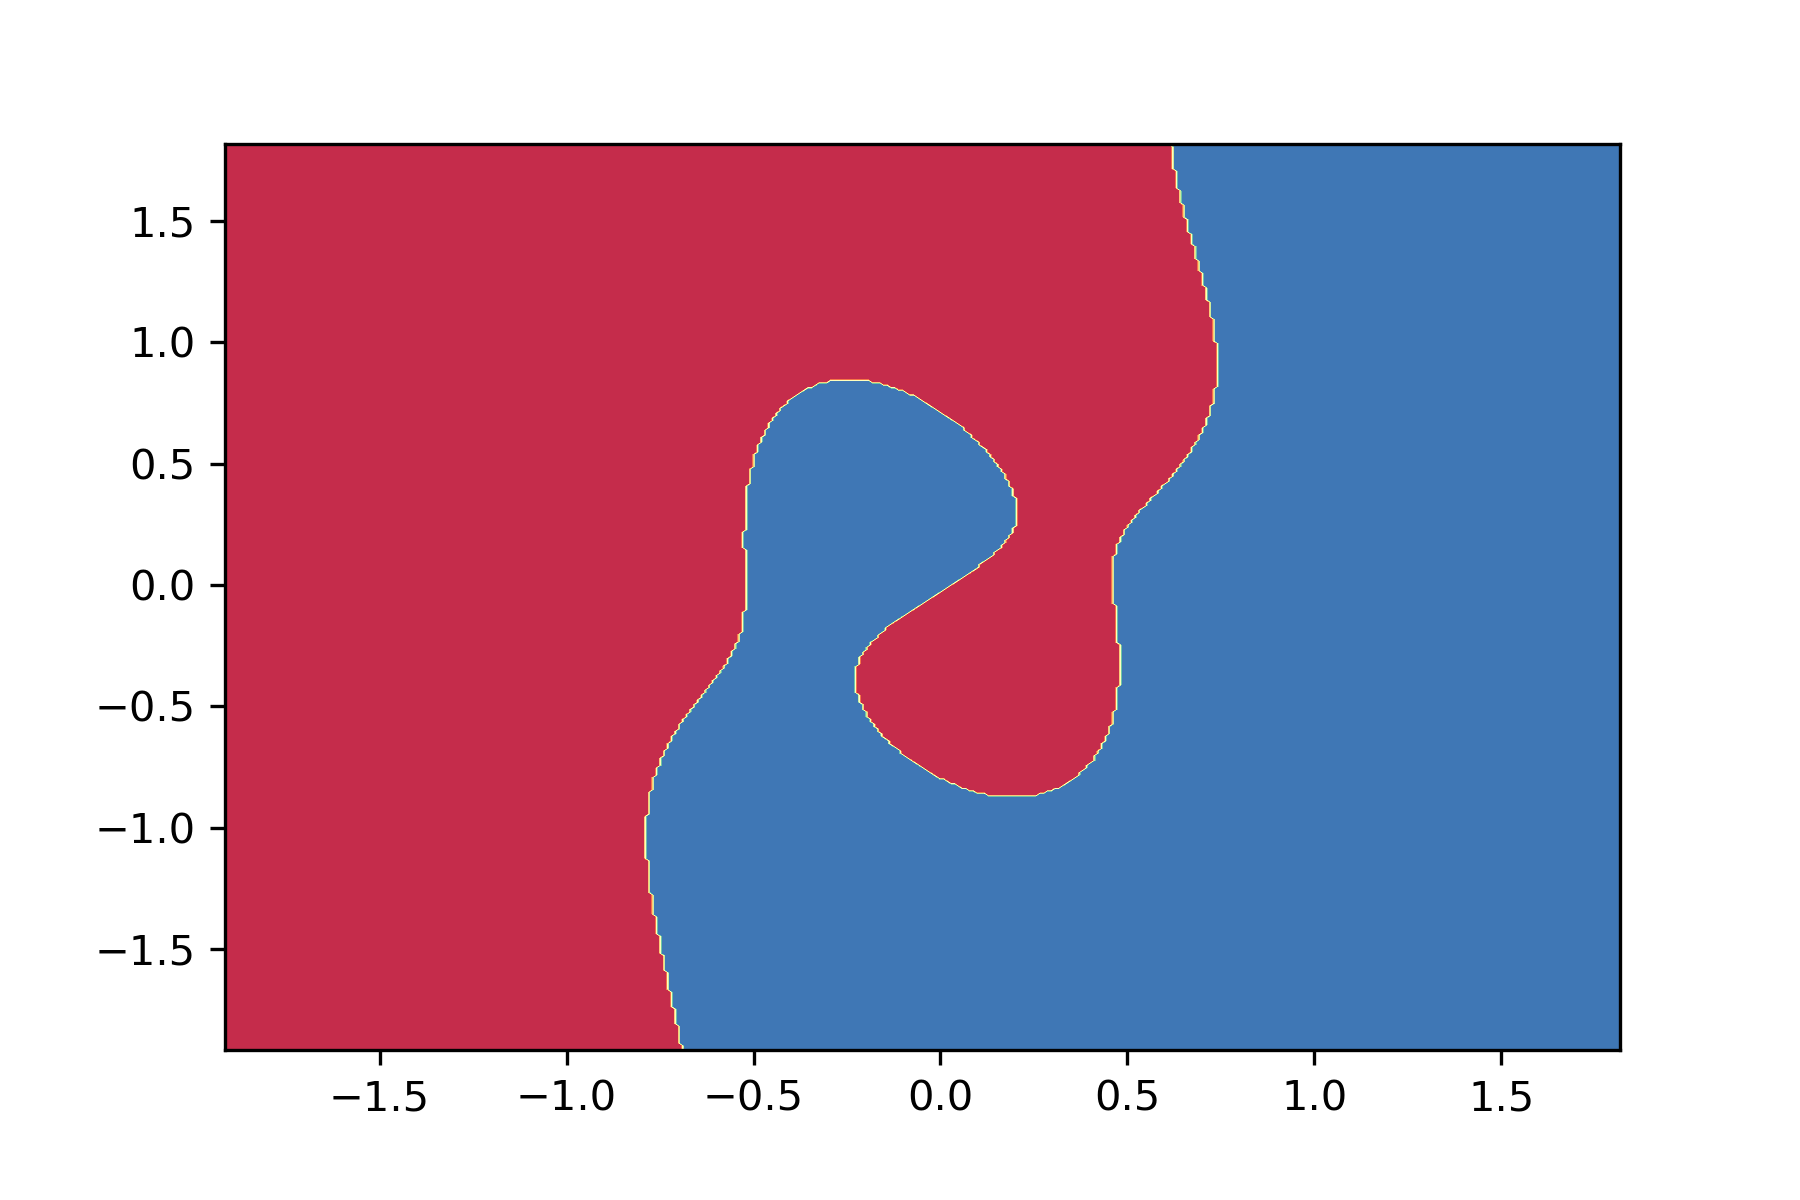
\includegraphics[width=7cm]{decision_region_C_1}
        \caption{Decision regions for C = 1.0}
        \label{fig:svm-decision_region_C_1}
    \end{subfigure}
    \hfill
    % support vectors (C = 1.0)
    \begin{subfigure}{0.45\textwidth}
        \centering
        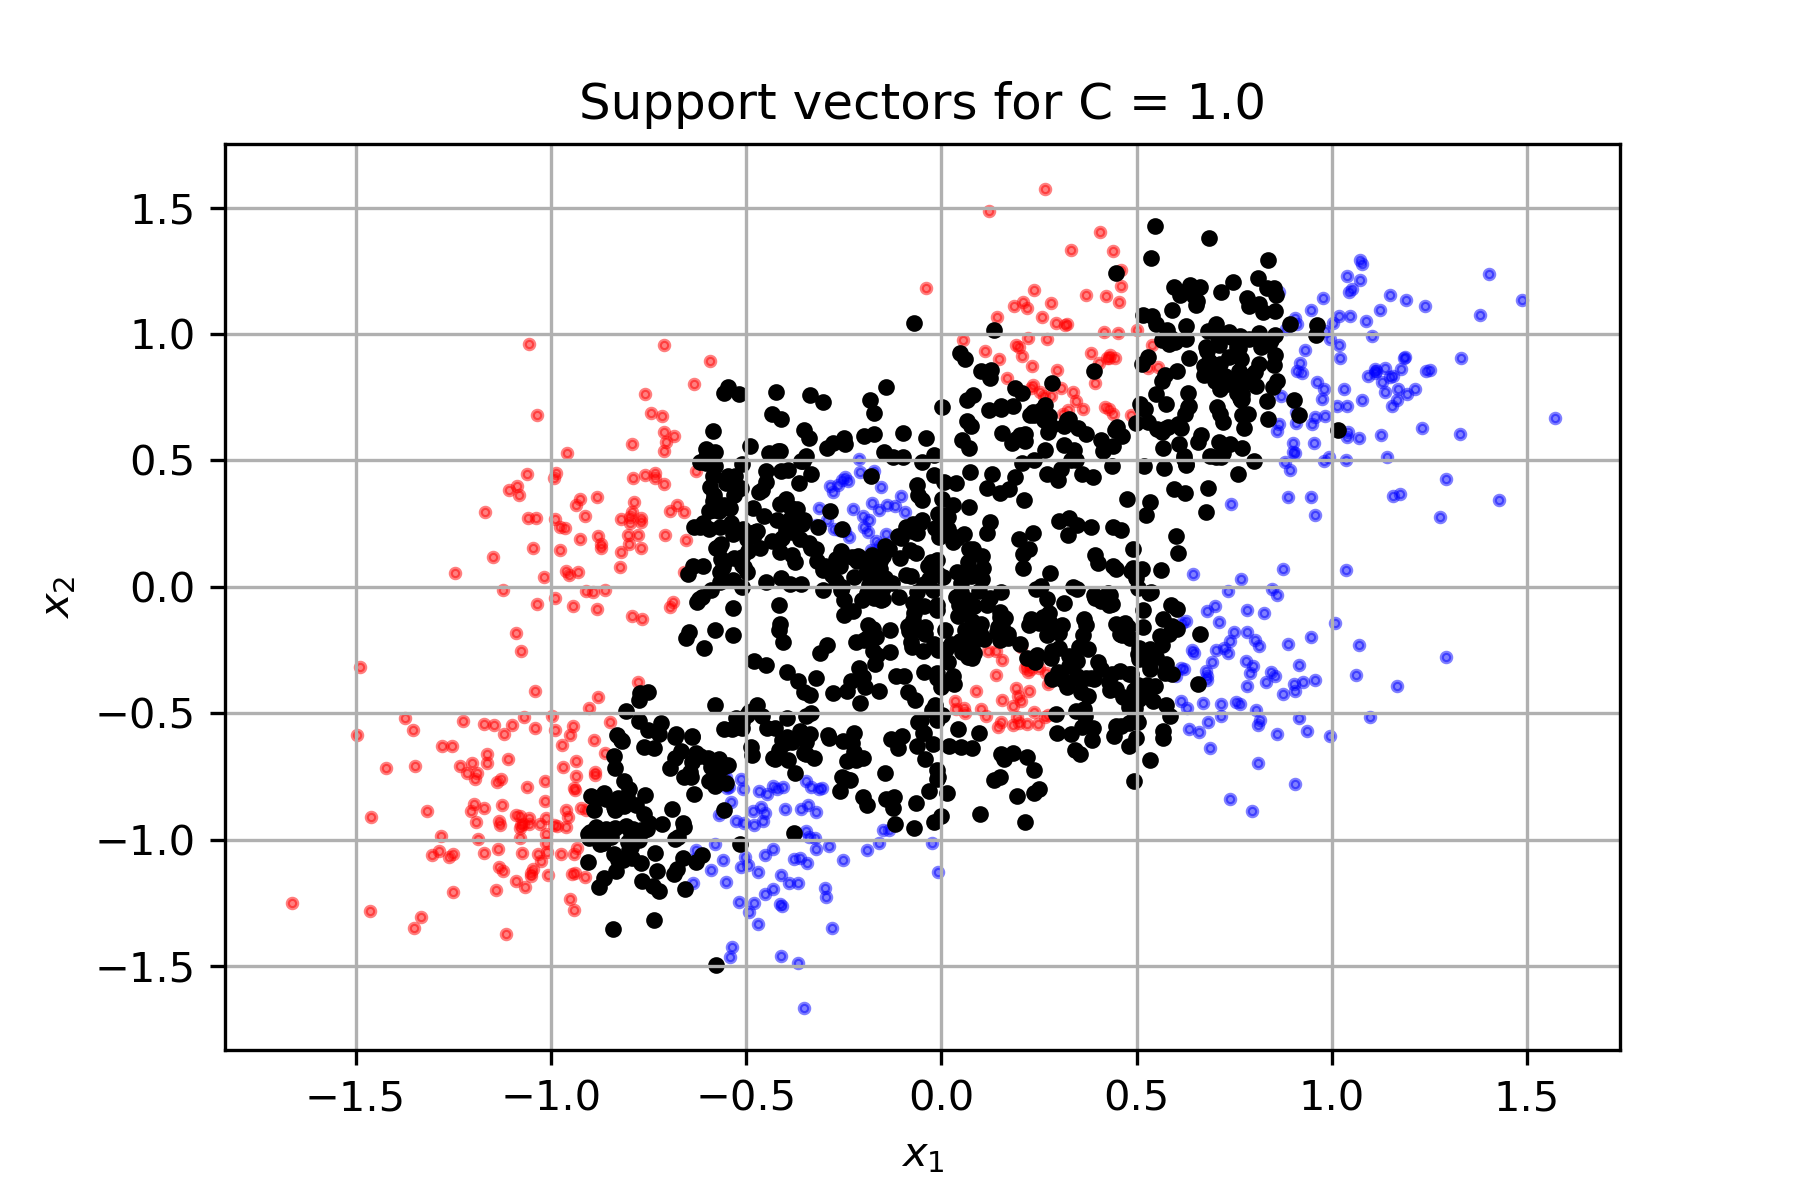
\includegraphics[width=7cm]{support_vectors_C_1}
        \caption{Support vectors for C = 1.0}
        \label{fig:svm-support_vectors_C_1}
    \end{subfigure}
    %-----------------------------------
    % decision regions (C = 20)
    \begin{subfigure}{0.45\textwidth}
        \centering
        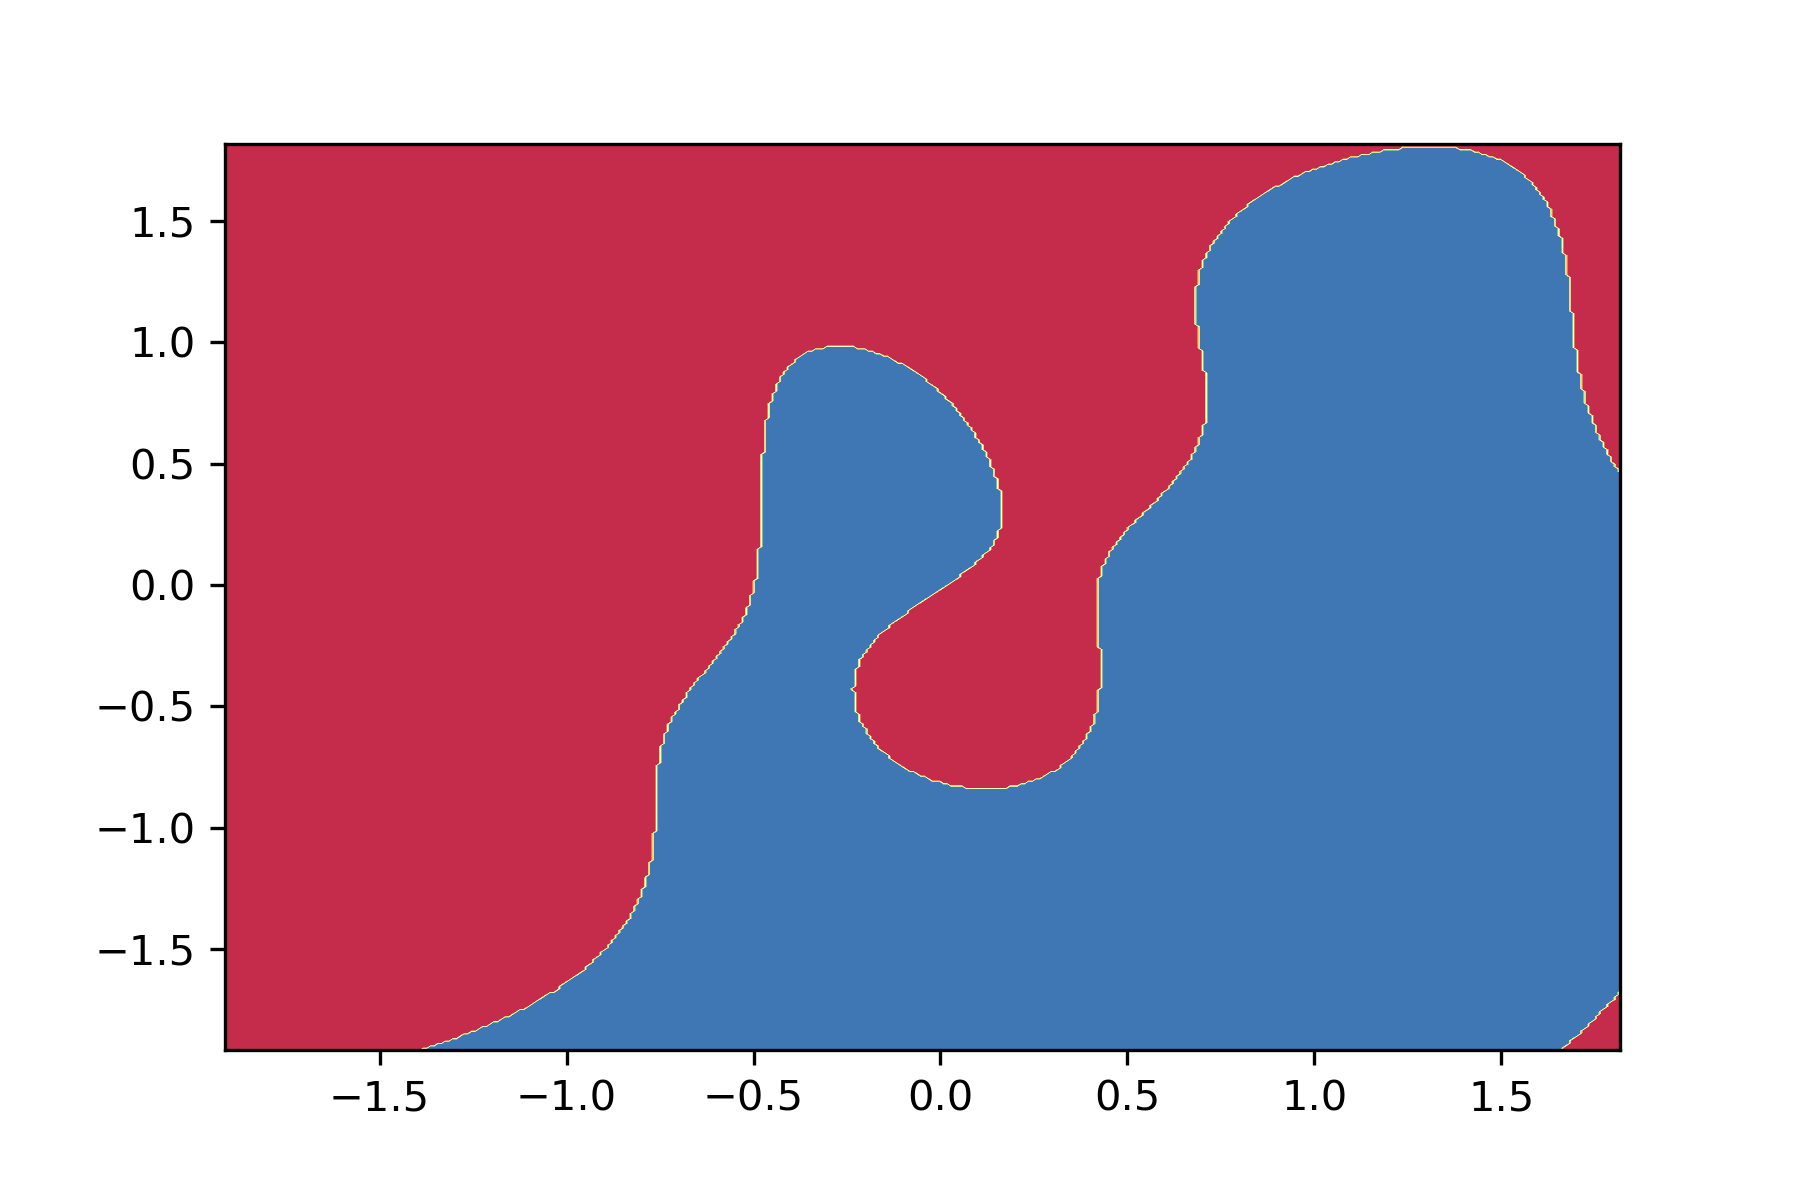
\includegraphics[width=7cm]{decision_region_C_20}
        \caption{Decision regions for C = 20}
        \label{fig:svm-decision_region_C_20}
    \end{subfigure}
    \hfill
    % support vectors (C = 20)
    \begin{subfigure}{0.45\textwidth}
        \centering
        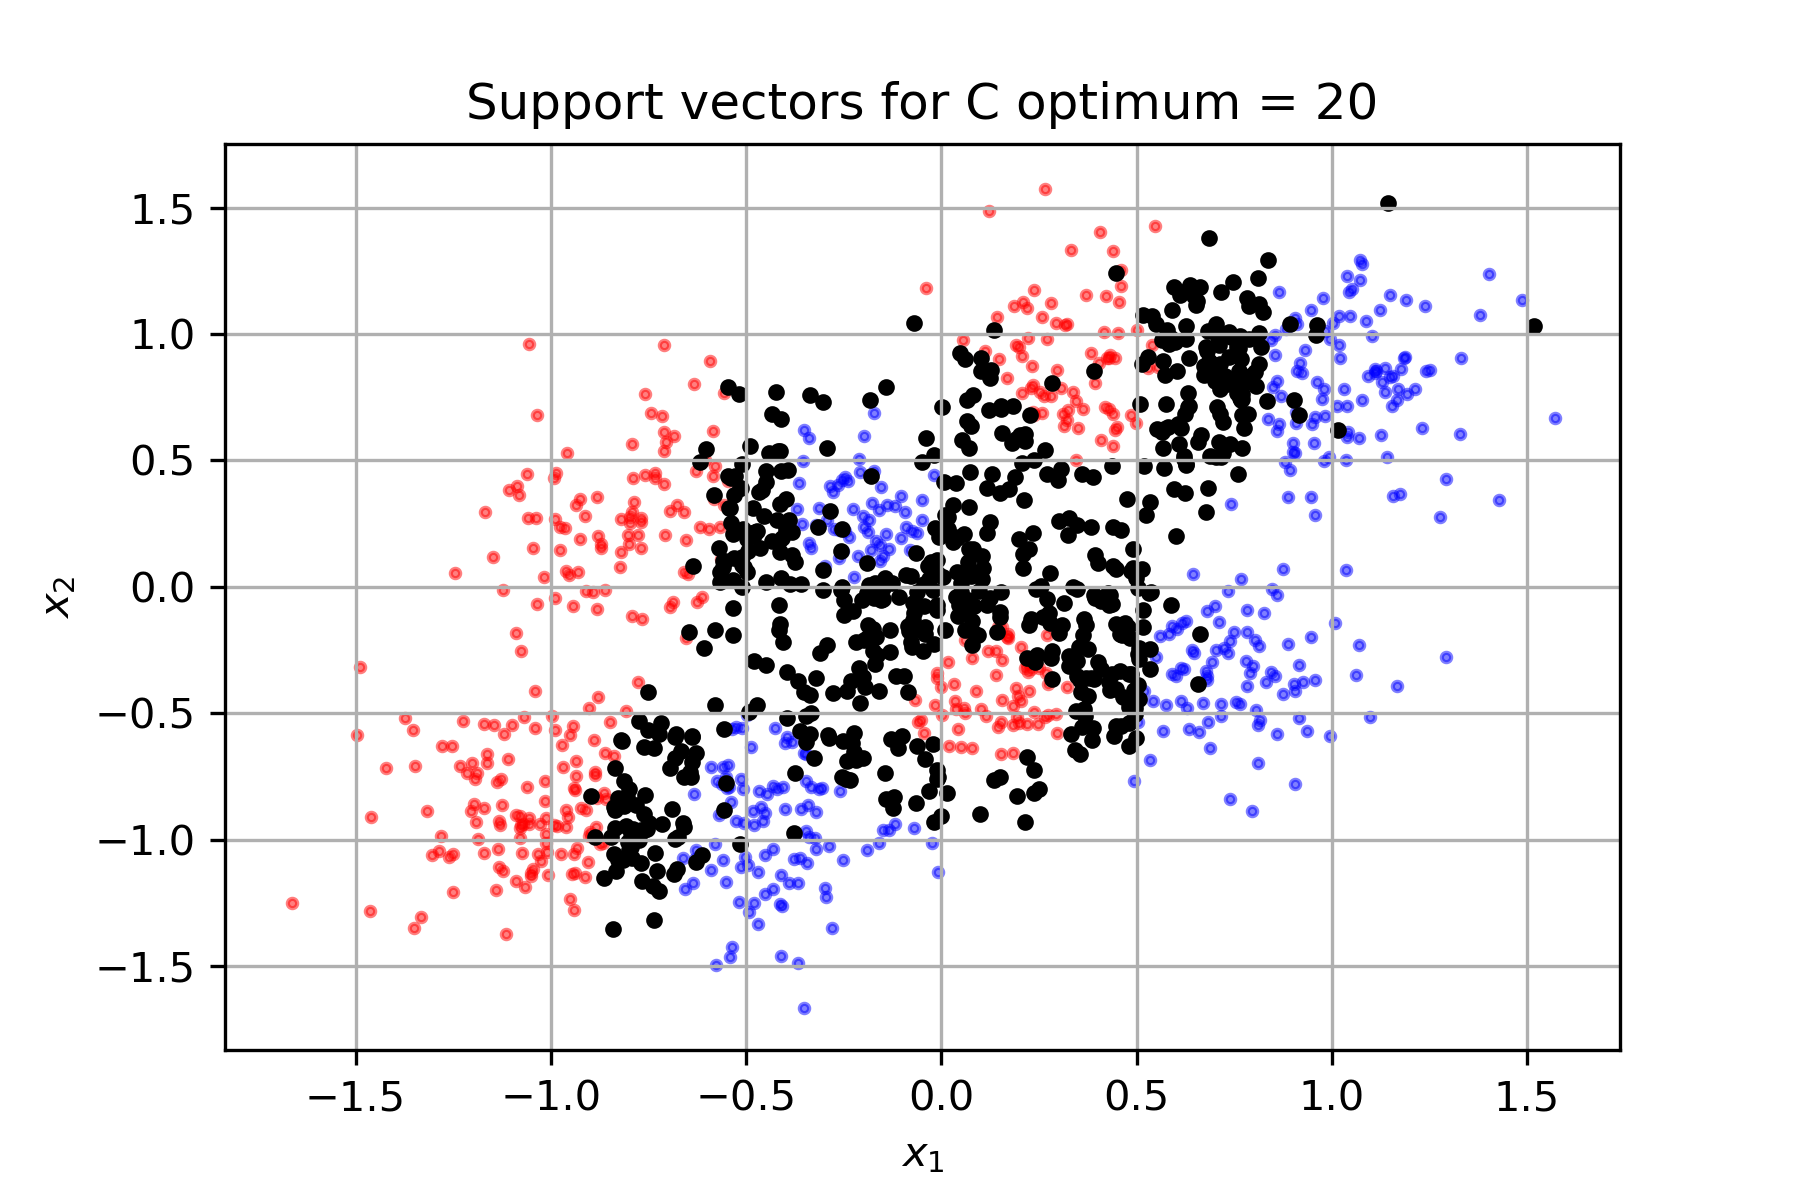
\includegraphics[width=7cm]{support_vectors_C_20}
        \caption{Support vectors for C = 20}
        \label{fig:svm-support_vectors_C_20}
    \end{subfigure}
    %-----------------------------------
    % decision regions (C = 1000)
    \begin{subfigure}{0.45\textwidth}
        \centering
        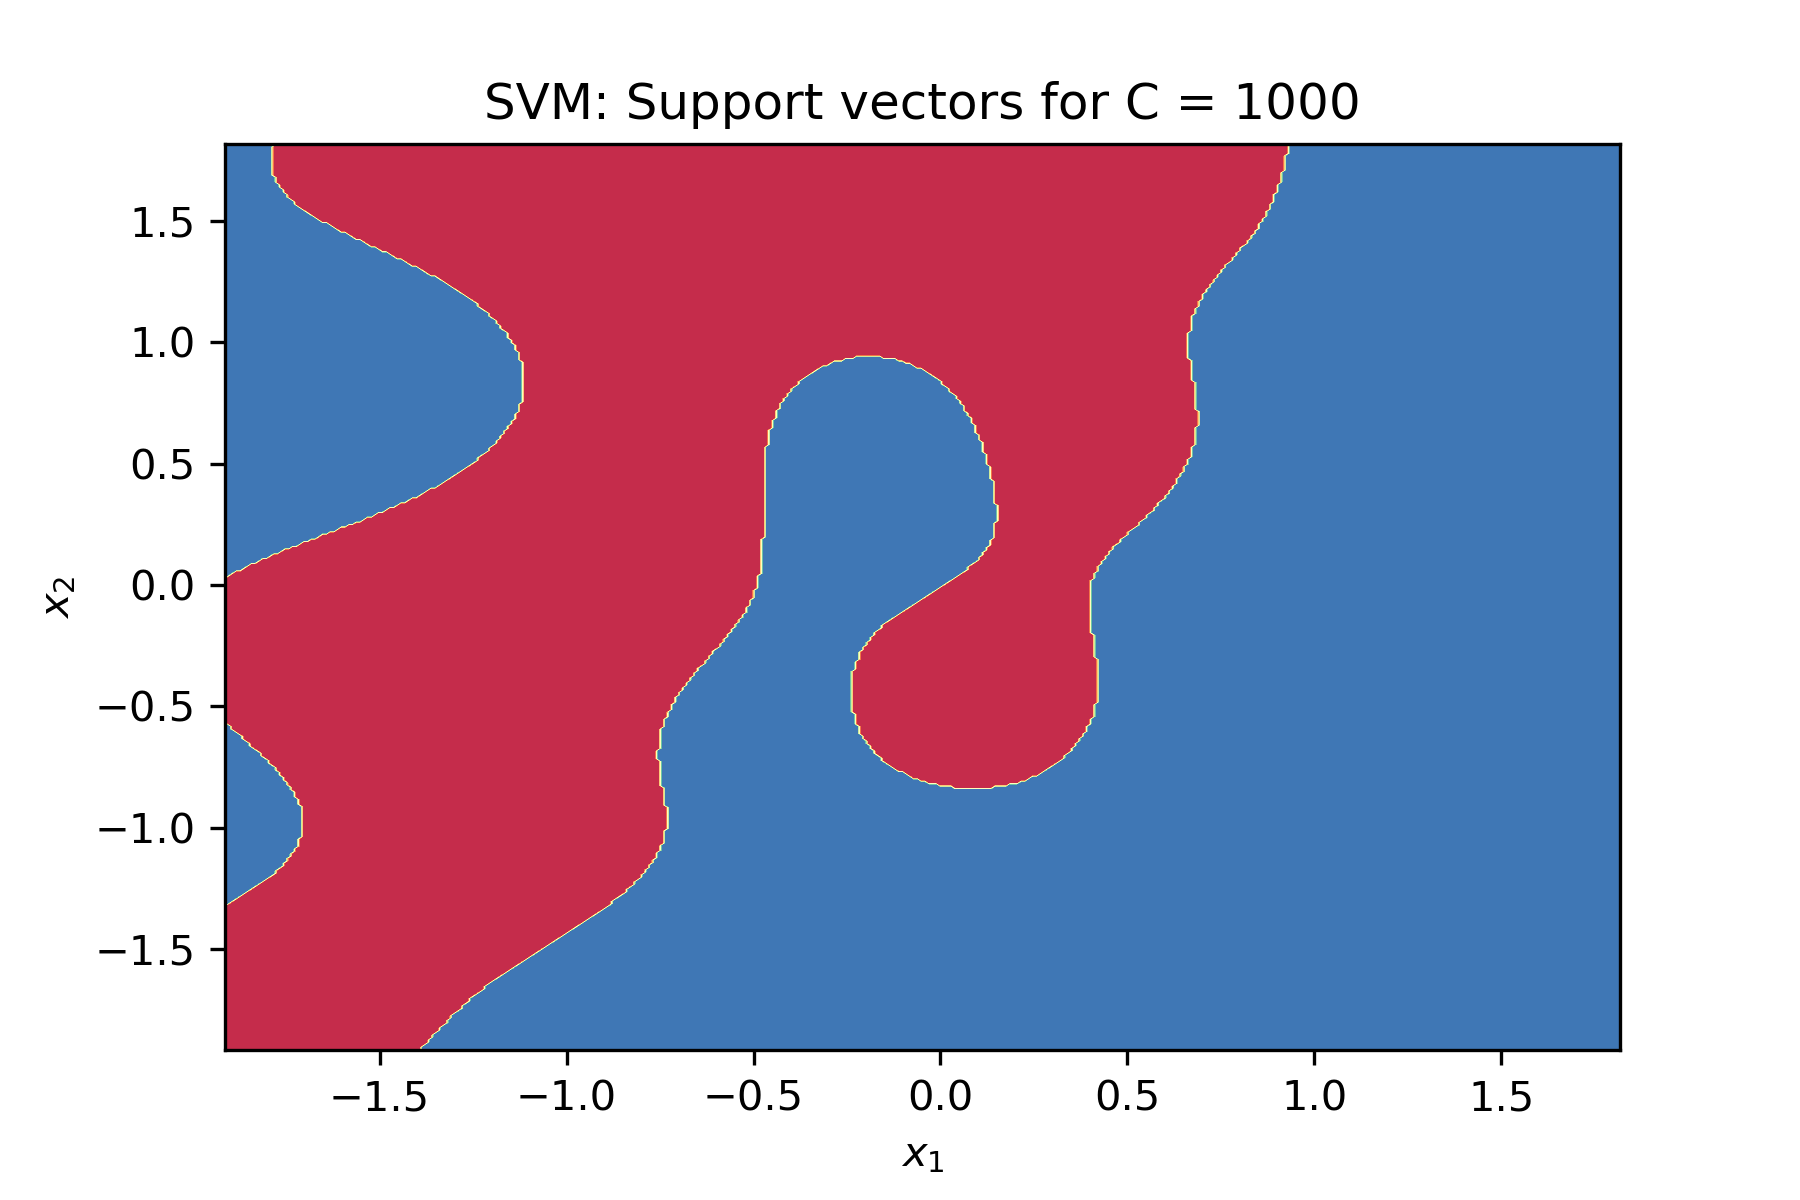
\includegraphics[width=7cm]{decision_region_C_1000}
        \caption{Decision regions for C = 1000}
        \label{fig:svm-decision_region_C_1000}
    \end{subfigure}
    \hfill
    % support vectors (C = 1000)
    \begin{subfigure}{0.45\textwidth}
        \centering
        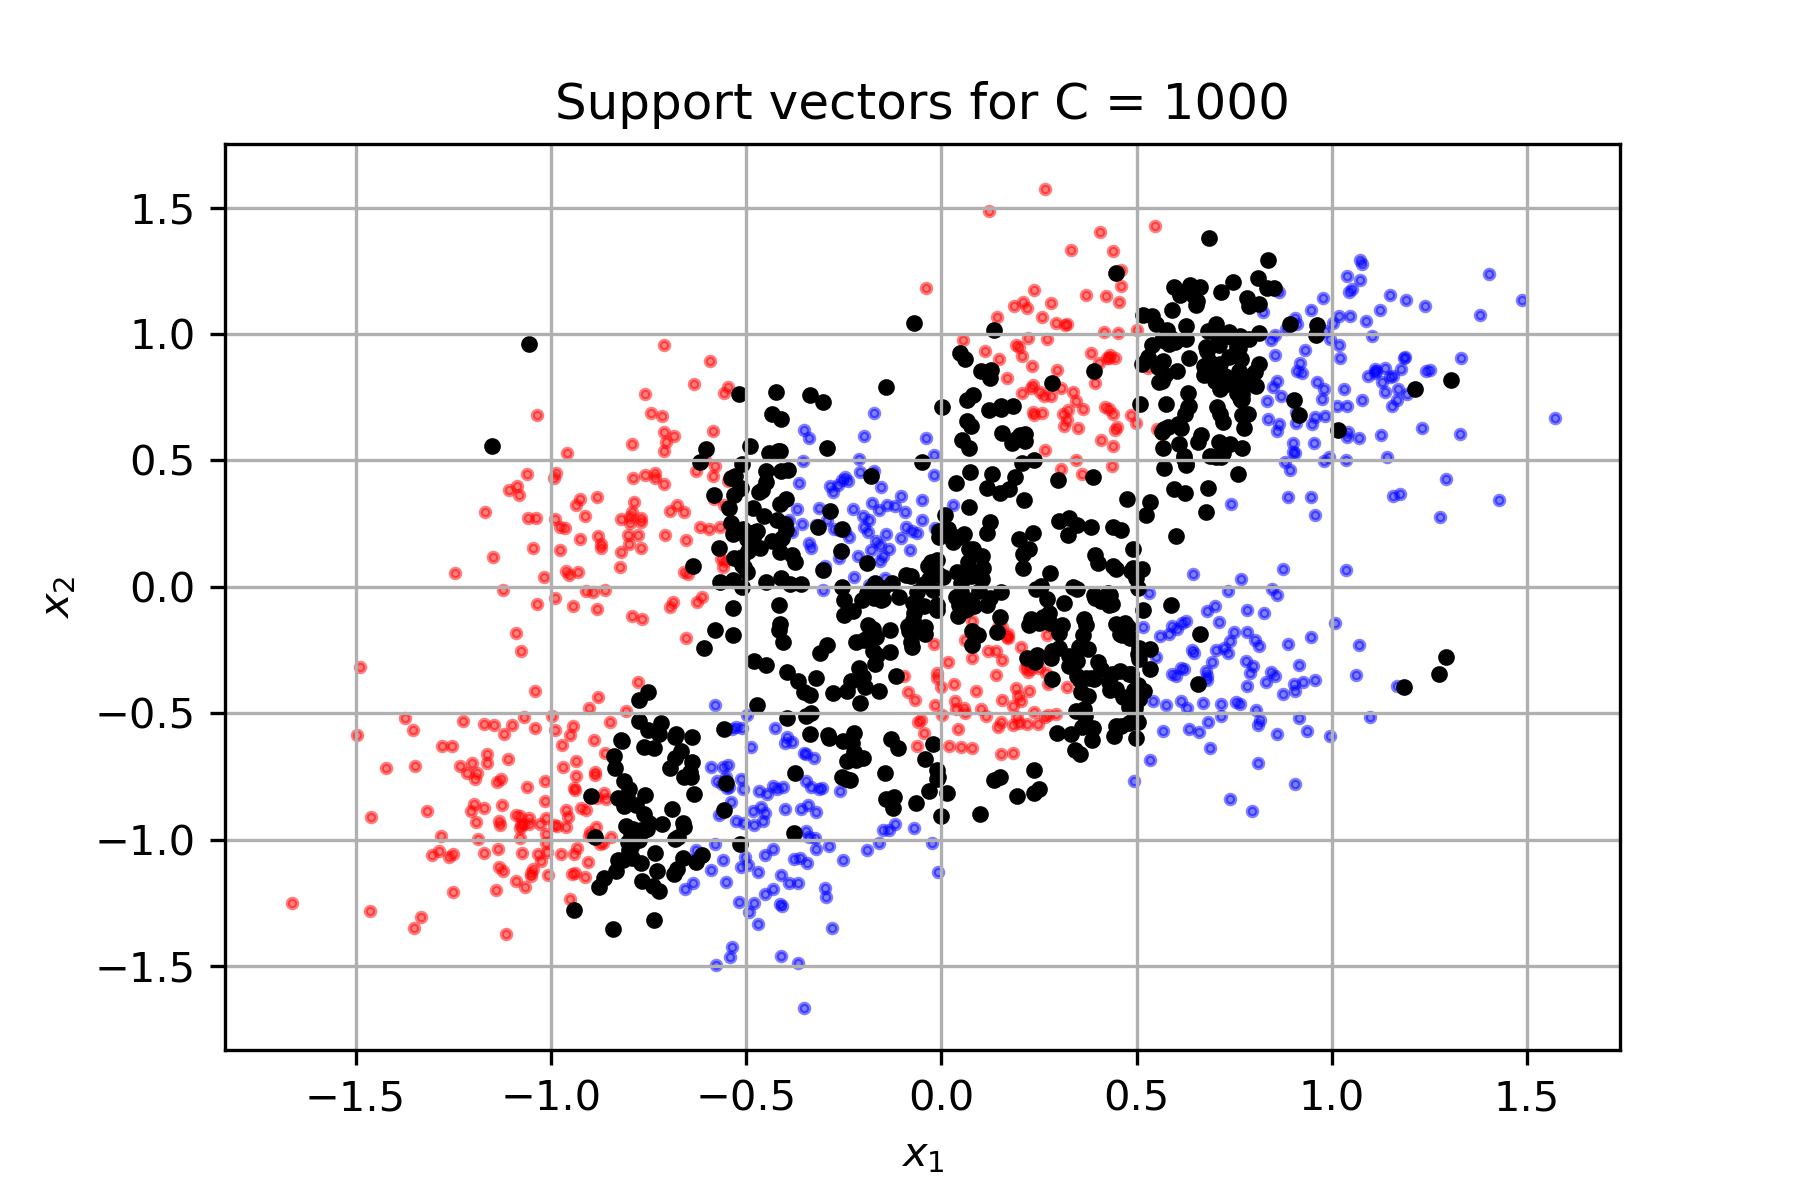
\includegraphics[width=7cm]{support_vectors_C_1000}
        \caption{Support vectors for C = 1000}
        \label{fig:svm-support_vectors_C_1000}
    \end{subfigure}
    %-----------------------------------
    % caption and label
    \caption{Decision regions and respective support vectors for different values of hyperparameter C}
    \label{fig:svm-decision_regions_support_vectos_C}
\end{figure}
%-------------------------------------------------

\paragraph{We can see that for small values of C, we don't give flexibility to the model, suggesting an underfitting. In fact, what we are doing is giving a small weight for the points that invade the border. This produces a rough division in the dataset. We can see that the support vectors are all data near the border.
    The opposite, occurs for example with C = 1000. We are penalizing so much the points that invade the border, that the model will try to fit all data from the training set, leading to an overfitting. This will try to keep only the data very close to the border to be the support vectors.}

\paragraph{We now change the parameter gamma of the Radial Basis Function (RBF) kernel. Values of 0.1, 1 and 10 were used. Figure \ref{fig:svm-decision_regions_support_vectos_gamma} shows the decision regions and the support vectors identified.}

%-------------------------------------------------
%\newpage
% decision regions for different values of hyperparameter gamma
% and the respective support vectors

\begin{figure}[H]
    %-----------------------------------
    \centering
    % decision regions (gamma = 0.1)
    \begin{subfigure}{0.45\textwidth}
        \centering
        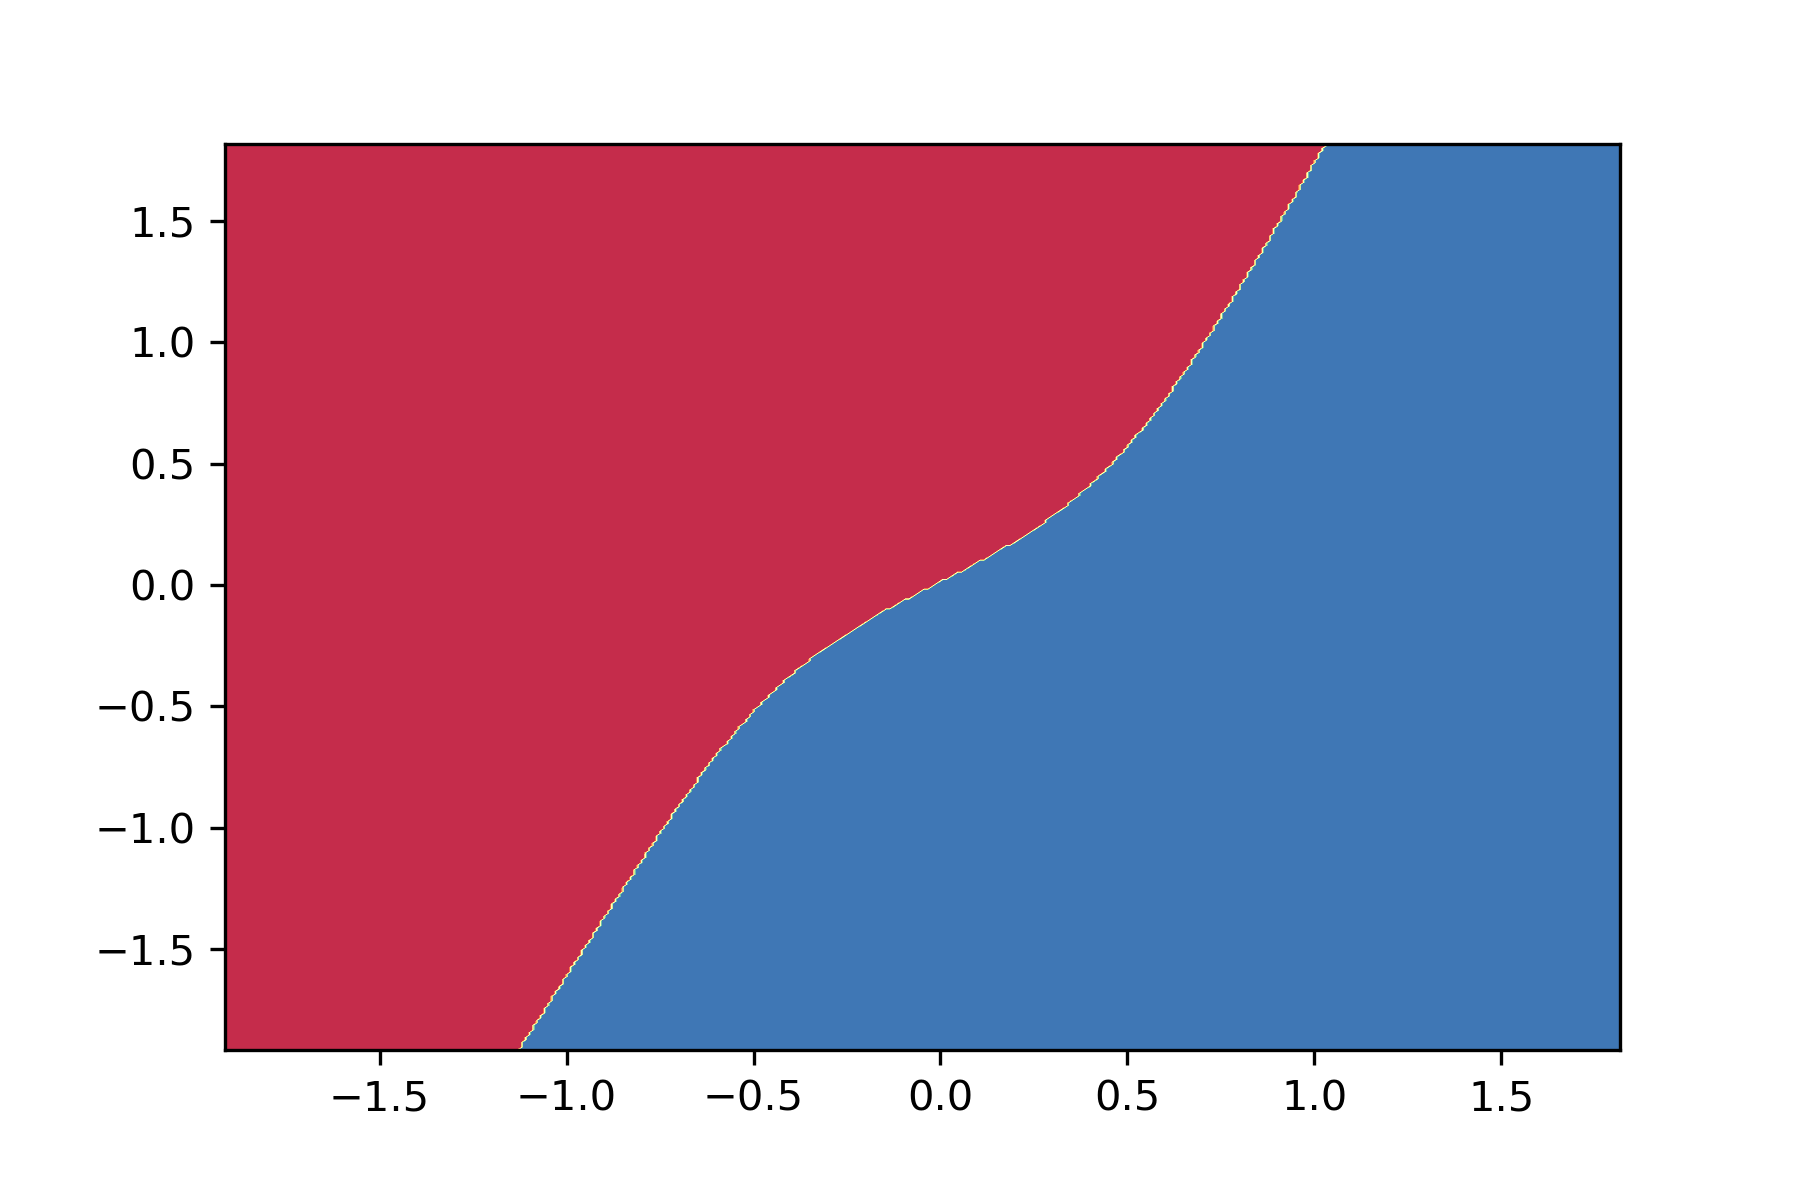
\includegraphics[width=7cm]{decision_region_gamma_0d1}
        \caption{Decision regions for gamma = 0.1}
        \label{fig:svm-decision_region_gamma_0d1}
    \end{subfigure}
    \hfill
    % support vectors (gamma = 0.1)
    \begin{subfigure}{0.45\textwidth}
        \centering
        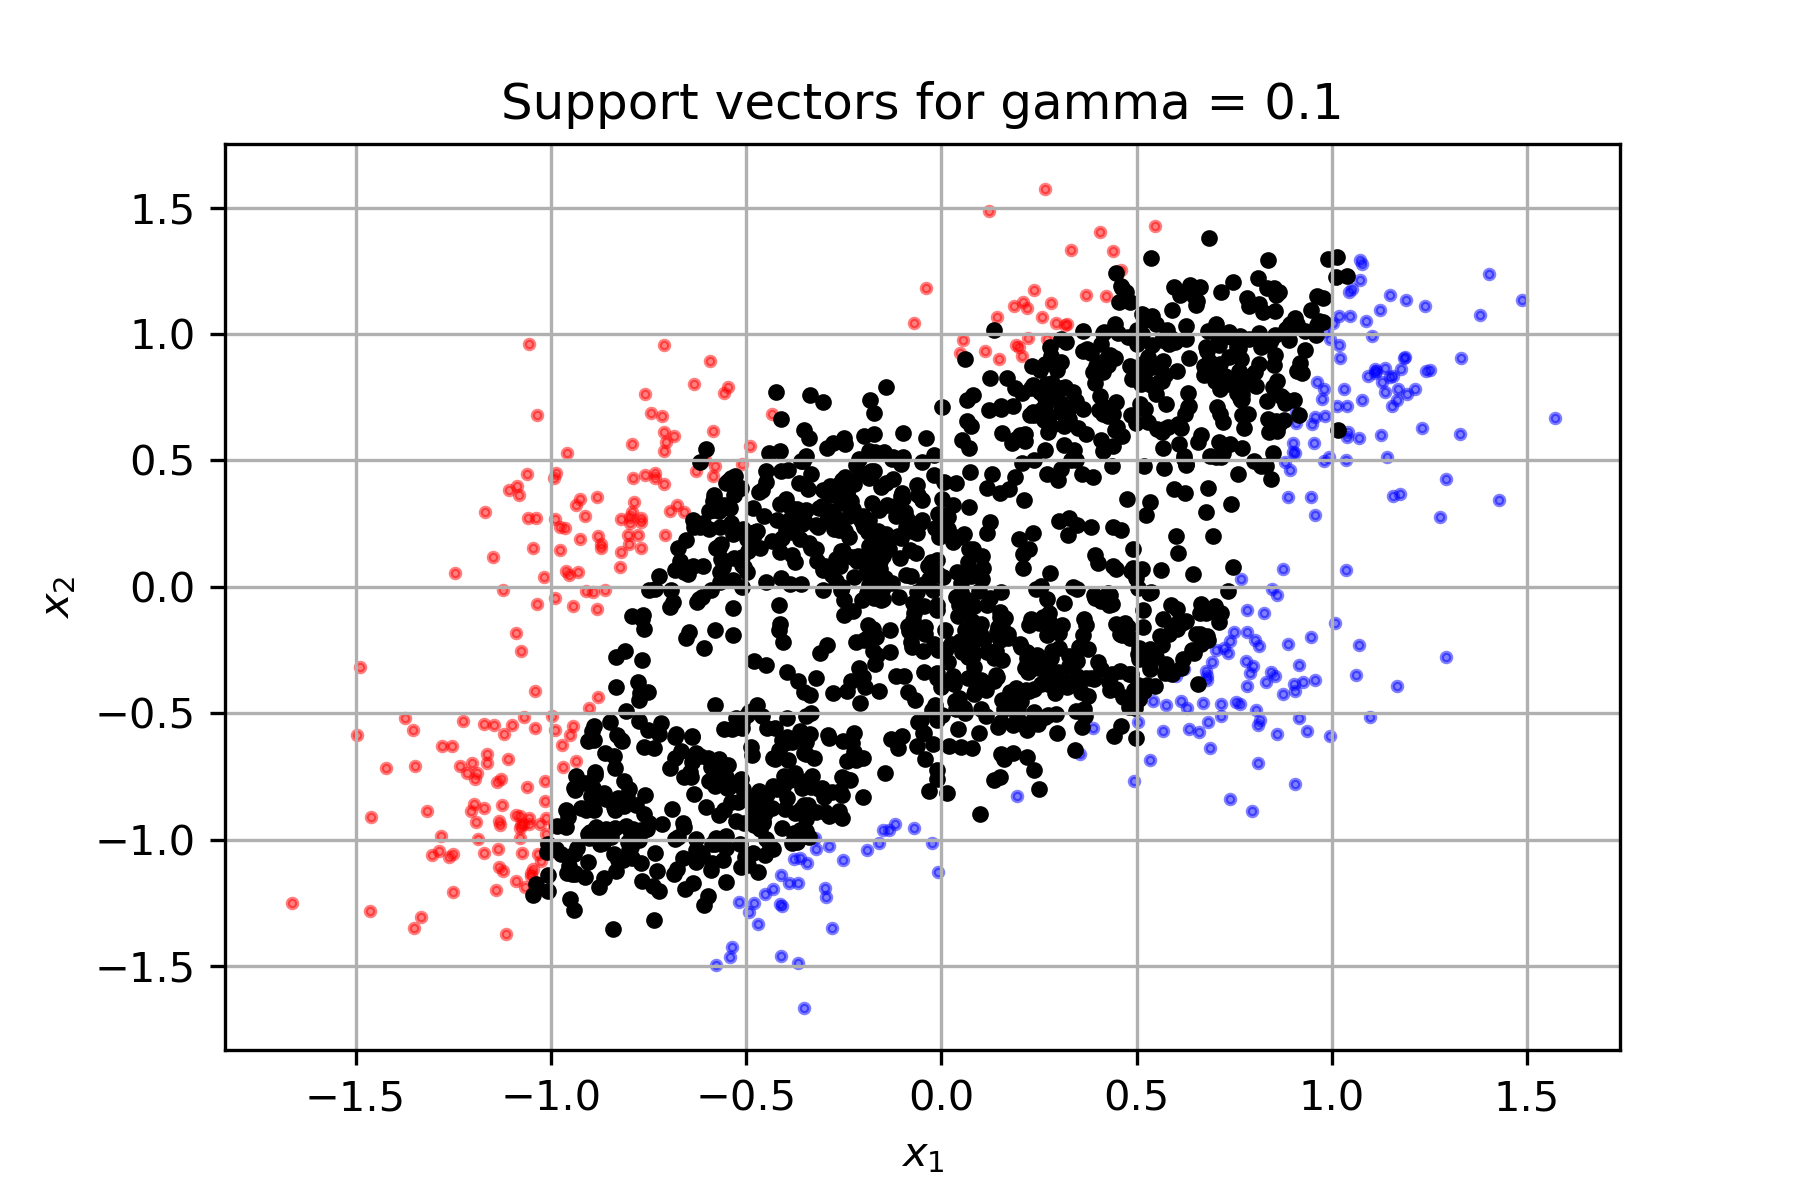
\includegraphics[width=7cm]{support_vectors_gamma_0d1}
        \caption{Support vectors for gamma = 0.1}
        \label{fig:svm-support_vectors_gamma_0d1}
    \end{subfigure}
    %-----------------------------------
    % decision regions (gamma = 1.0)
    \begin{subfigure}{0.45\textwidth}
        \centering
        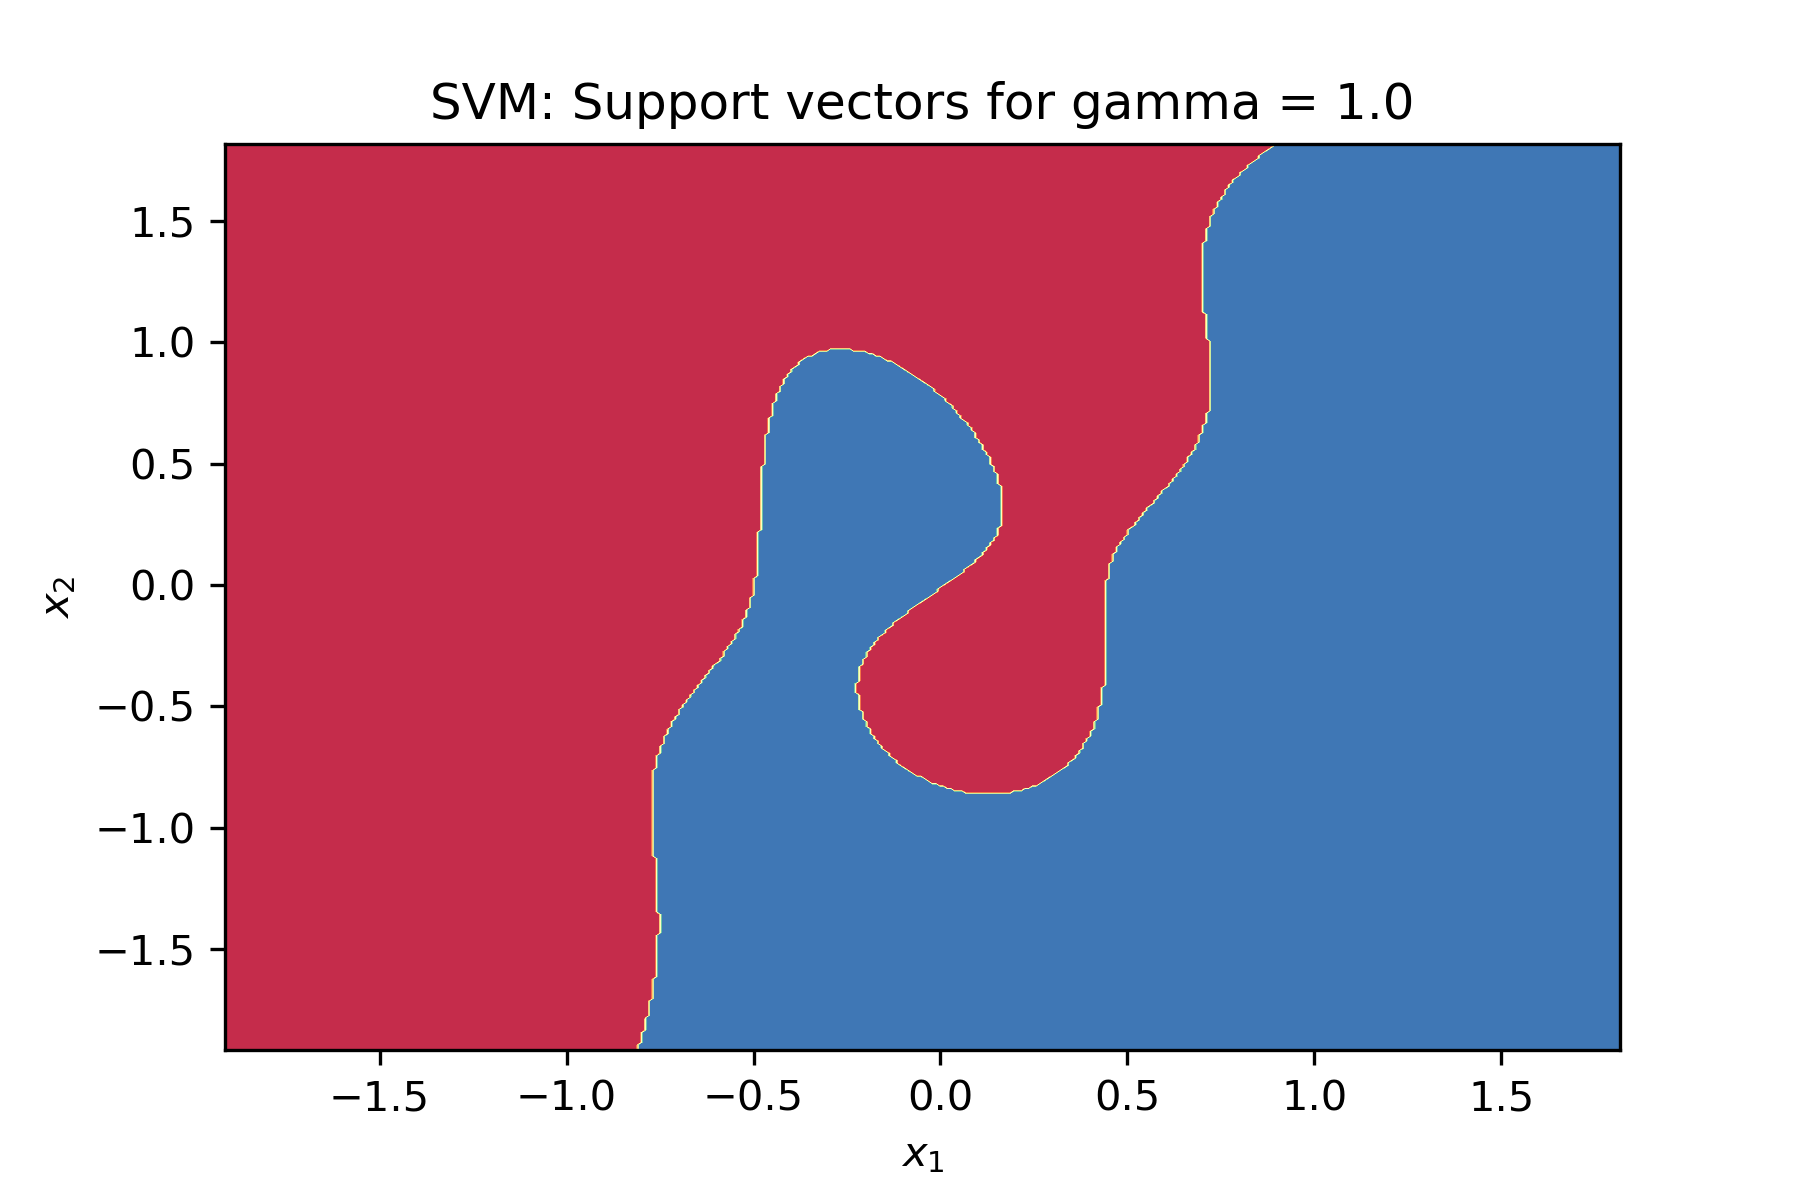
\includegraphics[width=7cm]{decision_region_gamma_1}
        \caption{Decision regions for gamma = 1.0}
        \label{fig:svm-decision_region_gamma_1}
    \end{subfigure}
    \hfill
    % support vectors (gamma = 1.0)
    \begin{subfigure}{0.45\textwidth}
        \centering
        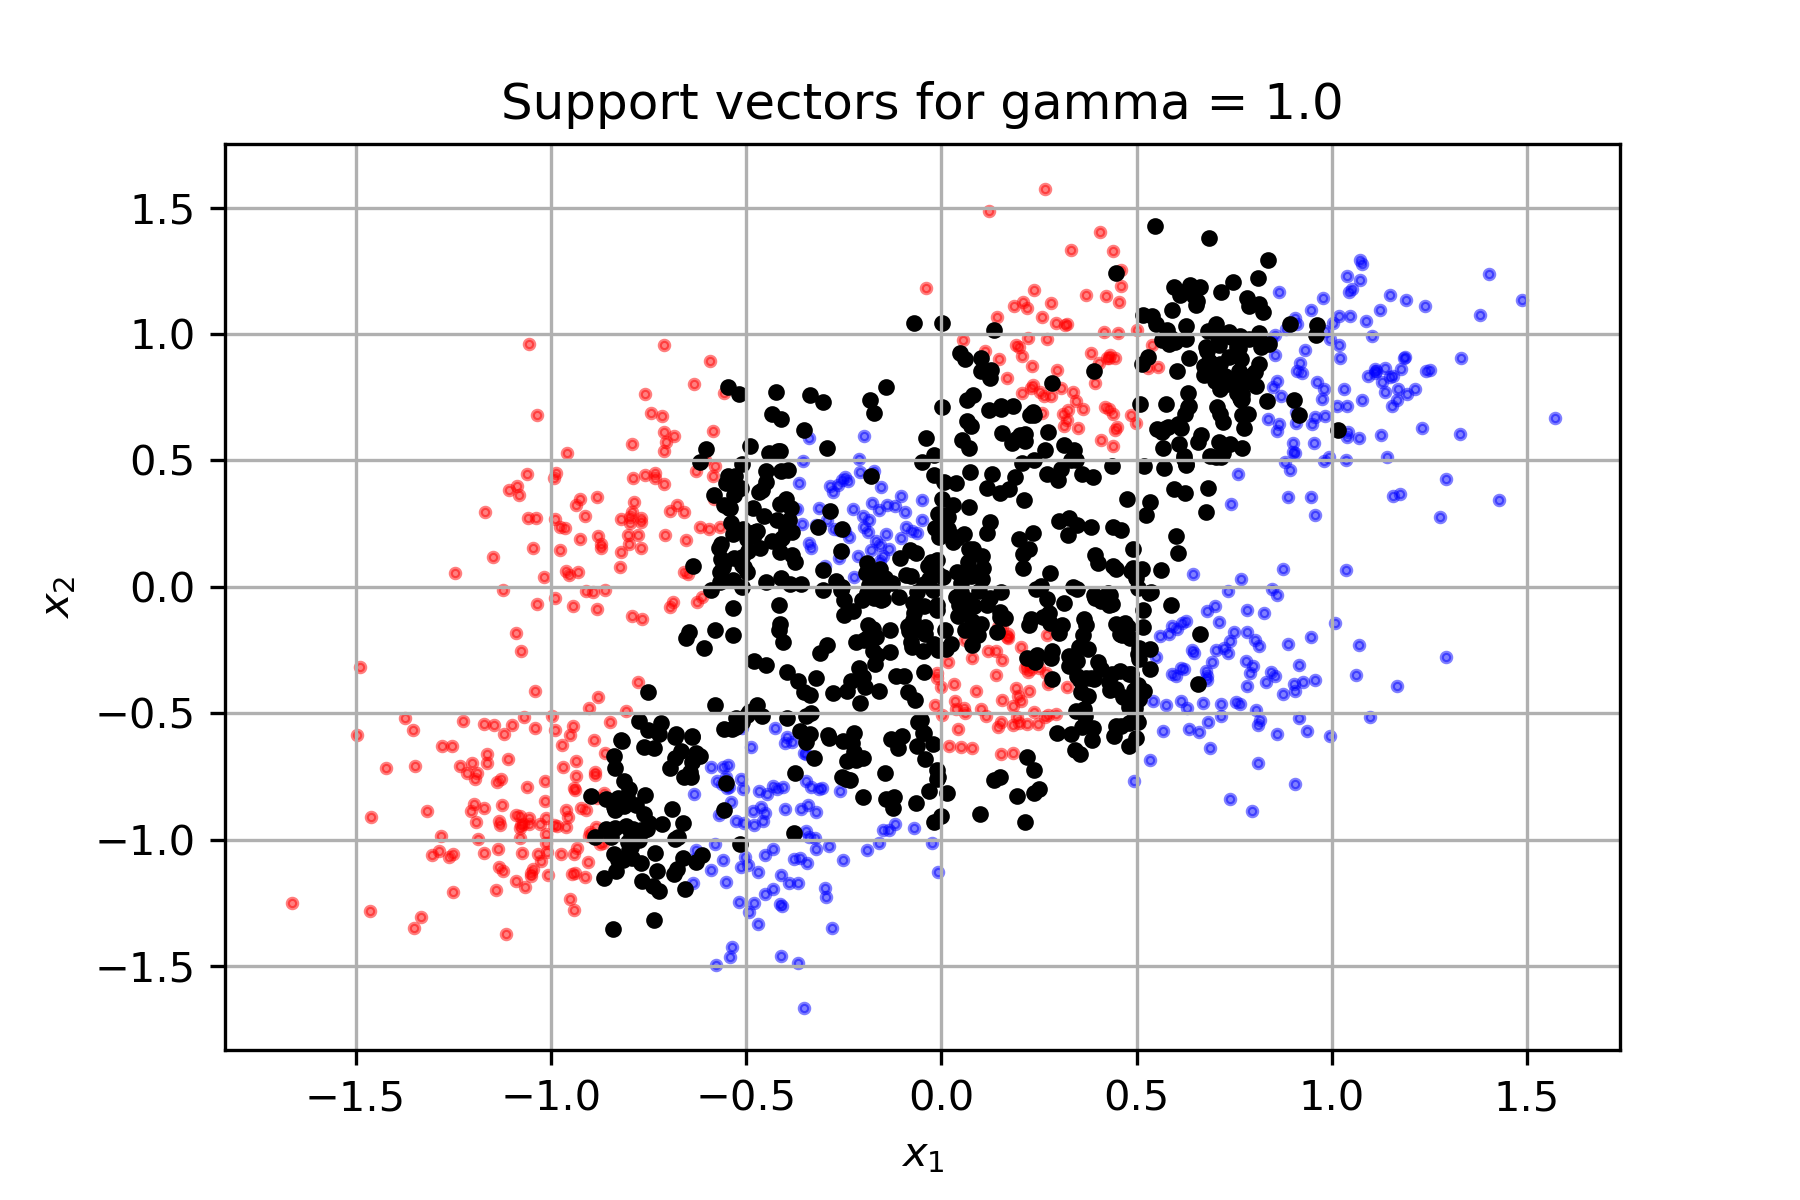
\includegraphics[width=7cm]{support_vectors_gamma_1}
        \caption{Support vectors for gamma = 1.0}
        \label{fig:svm-support_vectors_gamma_1}
    \end{subfigure}
    %-----------------------------------
    %% decision regions (gamma = 20)
    %\begin{subfigure}{0.45\textwidth}
    %    \centering
    %    \includegraphics[width=7cm]{decision_region_gamma_20}
    %    \caption{Decision regions for gamma = 20}
    %    \label{fig:svm-decision_region_gamma_20}
    %\end{subfigure}
    %\hfill
    %% support vectors (gamma = 20)
    %\begin{subfigure}{0.45\textwidth}
    %    \centering
    %    \includegraphics[width=7cm]{support_vectors_gamma_20}
    %    \caption{Support vectors for gamma = 20}
    %    \label{fig:svm-support_vectors_gamma_20}
    %\end{subfigure}
    %-----------------------------------
    % decision regions (gamma = 10)
    \begin{subfigure}{0.45\textwidth}
        \centering
        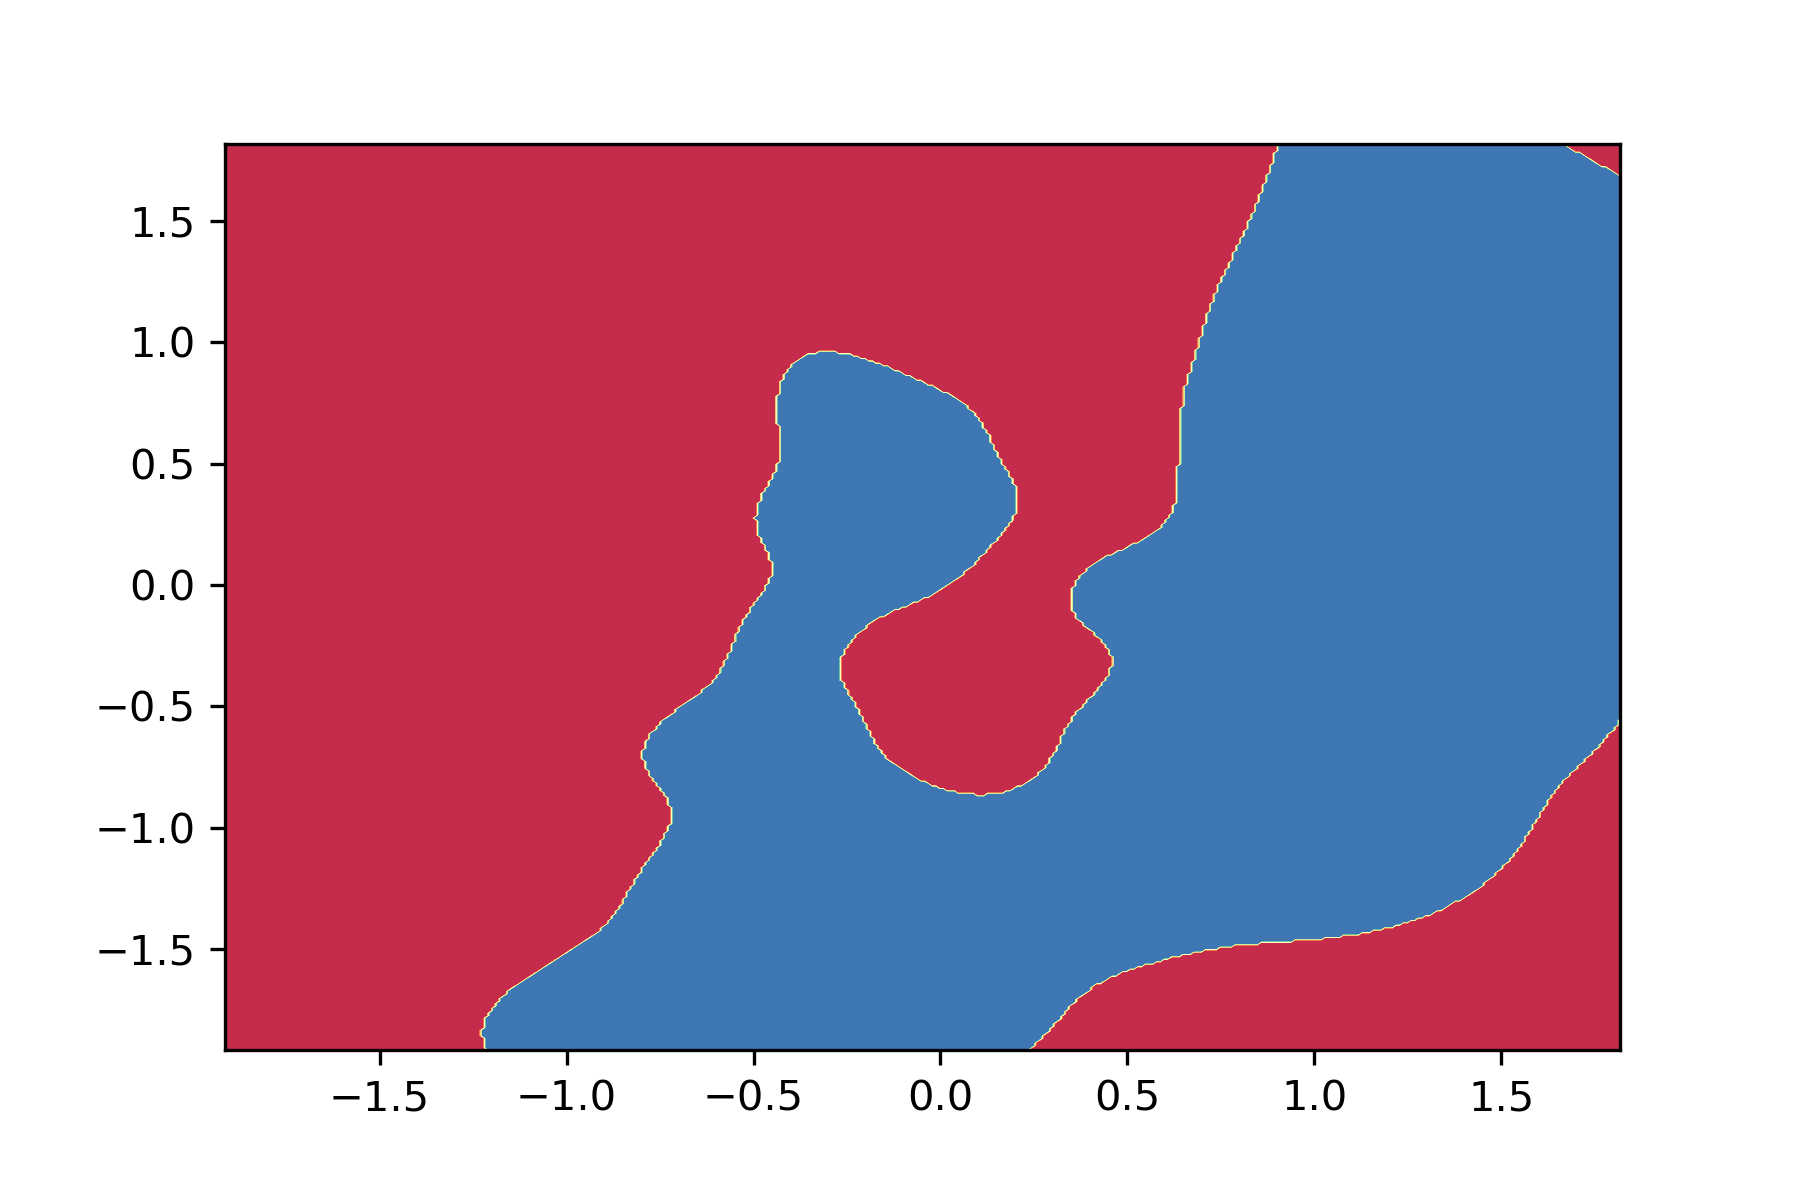
\includegraphics[width=7cm]{decision_region_gamma_10}
        \caption{Decision regions for gamma = 10}
        \label{fig:svm-decision_region_gamma_10}
    \end{subfigure}
    \hfill
    % support vectors (gamma = 10)
    \begin{subfigure}{0.45\textwidth}
        \centering
        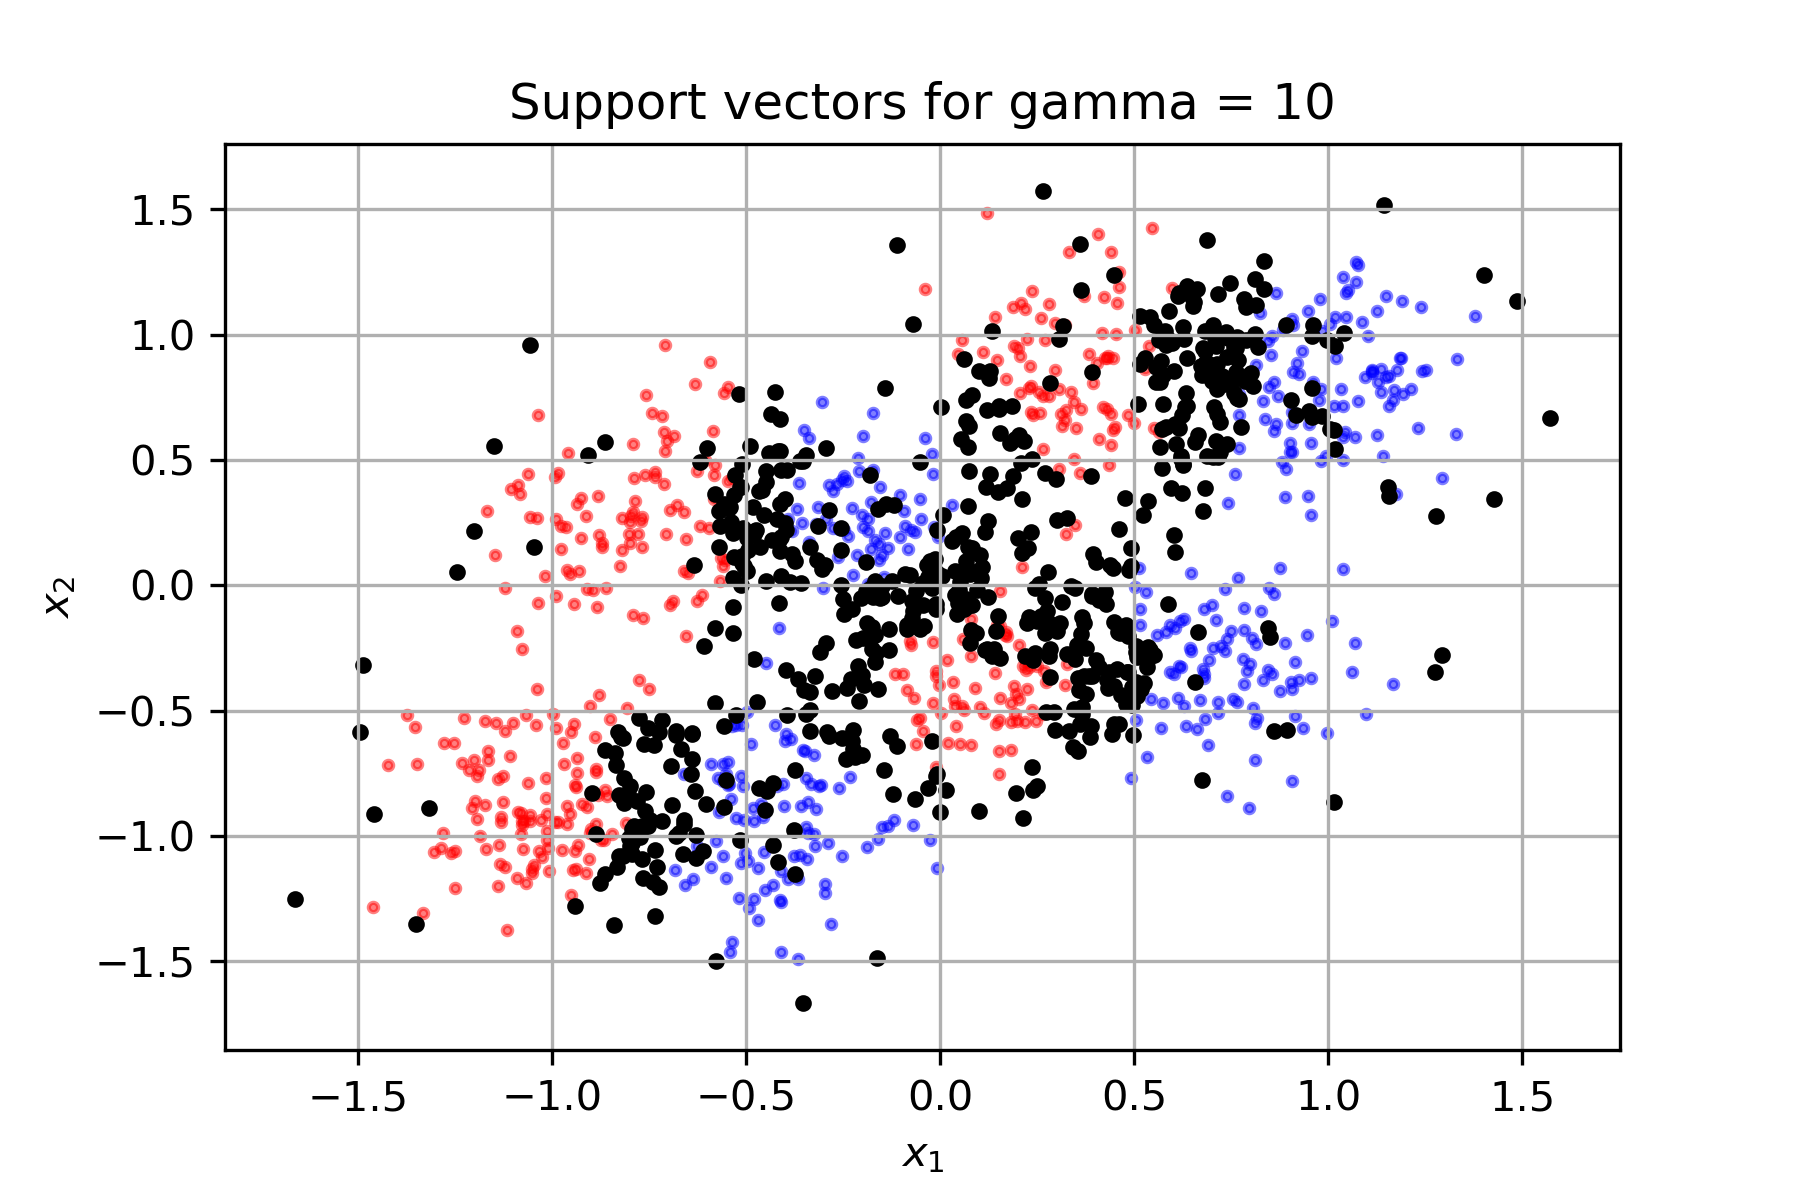
\includegraphics[width=7cm]{support_vectors_gamma_10}
        \caption{Support vectors for gamma = 10}
        \label{fig:svm-support_vectors_gamma_10}
    \end{subfigure}
    %-----------------------------------
    % caption and label
    \caption{Decision regions and respective support vectors for different values of hyperparameter gamma in kernel function}
    \label{fig:svm-decision_regions_support_vectos_gamma}
\end{figure}
%-------------------------------------------------

\paragraph{A similar effect observed with hyperparameter C can be seen here. For small values of gamma, we have a very soft margin, producing a rough classifier and suggesting an underfitting. For gamma equal to 10, the model bent itself to fit almost all data. This leads to a significant generalization loss, indicating an overfitting. Gamma = 1.0 seems to generate a reasonable classifier.}

%=================================================
\end{document}
